% !TEX program = xelatex
\documentclass[UTF8,fontset=fandol,a4paper,11pt]{ctexart}
\usepackage[margin=21mm,top=23mm,bottom=22mm,headheight=16pt]{geometry}
\usepackage{amsmath,amssymb,mathtools,bm}
\usepackage{tikz}
\usetikzlibrary{arrows.meta,calc,angles,quotes,patterns}
\usepackage{xcolor,booktabs,array,longtable,enumitem,fancyhdr,needspace}
\usepackage[unicode,hidelinks]{hyperref}
\definecolor{ink}{HTML}{24343C}
\definecolor{accent}{HTML}{166A70}
\definecolor{muted}{HTML}{65747A}
\definecolor{rulegray}{HTML}{D4DDE0}
\definecolor{warm}{HTML}{966037}
\color{ink}
\setlength{\parindent}{2em}
\setlength{\parskip}{4pt}
\linespread{1.12}
\AtBeginDocument{\setlength{\abovedisplayskip}{6pt plus 2pt minus 1pt}
\setlength{\belowdisplayskip}{6pt plus 2pt minus 1pt}
\setlength{\abovedisplayshortskip}{0pt plus 1pt}
\setlength{\belowdisplayshortskip}{4pt plus 1pt}}
\setlist[enumerate]{label=(\arabic*),leftmargin=2.3em,itemsep=3pt,topsep=4pt}
\setlist[itemize]{leftmargin=2em,itemsep=2pt,topsep=4pt}
\allowdisplaybreaks[1]
\setlength{\emergencystretch}{2em}
\setcounter{secnumdepth}{0}
\providecommand{\tightlist}{\setlength{\itemsep}{0pt}\setlength{\parskip}{0pt}}
\ctexset{section={format=\Large\bfseries\color{accent},beforeskip=10pt,afterskip=9pt},
subsection={format=\normalsize\bfseries\color{accent},beforeskip=10pt,afterskip=4pt},
subsubsection={format=\normalsize\bfseries,beforeskip=8pt,afterskip=3pt}}
\pagestyle{fancy}
\fancyhf{}
\fancyhead[L]{\small\color{muted}物理学难题集萃}
% 页眉仅保留书名；版本名称只在封面显示。
\fancyfoot[L]{\small\color{muted}\chapterlabel}
\fancyfoot[R]{\small\thepage}
\renewcommand{\headrulewidth}{0.4pt}
\renewcommand{\footrulewidth}{0pt}
\newcommand{\dd}{\mathop{}\!\mathrm{d}}
\newcommand{\vect}[1]{\bm{#1}}
\newcommand{\tagline}[1]{\noindent{\small\color{muted}#1}\par}
\newcommand{\result}[1]{\begin{equation*}\boxed{#1}\end{equation*}}
\newcommand{\figcaption}[1]{\par\vspace{2pt}{\small\color{muted}#1}\par}
\newcommand{\teach}[2]{\Needspace{4\baselineskip}\subsection*{讲解要点与追问}#1\par\smallskip\noindent\textbf{追问：}#2\par}
\newcommand{\workarea}{\par\vspace{7mm}\noindent{\small\color{muted}作答区}\par\vspace{4mm}
\noindent\textcolor{rulegray}{\rule{\linewidth}{0.3pt}}\par\vspace{16mm}
\noindent\textcolor{rulegray}{\rule{\linewidth}{0.3pt}}\par\vspace{16mm}
\noindent\textcolor{rulegray}{\rule{\linewidth}{0.3pt}}\par\vspace{16mm}
\noindent\textcolor{rulegray}{\rule{\linewidth}{0.3pt}}}
\tikzset{axis/.style={-{Stealth[length=2mm]},thin,color=muted},
motion/.style={-{Stealth[length=2.3mm]},thick,color=accent},
force/.style={-{Stealth[length=2.3mm]},thick,color=warm},
traj/.style={thick,color=accent},guide/.style={dashed,thin,color=muted},
object/.style={thick,color=ink},every node/.style={font=\small}}\widowpenalty=10000\clubpenalty=10000\displaywidowpenalty=10000

\newcommand{\chapterlabel}{热学第一章\quad 平衡态与理想气体状态方程}
\hypersetup{pdftitle={热学第一章 平衡态与理想气体状态方程·教师版},pdfauthor={},pdfsubject={热学第一章第1--16题}}
\begin{document}
\pdfbookmark[0]{热学第一章 平衡态与理想气体状态方程}{cover}
\thispagestyle{empty}\vspace*{20mm}
\noindent{\Huge\bfseries 物理学难题集萃}\par\vspace{8mm}
\noindent{\LARGE 热学第一章}\par\vspace{5mm}
\noindent{\LARGE 平衡态与理想气体状态方程}\par\vspace{10mm}
\noindent{\Large\color{accent}教师版}\par\vspace{8mm}
\noindent\textcolor{accent}{\rule{\linewidth}{1pt}}\par\vspace{8mm}
\noindent 第1--16题\par\vspace{5mm}
\noindent 详细解答、备课分析、课堂追问与变式训练。\par\vfill\clearpage
\pdfbookmark[1]{题目目录}{contents}\section*{题目目录}
\begin{longtable}{@{}>{\color{accent}\bfseries}r p{120mm}@{}}
\toprule 题号 & 题目\\\midrule
1 & 道尔顿定压温标与摄氏温度换算 \\
2 & 热电偶非线性电动势与自定温标 \\
3 & 多只贮气罐给真空室逐次充气 \\
4 & U形管注入水银后的封闭气体压强 \\
5 & 玻璃管倒置插入水银槽的双气柱变化 \\
6 & 升温推动水银柱外溢的分阶段判断 \\
7 & 试管倒置时两端封气长度的比较 \\
8 & 湖底水箱充气上浮所需空气量 \\
9 & 热气球刚好升空的内部温度 \\
10 & 浮沉子受压下沉的速度关系 \\
11 & 由行星大气压强曲线求探测器速度 \\
12 & 用体积百分比求标准状态空气密度 \\
13 & 干湿空气浮力差导致的称量差异 \\
14 & 干空气与湿空气隔板平衡及混合压强 \\
15 & 潮湿空气压缩凝结与降温后的压强 \\
16 & 可分解双原子气体升温后的水银柱移动 \\\bottomrule\end{longtable}

\clearpage

\pdfbookmark[2]{第 1 题 道尔顿定压温标与摄氏温度换算}{q1}

\section*{第 1 题\quad 道尔顿定压温标与摄氏温度换算}

道尔顿定压温标以一定量理想气体的体积为测温属性：在压强恒定时，体积的相对微小增量正比于温度读数$\tau$的增量，即$\dd V/V=A\dd\tau$，$A$为常量。冰点规定为$\tau=0^\circ$，汽点规定为$\tau=100^\circ$。试用摄氏温度$t$表示$\tau$。

\begin{center}\begin{minipage}{0.96\linewidth}\centering
\begin{tikzpicture}[x=1cm,y=1cm]\fill[accent!8] (0, 0) rectangle (2,2.2);
\node[align=center,font=\footnotesize] at (1.0,1.1) {气体 $V$\\$p$恒定};
\fill[warm!30] (0, 2.2) rectangle (2,2.3200000000000003);
\node[align=center,font=\footnotesize] at (1.0,2.2600000000000002) {};
\draw[object] (0,0)--(0,2.3200000000000003);\draw[object] (2,0)--(2,2.3200000000000003);
\draw[object] (0,0)--(2,0);
\node[align=center] at (1.0,-.55) {气体温度计};

\draw[motion] (1,2.5)--(1,2.9);
\node at (4.6,2.3) {冰点：$V_0,\ \tau=0$};
\node at (4.6,1.2) {汽点：$V_{100},\ \tau=100$};
\node at (4.6,.2) {$\dd V/V=A\dd\tau$};
\end{tikzpicture}\figcaption{图 热1.1　定压条件下用体积读数建立温标。}\end{minipage}\end{center}

\Needspace{5\baselineskip}

\pdfbookmark[3]{题型定位}{q1-h0}

\subsection*{题型定位}

温标定义与两点定标题。先把相对体积的微分规定积分成读数函数，再用等压理想气体方程换成摄氏温度。题目的难点在于辨认$\dd V/V$，并区分温标的定义和气体的状态规律。

\Needspace{5\baselineskip}

\pdfbookmark[3]{知识点}{q1-h1}

\subsection*{知识点}

温标由测温物质、测温属性、固定点和读数变化规律共同确定。本题取一定量理想气体及其恒压体积，冰点、汽点固定两个读数，$\dd V/V=A\dd\tau$规定中间刻度。
理想气体等压时$V/V_0=T/T_0$，其中$T$为绝对温度；摄氏数值$t$通过$T=T_0+t$进入换算。
积分只含体积比，因此 $A$ 的量纲是道尔顿度的倒数。
指数关系$V/V_0=e^{A\tau}$与对数反解等价；导数判断单调性和凹凸性，泰勒展开只在$|t|\ll T_0$时给冰点附近的近似线性关系。
双点定标确定比例常数，却不改变已经规定的函数形式。

\Needspace{5\baselineskip}

\pdfbookmark[3]{物理图像}{q1-h2}

\subsection*{物理图像}

图热1.1中的活塞使气体在定压下改变体积，$V$正比于$T$。温度计每增加相同的道尔顿读数，体积乘以相同倍数；解图热1.1B的三柱分别是$V_0,qV_0,q^2V_0$。因$q>1$，后一段50度所需的体积增量较大。
解图热1.1A以摄氏数值作横轴，道尔顿数值作纵轴。曲线经过两固定点，斜率随横坐标增大而下降；两固定点之间的读数差由这条曲线与$\tau=t$直线的纵向间隔给出。解图热1.1B给出相邻读数的体积比，解图热1.1A把这一关系换算成温度读数。

\Needspace{5\baselineskip}

\pdfbookmark[3]{解题入口}{q1-h3}

\subsection*{解题入口}

先将未知常数保留为$A$，以冰点状态作积分下限，得到$\ln(V/V_0)=A\tau$。此时先不代摄氏温度，避免将线性刻度混入温标定义。
再用同一份气体的$V/V_0=T/T_0$消去体积，最后代汽点确定$A$。冰点固定积分常数，汽点固定读数的比例；两个条件在推导中各有作用。
学生若直接写$\tau=t$，可请其求$\dd\tau/\dd t$：定义和状态方程联立给$1/[A(T_0+t)]$，已显示斜率不恒定。

\Needspace{5\baselineskip}

\pdfbookmark[3]{标准解法}{q1-h4}

\subsection*{标准解法}

\textbf{从温标定义积分。}图热1.1中的气体始终保持定压、定量。温标按体积的\emph{相对}增量分刻度；比例常量 $A$ 由后面的汽点条件确定。以冰点体积$V_0$为积分下限：
\[\int_{V_0}^{V}\frac{\dd V'}{V'}=A\int_0^\tau\dd\tau',\qquad
\ln\frac{V}{V_0}=A\tau.\]
若把一个总温标增量分成许多相同小格$\Delta\tau$，每一格令体积乘约$1+A\Delta\tau$。经过$N$格后，
\[V/V_0\simeq(1+A\Delta\tau)^N
\longrightarrow e^{A\tau},\qquad N\Delta\tau=\tau.\]
解图热1.1B中相等的读数间隔对应相同体积比，积分得到对数换算。该式只涉及温标的定义，实际气体的绝对温度关系随后另由状态方程代入。

对同一份理想气体，$pV=nRT$给出
\[\frac{V}{V_0}=\frac{T}{T_0}=1+\frac{t}{273.15},\qquad T_0=273.15\,\mathrm K.\]
其中$t$按摄氏度的数值代入。于是
\[\tau=\frac1A\ln\left(1+\frac{t}{273.15}\right).\]
\textbf{用汽点定标。}把$t=100$、$\tau=100$代入，得到
\[A=\frac1{100}\ln\frac{373.15}{273.15}
=0.00311959\ (\text{道尔顿度})^{-1}.\]
\result{\tau=\frac{100\ln(1+t/273.15)}{\ln(373.15/273.15)}
\approx320.6\ln(1+t/273.15).}
\Needspace{26\baselineskip}
\begin{center}\begin{minipage}{0.96\linewidth}\centering
\begin{tikzpicture}[x=1cm,y=1cm]
\draw[axis] (0,0)--(6,0) node[right] {$t/{}^\circ\mathrm C$};
\draw[axis] (0,0)--(0,4.6) node[above] {$\tau/{}^\circ$};
\draw[traj,domain=0:5.3,samples=90] plot (\x,{2*ln(1+50*\x/273.15)/ln(373.15/273.15)});
\draw[guide] (0,0)--(4.35,4.35) node[above right] {$\tau=t$};
\foreach \x/\y/\lab in {.9221679/1/{46.1},2/2/{100},4/3.522198004/{200}}{
 \draw[guide] (\x,0) node[below] {$\lab$}--(\x,\y)--(0,\y);
}
\node[left] at (0,1) {50};\node[left] at (0,2) {100};
\fill[accent] (2,2) circle(1.5pt);\node[above left] at (2,2) {汽点};
\node[below left] at (0,0) {冰点};
\end{tikzpicture}\figcaption{解图 热1.1A　对数曲线与直线交于冰点、汽点，纵向距离给出两温标的读数差。}\end{minipage}\end{center}
解图热1.1A经过冰点和汽点，但曲线向下凹。确实，若记$C=100/\ln(373.15/273.15)>0$，则
\[\frac{\dd\tau}{\dd t}=\frac{C}{273.15+t}>0,\qquad
\frac{\dd^2\tau}{\dd t^2}=-\frac{C}{(273.15+t)^2}<0.\]
因而在理想气体模型的$t>-273.15$范围内可唯一反解：
\[t=273.15\bigl(e^{A\tau}-1\bigr).\]
当$|t|\ll273.15$时，$\tau\approx(C/273.15)t\approx1.174t$。两温标在固定点处读数相同，在点间则各自按测温属性的变化规律取值，因此读数差随温度而改变。
\subsubsection*{定标点之间的具体读数与体积}
在两个定标点之间，道尔顿温标以体积的相对变化分刻度。由于同一份气体的等压体积正比于绝对温度，体积比也就是两状态的开尔文温度比。

把定义写成有限区间的积分，有
\[
\ln\frac{V_2}{V_1}=A(\tau_2-\tau_1),\qquad
\frac{V_2}{V_1}=e^{A(\tau_2-\tau_1)}.
\]
所以相等的道尔顿读数间隔给出相同的体积比。解图热1.1B取三个读数0、50、100。

令$q=\sqrt{373.15/273.15}$，三次体积依次为$V_0,qV_0,q^2V_0$；
相邻体积差为$(q-1)V_0$与$q(q-1)V_0$，后一段更大。
\begin{center}\begin{minipage}{0.96\linewidth}\centering
\begin{tikzpicture}[x=1cm,y=1cm]
\foreach \x/\h/\lab/\temp in {0/1.6/{V_0}/0,2.9/1.870083951/{qV_0}/50,5.8/2.18576/{q^2V_0}/100}{
 \fill[accent!8] (\x,0) rectangle ++(1.4,\h);
 \draw[object] (\x,\h)--(\x,0)--++(1.4,0)--++(0,\h);
 \draw[object] (\x,\h)--++(1.4,0);
 \node[above] at (\x+.7,\h) {$\lab$};
 \node[below] at (\x+.7,0) {$\tau=\temp$};
}
\draw[motion] (1.5,1.15)--(2.7,1.15) node[midway,above] {$\times q$};
\draw[motion] (4.4,1.15)--(5.6,1.15) node[midway,above] {$\times q$};
\node at (3.6,-.85) {$p,n$相同，截面积相同；柱高正比于$V$};
\end{tikzpicture}
\figcaption{解图 热1.1B　两段50度的读数间隔对应相同体积比，后一段体积增量较大。}
\end{minipage}\end{center}
图中间那一柱的绝对温度是几何平均值：
\[
T_{50}=\sqrt{273.15\times373.15}\,\mathrm K,\qquad
t_{50}=46.1084^\circ\mathrm C.
\]
反过来，摄氏中点$t=50^\circ\mathrm C$给$\tau=53.8838^\circ$。
解图热1.1A 中，从纵轴的 $\tau=50$ 水平移到曲线，再向下读横坐标。已知摄氏温度时，则从横轴竖直到曲线，再移到纵轴读取 $\tau$。

对任意两个状态，定义还给出
\[
\Delta\tau=\frac1A\ln\frac{T_2}{T_1}
=\frac1A\ln\left(1+\frac{\Delta t}{273.15+t_1}\right).
\]
同样的摄氏温差在较高起始温度处给出较小的道尔顿读数差。
当$|\Delta t|\ll273.15+t_1$时，局部斜率为$1/[A(273.15+t_1)]$；
在冰点约为1.17355，在汽点约为0.859050。
解图热1.1A中随温度升高而减小的斜率正对应这一变化。
两端定标还要求$\tau(0)=0$、$\tau(100)=100$，
且$t\to-273.15^+$时$\tau\to-\infty$；这些是所给理想气体温标的数学极限。
这里的极限沿理想气体方程取；使用实际气体定标时，体积比由该气体的等压状态关系给出。


\Needspace{5\baselineskip}

\pdfbookmark[3]{关键洞察}{q1-h5}

\subsection*{关键洞察}

对数由相对体积增量的定义产生。保持气体的等压状态规律不变，只改读数的定义，就能得到另一种非线性温标。
读数中点$\tau=50$对应绝对温度的几何平均值，而摄氏中点$t=50$对应绝对温度的算术平均值；前者为46.1084℃，后者读作53.8838度。几何平均小于算术平均，因此读数中点在摄氏中点的左侧。
有限温差换算还依赖起始温度，同样的摄氏温差在高温处给出更小的道尔顿读数差。

\Needspace{5\baselineskip}

\pdfbookmark[3]{易错点}{q1-h6}

\subsection*{易错点}

若把$\dd V/V$换成$\dd V$，积分会误得线性温标；应在板书中保留分母$V$并注明其为变化量。
只代冰点会使$A$仍未确定，过早以273代273.15又会改变最后的数值系数。气体状态方程里的温度是$T$，对数的自变量应为$T/T_0$；直接写$\ln t$既有量纲问题，也无法处理冰点。
局部近似的自变量是$t/T_0$，称作“冰点附近”比笼统称作“低温”准确。摄氏数值$t$与温差$\Delta t$也应分开：有限温差的读数差随起始温度 $t_1$ 改变。
在 $t>-273.15$ 的理想气体模型内，读数函数严格递增，因而每个读数对应一个摄氏温度。

\Needspace{5\baselineskip}

\pdfbookmark[3]{课堂讲解建议}{q1-h7}

\subsection*{课堂讲解建议}

先列出温标的测温属性和微分规定，要求学生分别写$\dd V=B\dd\tau$与$\dd V/V=A\dd\tau$的积分结果。前者给体积差，后者给体积比，再联系同一份气体的$V\propto T$。
在解图热1.1B上遮住中柱体积，问相邻两段都是50度时，中柱应取体积的算术平均还是几何平均。由$V_{50}^2=V_0V_{100}$求出实际温度46.1084℃，随后在解图热1.1A上标出该点。
继续换问法：实际温度是50℃，表上应读多少？代入得到53.8838度。请学生在解图热1.1A 分别画一条水平引线和一条竖直引线，标出横读与竖读各自得到的数值。
把冰点和汽点代入温标函数，读数分别为 0 和 100。再求两点的局部斜率，约为 1.17355 和 0.859050。请学生在图上画出切线，比较两条切线可见斜率随温度升高而减小。写有限温差时，分别标出起始温度和终止温度，并说明对数中的比值怎样消去量纲。


\Needspace{5\baselineskip}

\pdfbookmark[3]{变式训练}{q1-h8}

\subsection*{变式训练}

\begin{enumerate}
\item 改为定容气体温度计，规定$\dd p/p=A\dd\tau$，两个固定点保持0、100度。
\begin{center}\begin{minipage}{.98\linewidth}\centering
\begin{tikzpicture}[scale=.88,transform shape]
\draw[axis](0,0)--(5,0)node[right]{$t/ ^\circ\mathrm C$};\draw[axis](0,-1.1)--(0,4.65)node[above]{$\tau/{}^\circ$};\node[below left]at(0,0){$0$};\draw[traj,domain=0:4.3,samples=70]plot(\x,{2*ln(1+50*\x/273.15)/ln(373.15/273.15)});\draw[guide,domain=0:4.3,samples=70]plot(\x,{\x});\draw[guide](2,0)node[below]{100}--(2,2)--(0,2)node[left]{100};\fill[accent](2,2)circle(1.45pt);\node at(3.9,2.78){相对压力刻度};\node at(3.5,4.35){等压力差刻度};
\end{tikzpicture}
\figcaption{变图 热1.1V1\quad 定容时两种压力刻度的读数曲线}
\end{minipage}\end{center}
积分得$\ln(p/p_0)=A\tau$，同一份气体在定容时$p/p_0=T/T_0$，所以仍得$\tau=C\ln(T/T_0)$。
若改规定$\dd p=B\dd\tau$，则$p-p_0=B\tau$，再用汽点定标才得到$\tau=t$。两种结果对应不同的刻度定义。
沿变图 热1.1V1 的汽点竖线读取两种温标，端点同为100度。曲线上的中间读数由压力比给出，虚线上的读数则由压力差给出。在冰点处，按压力比定标的斜率为 $C/T_0$，按压力差定标的斜率为 $1$。
\item 冰点仍为0，汽点改读80度。
\begin{center}\begin{minipage}{.98\linewidth}\centering
\begin{tikzpicture}[scale=.88,transform shape]
\draw[axis](0,0)--(5,0)node[right]{$t/ ^\circ\mathrm C$};\draw[axis](0,-1.1)--(0,4.0)node[above]{$\tau/{}^\circ$};\node[below left]at(0,0){$0$};\draw[traj,domain=0:4.3,samples=70]plot(\x,{2*ln(1+50*\x/273.15)/ln(373.15/273.15)});\draw[force,-,domain=0:4.3,samples=70]plot(\x,{.8*(2*ln(1+50*\x/273.15)/ln(373.15/273.15))});\draw[guide](2,0)node[below]{100}--(2,2)--(0,2)node[left]{100};\fill[accent](2,2)circle(1.45pt);\draw[guide](2,0)node[below]{}--(2,1.6)--(0,1.6)node[left]{80};\fill[accent](2,1.6)circle(1.45pt);\node[right]at(4.3,3.65){汽点读100};\node[right]at(4.3,2.92){汽点读80};
\end{tikzpicture}
\figcaption{变图 热1.1V2\quad 同一汽点的两种读数}
\end{minipage}\end{center}
汽点条件为$80A=\ln(373.15/273.15)$，故
\[
\tau=\frac{80\ln(1+t/273.15)}{\ln(373.15/273.15)}.
\]
相同实际温度的读数是本题的0.8倍；两条曲线上标出的汽点代表同一气体状态，体积和绝对温度相同。
变图 热1.1V2 中保持横坐标 $t$ 不动，把纵坐标乘 $80/100$，曲线上任意两点的读数差也同倍缩放。
\item 求冰点附近的二阶展开。
\begin{center}\begin{minipage}{.98\linewidth}\centering
\begin{tikzpicture}[scale=.88,transform shape]
\begin{scope}[x=1.6cm,y=3.7cm]\draw[axis](0,0)--(2.7,0)node[right]{$t/{}^\circ\mathrm C$};\draw[axis](0,0)--(0,1.06)node[above]{$\tau/{}^\circ$};\draw[traj,domain=0:2.4,samples=65]plot(\x,{ln(1+20*\x/273.15)/ln(373.15/273.15)});\draw[guide](0,0)--(2.4,0.5633)node[above right]{冰点切线};\draw[guide](2,0)node[below]{40}--(2,.438074);\node[below right]at(2.40,.51894){对数曲线};\end{scope}
\end{tikzpicture}
\figcaption{变图 热1.1V3\quad 冰点附近对数曲线低于切线}
\end{minipage}\end{center}
以$x=t/T_0$展开$\ln(1+x)=x-x^2/2+O(x^3)$，得到
\[
\tau=C\left(\frac t{T_0}-\frac{t^2}{2T_0^2}+O\left(\frac{t^3}{T_0^3}\right)\right).
\]
一阶斜率为$C/T_0\simeq1.17355$，负的二阶项使正温度处曲线低于冰点切线。
仅取一阶时，相对一阶项的首项修正约为$|t|/(2T_0)$，需由所需精度决定可否略去。
变图 热1.1V3 中，冰点切线的斜率是 $C/T_0$；在同一横坐标上作竖线，曲线到切线的距离首项为 $Ct^2/(2T_0^2)$。
\item 用冰点读数0和37℃读数$q$重新定标。
\begin{center}\begin{minipage}{.98\linewidth}\centering
\begin{tikzpicture}[scale=.88,transform shape]
\draw[axis](0,0)--(5,0)node[right]{$t/ ^\circ\mathrm C$};\draw[axis](0,-1.1)--(0,3.45)node[above]{$\tau/q$};\node[below left]at(0,0){$0$};\draw[traj,domain=0:2.6,samples=70]plot(\x,{ln(1+50*\x/273.15)/ln(1+37/273.15)});\draw[guide](0.74,0)node[below]{37}--(0.74,1)--(0,1)node[left]{1};\fill[accent](0.74,1)circle(1.45pt);\node[right]at(2.5,3.0){$q>0$};
\end{tikzpicture}
\figcaption{变图 热1.1V4\quad 第二个定标温度取37摄氏度}
\end{minipage}\end{center}
由$q=A^{-1}\ln[(T_0+37)/T_0]$，解得
\[
\tau=\frac{q\ln(1+t/T_0)}{\ln(1+37/T_0)}.
\]
定义递增温标需$q>0$；若未规定$q$，单凭37℃这个实际状态不足以确定读数比例。
变图 热1.1V4 的纵坐标是 $\tau/q$，两条虚线相交处读数为 $1$，对应摄氏37度。改变正数 $q$ 只会改变读数纵轴的比例。
\item 判断全曲线凹凸并画出两固定点。
\begin{center}\begin{minipage}{.98\linewidth}\centering
\begin{tikzpicture}[scale=.88,transform shape]
\draw[axis](-1.2,0)--(5,0)node[right]{$t/ ^\circ\mathrm C$};\draw[axis](0,-1.1)--(0,4.65)node[above]{$\tau/{}^\circ$};\node[below left]at(0,0){$0$};\draw[traj,domain=-.7:4.3,samples=70]plot(\x,{2*ln(1+50*\x/273.15)/ln(373.15/273.15)});\draw[guide,domain=-.7:4.3,samples=70]plot(\x,{\x});\draw[guide](2,0)node[below]{100}--(2,2)--(0,2)node[left]{100};\fill[accent](2,2)circle(1.45pt);\node[above left]at(2,2){汽点};
\end{tikzpicture}
\figcaption{变图 热1.1V5\quad 对数曲线与两定标点连线的相对位置}
\end{minipage}\end{center}
对$C\ln(1+t/T_0)$求导给$\tau'=C/(T_0+t)>0$、$\tau''=-C/(T_0+t)^2<0$。
因此在0至100℃之间曲线高于连接两端的弦$\tau=t$；在$t>100$和$-T_0<t<0$则低于该延伸直线。
两固定点间的斜率平均值为 $1$，而切线斜率严格递减；所以冰点左侧的斜率大于 $1$，汽点右侧的斜率小于 $1$。
在变图 热1.1V5 中以冰点、汽点作弦。严格下凹保证点间的曲线在弦上方；对延长线上的一点，用它和另一固定点作新弦，位于新弦中间的固定点在弦上方，从而外点在延长线下方。
\item 冰点保持0，只提高汽点规定读数为$S>100$。
\begin{center}\begin{minipage}{.98\linewidth}\centering
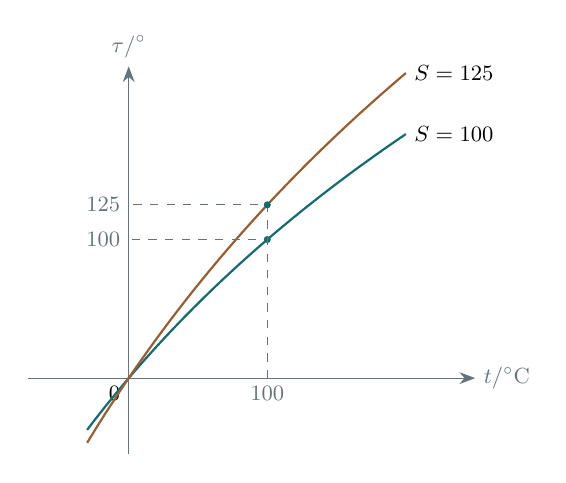
\begin{tikzpicture}[scale=.88,transform shape]
\draw[axis](-1.45,0)--(5,0)node[right]{$t/ ^\circ\mathrm C$};\draw[axis](0,-1.1)--(0,4.5)node[above]{$\tau/{}^\circ$};\node[below left]at(0,0){$0$};\draw[traj,domain=-.6:4,samples=70]plot(\x,{2*ln(1+50*\x/273.15)/ln(373.15/273.15)});\draw[force,-,domain=-.6:4,samples=70]plot(\x,{1.25*(2*ln(1+50*\x/273.15)/ln(373.15/273.15))});\draw[guide](2,0)node[below]{100}--(2,2)--(0,2)node[left]{100};\fill[accent](2,2)circle(1.45pt);\draw[guide](2,0)node[below]{}--(2,2.5)--(0,2.5)node[left]{125};\fill[accent](2,2.5)circle(1.45pt);\node[right]at(4,4.40){$S=125$};\node[right]at(4,3.52){$S=100$};
\end{tikzpicture}
\figcaption{变图 热1.1V6\quad 汽点读数提高后纵坐标按相同倍数伸长}
\end{minipage}\end{center}
新温标为$\tau_S=(S/100)\tau$，对$t>0$有$\tau_S>\tau$，对$t<0$有$\tau_S<\tau$。
对同一对实际温度端点，摄氏温差相同，读数差变为原来的 $S/100$ 倍。
变图 热1.1V6 取 $S=125$。冰点上方的读数随比例增大，冰点下方的负读数绝对值也增大，两曲线在零读数处相交。
\item 反求摄氏温度。
\begin{center}\begin{minipage}{.98\linewidth}\centering
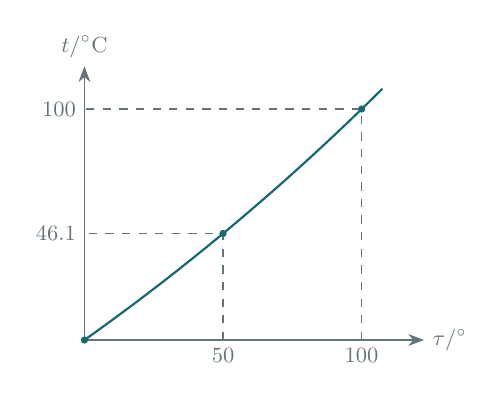
\begin{tikzpicture}[scale=.88,transform shape]
\draw[axis](0,0)--(4.9,0)node[right]{$\tau/{}^\circ$};\draw[axis](0,0)--(0,3.95)node[above]{$t/{}^\circ\mathrm C$};\draw[traj,domain=0:4.3,samples=65]plot(\x,{273.15*(exp(ln(373.15/273.15)*\x/4)-1)/30});\draw[guide](2,0)node[below]{50}--(2,1.53695)--(0,1.53695)node[left]{46.1};\draw[guide](4,0)node[below]{100}--(4,3.33333)--(0,3.33333)node[left]{100};\foreach \x/\y in {0/0,2/1.53695,4/3.33333}{\fill[accent](\x,\y)circle(1.5pt);}
\end{tikzpicture}
\figcaption{变图 热1.1V7\quad 以道尔顿读数为横坐标反求摄氏温度}
\end{minipage}\end{center}
由$A\tau=\ln(T/T_0)$得$T=T_0e^{A\tau}$，于是
\[
t=273.15\left[\left(\frac{373.15}{273.15}\right)^{\tau/100}-1\right].
\]
代$\tau=0,100$分别回到0、100℃；代$\tau=50$得到46.1084℃，与解图热1.1B的几何平均体积一致。
变图 热1.1V7 以 $\tau$ 为横坐标，先定位 $50$ 度，再向左读出 $46.1^\circ\mathrm C$；这就是解图热1.1B的中间体积所对应的温度。
\end{enumerate}

\clearpage

\pdfbookmark[2]{第 2 题 热电偶非线性电动势与自定温标}{q2}

\section*{第 2 题\quad 热电偶非线性电动势与自定温标}

热电偶的一个触点始终保持在$0^\circ\mathrm C$，另一个触点接触待测物体。待测温度为$t\,{}^\circ\mathrm C$时，热电动势为
\[\mathcal E=\alpha t+\beta t^2,\qquad
\alpha=0.20\,\mathrm{mV}/{}^\circ\mathrm C,\quad
\beta=-5.0\times10^{-4}\,\mathrm{mV}/({}^\circ\mathrm C)^2.\]
以$\mathcal E$为测温属性，定义$t^*=a\mathcal E+b$，并规定冰点$t^*=0^\circ$、汽点$t^*=100^\circ$。求$t^*(t)$，画出曲线，并讨论这一温标能否在整个温区唯一确定温度。

\begin{center}\begin{minipage}{0.96\linewidth}\centering
\begin{tikzpicture}[x=1cm,y=1cm]
\fill[warm!7] (-.35,.65) rectangle (.35,1.35);
\fill[accent!7] (2.05,.65) rectangle (2.75,1.35);
\draw[object] (0,1)--(0,2.2)--(4,2.2)--(4,1.4);
\draw[object] (4,.6)--(4,0)--(2.4,0)--(2.4,1);
\draw[very thick,warm] (0,1)--(2.4,1);
\fill (0,1) circle(2pt);\fill (2.4,1) circle(2pt);
\draw[object] (4,1) circle(.4);\node at (4,1) {$\mathcal E$};
\node[above] at (1.7,2.2) {金属$A$};
\node[above] at (1.2,1) {金属$B$};
\node[left,align=right] at (-.4,1) {$H$热端\\$t\,{}^\circ\mathrm C$};
\node[above,align=center] at (2.4,1.35) {$C$冷端\\$0^\circ\mathrm C$};
\node[below] at (2,-.35) {$\mathcal E=\alpha t+\beta t^2,\quad t^*=a\mathcal E+b$};
\end{tikzpicture}\figcaption{图 热1.2　热电动势与温标读数之间规定线性对应。}\end{minipage}\end{center}

\Needspace{5\baselineskip}

\pdfbookmark[3]{题型定位}{q2-h0}

\subsection*{题型定位}

把热电偶输出通过两点标定换为表盘读数，再用抛物线的单调支判断测温区间。读数的可逆性与顶点附近的灵敏度分开讨论。

\Needspace{5\baselineskip}

\pdfbookmark[3]{知识点}{q2-h1}

\subsection*{知识点}

冷端保持冰点，热电势 $\mathcal E(t)$ 为开口向下的二次函数。冰、汽两点确定纵轴的仿射变换。配方给顶点及两根，导数给单调性和灵敏度；校准偏差由 $t^*-t$ 求出，读数扰动可按局部导数传播。

\Needspace{5\baselineskip}

\pdfbookmark[3]{物理图像}{q2-h2}

\subsection*{物理图像}

图热1.2中，金属 $A,B$ 在 $H,C$ 相接。热端 $H$ 接触待测物体，冷端 $C$ 保持冰点。解图热1.2A中，$t^*=100$ 的水平线在顶点两侧各截一点，横坐标为100℃和300℃。顶点的水平切线使附近读数差随离顶点距离的平方改变。

\Needspace{5\baselineskip}

\pdfbookmark[3]{解题入口}{q2-h3}

\subsection*{解题入口}

先将冰点的0毫伏和汽点的15毫伏代入 $t^*=a\mathcal E+b$，求出纵轴的比例和零点。把读数函数配方后，再由工作温区选定反解所在的一支。

\Needspace{5\baselineskip}

\pdfbookmark[3]{标准解法}{q2-h4}

\subsection*{标准解法}

\textbf{固定点决定$a,b$。}冷端保持0℃，故冰点$\mathcal E(0)=0$，由$t^*(0)=0$得$b=0$。汽点的电动势为
\[\mathcal E(100)=0.20\times100-5.0\times10^{-4}\times100^2
=15.0\,\mathrm{mV}.\]
因此$100=a\times15.0$，即$a=20/3\,{}^\circ/\mathrm{mV}$。代回电动势关系，
\result{t^*=\frac43t-\frac{t^2}{300}
=\frac{400}{3}-\frac{(t-200)^2}{300}.}
\begin{center}\begin{minipage}{0.96\linewidth}\centering
\begin{tikzpicture}[x=1cm,y=1cm]
\draw[axis] (0,0)--(5.1,0) node[right] {$t/{}^\circ\mathrm C$};
\draw[axis] (0,-.25)--(0,3.2) node[above] {$t^*/{}^\circ$};
\draw[traj,domain=0:4,samples=90] plot (\x,{8*\x/3-2*\x*\x/3});
\draw[guide] (1,0) node[below]{100}--(1,2)--(0,2) node[left]{100};
\draw[guide] (2,0) node[below]{200}--(2,{8/3})--(0,{8/3}) node[left]{$400/3$};
\draw[guide] (3,0) node[below]{300}--(3,2)--(1,2);
\node[below] at (4,0) {400};\fill[accent] (2,{8/3}) circle(1.5pt);
\node[above right] at (2,{8/3}) {极大值};
\fill[accent] (1,2) circle(1.3pt);\fill[accent] (3,2) circle(1.3pt);
\end{tikzpicture}\figcaption{解图 热1.2A　200℃两侧各有一条单调支；相同读数可能对应两个温度。}\end{minipage}\end{center}
\textbf{曲线与测温区间。}解图热1.2A的抛物线开口向下，过$(0,0)$、$(100,100)$、$(400,0)$，顶点为$(200,400/3)$。导数
\[\frac{\dd t^*}{\dd t}=\frac43-\frac{t}{150}\]
在$t<200$时为正，在$t>200$时为负。单独使用一条单调支才能由$t^*$确定$t$。由配方式，
\[t=200\pm\sqrt{40000-300t^*}.\]
两个代数根具有明确的测温含义。例如$t^*=100$时，
\[t=200\pm\sqrt{40000-30000}=100\quad\hbox{或}\quad300.\]
两种实际温度给同一电动势读数；若已知只在0至100℃内测温，应选$t=100$。解图热1.2A中顶点两侧各是一条单调支，而在顶点$t=200$附近，实际温度变化引起的读数变化只从二阶开始，反求温度会非常敏感。

反函数的正负号由指定温区决定；顶点处一阶灵敏度为零。在冰点至汽点范围，$t^*$略大于$t$，其偏差为
\[t^*-t=\frac{t(100-t)}{300},\]
在$t=50^\circ\mathrm C$达到最大$25/3\approx8.33$度。两端偏差为零；中间各点的偏差来自二次项。
\subsubsection*{电动势、读数与反求温度的三步关系}
图热1.2中热端为接点$H$，冷端为接点$C$；电动势表接入回路，
接点 $C$ 保持 $0^\circ\mathrm C$ 时，表上的电势差由 $H$ 的温度 $t$ 决定。
先由两个固定点定出线性映射，再将电动势的二次规律代入：
\[
t^*=a(\alpha t+\beta t^2)+b,\qquad
0=a\mathcal E(0)+b,\qquad
100=a\mathcal E(100)+b.
\]
其中$a,b$由定标条件确定，$\alpha,\beta$则由热电偶的测量规律给出，
两组系数的作用不同。解图热1.2A的顶点还可直接从电动势求得：
\[
\frac{\dd\mathcal E}{\dd t}=\alpha+2\beta t=0
\ \Longrightarrow\ t_{\rm m}=200^\circ\mathrm C,\qquad
\mathcal E_{\max}=20.0\,\mathrm{mV}.
\]
乘以$a=20/3$得到$t^*_{\max}=400/3$，与配方结果一致。
抛物线的两零点是0℃与400℃，同一读数的两温度之和恒为400℃。
例如$t=100^\circ\mathrm C$和$300^\circ\mathrm C$都有$\mathcal E=15\,\mathrm{mV}$；
同一个15毫伏信号经过表盘的仿射映射，得到同一个读数。

在指定的$0\le t\le100$工作区，$0\le t^*\le100$且函数严格递增，
由此取顶点左侧的根
\[
t=200-\sqrt{40000-300t^*}.
\]
在 $t\ge200$ 的递减支上取正号。工作区若向顶点两侧延伸，从图上用一条略低于顶点的水平线便能截到两支。
在二次关系适用的温区内，抛物线的最大值为 $400/3$，更高读数对应的水平线位于曲线之上。

在任一单调支上，读数扰动远小于该点到峰值的读数差 $(t-200)^2/300$ 时，一阶误差传播给出
\[
\left|\frac{\dd t}{\dd t^*}\right|
=\frac{150}{|200-t|},\qquad
|\delta t|\simeq\frac{150|\delta t^*|}{|200-t|}.
\]
例如$t=100^\circ\mathrm C$附近，0.1度的读数小误差约对应0.15℃；
温度为 $199^\circ\mathrm C$ 时，读数离最大值只有 $1/300$ 度。若读数降低 $0.1$ 度，精确的峰值差为 $31/300$ 度，沿左支反解得 $t=200-\sqrt{31}\simeq194.43^\circ\mathrm C$，比原温度低约 $4.57^\circ\mathrm C$。
图中顶点切线水平，正是失去一阶灵敏度的几何表示。


\Needspace{5\baselineskip}

\pdfbookmark[3]{关键洞察}{q2-h5}

\subsection*{关键洞察}

等读数点关于 $t=200^\circ\mathrm C$ 对称，工作区限制在单调支后可以唯一反解。把工作点布置得远离顶点，读数对温度的响应更强。两点校准确定的是输出到读数的线性关系，中间的系统偏差还可用已知校准函数修正。

\Needspace{5\baselineskip}

\pdfbookmark[3]{易错点}{q2-h6}

\subsection*{易错点}

冰点和汽点分别以0、15毫伏代入。冷端偏离冰点时，模型写为热端电势函数与冷端电势函数之差。

$t^*=100$ 对应100℃与300℃，温区决定选根。读数极值在200℃，冰点至汽点的偏差极值在50℃。顶点附近的温度区间直接由精确的平方根关系求出。

\Needspace{5\baselineskip}

\pdfbookmark[3]{课堂讲解建议}{q2-h7}

\subsection*{课堂讲解建议}

先让学生在图热1.2上指出两个接点和仪表，再用两个已知温度确定 $a,b$。沿解图热1.2A的水平线从读数100找出两个温度，由题设工作区选根。

在199℃旁画出局部切线，比较0.1度读数变化与顶点读数差 $1/300$ 度，随后用平方根式解释切线近似的适用范围。另画变图热1.2V4中的偏差曲线，用两张图的纵轴解释为什么两个极值位置不同。


\Needspace{5\baselineskip}

\pdfbookmark[3]{变式训练}{q2-h8}

\subsection*{变式训练}

\begin{enumerate}
\item 仪表改读电动势的平方根。冰点仍给 $b=0$，汽点给 $a=100/\sqrt{15\,\mathrm{mV}}$，于是
\[
t^*=100\sqrt{\frac{\alpha t+\beta t^2}{15\,\mathrm{mV}}}.
\]
二次电势在 $0\le t\le400$ 时非负。变图热1.2V1的点 $A,B$ 分别为100℃、300℃，电势均为15毫伏，开方之后表盘仍读100度。将工作区取在0至100℃内，曲线严格递增，同一读数对应一个温度。
\begin{center}\begin{minipage}{.98\linewidth}\centering
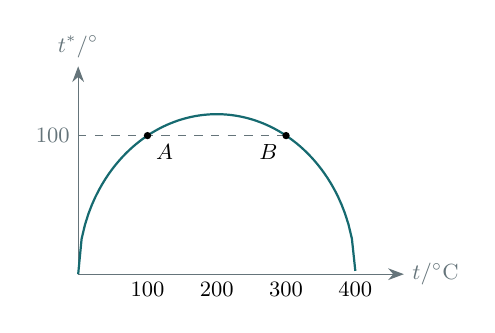
\begin{tikzpicture}[scale=.88,transform shape]
\draw[axis](0,0)--(4.7,0)node[right]{$t/{}^\circ\mathrm C$};\draw[axis](0,0)--(0,3.0)node[above]{$t^*/{}^\circ$};\draw[traj,domain=0:4,samples=82]plot(\x,{2*sqrt(max(0,(20*\x-5*\x*\x)/15))});\node[below]at(1,0){100};\node[below]at(2,0){200};\node[below]at(3,0){300};\node[below]at(4,0){400};\draw[guide](0,2)node[left]{100}--(3,2);\fill(1,2)circle(1.5pt)node[below right]{$A$};\fill(3,2)circle(1.5pt)node[below left]{$B$};
\end{tikzpicture}
\figcaption{变图 热1.2V1\quad 开方后保留相同电势的两个温度点}
\end{minipage}\end{center}
\item 若 $\mathcal E=c_1t+c_2t^2+c_3t^3$，冰点自动给 $\mathcal E(0)=0$。若已知汽点电势为 $E_s$，三个传感器系数只满足一个约束 $100c_1+10^4c_2+10^6c_3=E_s$。变图热1.2V2给出同一冰、汽点的两条可能曲线，按 $u=t/100$ 写成 $\mathcal E/E_s=u$ 与 $u+0.6u^2(1-u)$。若三系数已由独立测量给定且 $E_s\ne0$，两点刻度给 $b=0,a=100/E_s$。读数导数为
\[
\frac{\dd t^*}{\dd t}=\frac{100}{E_s}(c_1+2c_2t+3c_3t^2),
\]
在工作区依据它的符号选取单调支。
\begin{center}\begin{minipage}{.98\linewidth}\centering
\begin{tikzpicture}[scale=.88,transform shape]
\draw[axis](0,0)--(5,0)node[right]{$u$};\draw[axis](0,0)--(0,3.65)node[above]{$\mathcal E/E_s$};\draw[guide,domain=0:4,samples=82]plot(\x,{3*\x/4});\draw[traj,domain=0:4,samples=82]plot(\x,{3*(\x/4+.6*(\x/4)^2*(1-\x/4))});\node[below]at(4,0){1};\draw[guide](0,3)node[left]{1}--(4,3);\fill(4,3)circle(1.4pt);\node[right]at(1.75,1.76){三次函数};\node[below right]at(2.6,1.93){一次函数};
\end{tikzpicture}
\figcaption{变图 热1.2V2\quad 两固定点相同，点间的三次电势曲线仍可不同}
\end{minipage}\end{center}
\item 在工作区 $0\le t\le100$，令 $s=\dd t^*/\dd t=4/3-t/150$。变图热1.2V3的直线从冰点的 $4/3$ 下降至汽点的 $2/3$，同样小的温升在冰点附近引起约两倍的读数变化。比较速率的大小时取 $|s|$，例如在200℃以上的形式二次模型中，$|s|=(t-200)/150$ 随 $t$ 增加，向无限温度外推时无界。
\begin{center}\begin{minipage}{.98\linewidth}\centering
\begin{tikzpicture}[scale=.88,transform shape]
\draw[axis](0,0)--(5,0)node[right]{$t/{}^\circ\mathrm C$};\draw[axis](0,0)--(0,3.0)node[above]{$s$};\draw[traj](0,{8/3})node[left]{$4/3$}--(4,{4/3});\draw[guide](4,0)node[below]{100}--(4,{4/3})--(0,{4/3})node[left]{$2/3$};
\end{tikzpicture}
\figcaption{变图 热1.2V3\quad 冰点到汽点的表盘灵敏度}
\end{minipage}\end{center}
\item 冰点与汽点之间的偏差为 $\Delta=t^*-t=t(100-t)/300$。求导得 $\Delta'=1/3-t/150$，在50℃处为零，且 $\Delta''=-1/150$。变图热1.2V4中，偏差曲线两端为零，顶点为 $(50,25/3)$，故这一标定区间的最大偏差为 $25/3$ 度。超出该区间时，由二次式在新的温区分别求偏差的大小。
\begin{center}\begin{minipage}{.98\linewidth}\centering
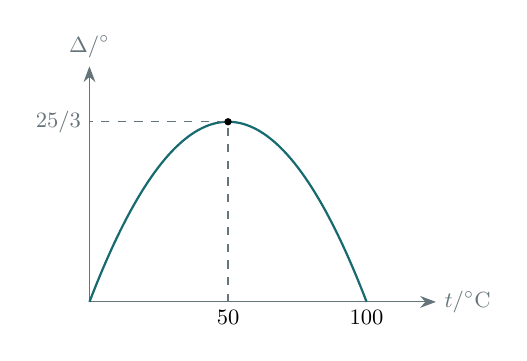
\begin{tikzpicture}[scale=.88,transform shape]
\draw[axis](0,0)--(5,0)node[right]{$t/{}^\circ\mathrm C$};\draw[axis](0,0)--(0,3.4)node[above]{$\Delta/{}^\circ$};\draw[traj,domain=0:4,samples=82]plot(\x,{\x*(4-\x)*.65});\node[below]at(2,0){50};\node[below]at(4,0){100};\draw[guide](2,0)--(2,2.6)--(0,2.6)node[left]{$25/3$};\fill(2,2.6)circle(1.5pt);
\end{tikzpicture}
\figcaption{变图 热1.2V4\quad 冰汽点之间的最大刻度偏差在50摄氏度}
\end{minipage}\end{center}
\item 冷端改为恒温 $t_c$，采用 $\mathcal E_c=f(t)-f(t_c)$，其中 $f(t)=\alpha t+\beta t^2$。变图热1.2V5取 $t_c=20^\circ\mathrm C$，故 $f(t_c)=3.8\,\mathrm{mV}$，两条电势曲线相差相同的纵向距离。重新定标写成
\[
0=-af(t_c)+b,\qquad 100=a[15\,\mathrm{mV}-f(t_c)]+b.
\]
相减得 $a=100/(15\,\mathrm{mV})$，再得 $b=af(t_c)$。代回有 $t^*=af(t)$。若刻度保留 $b=0$，所有读数便同时减少 $af(t_c)$。
\begin{center}\begin{minipage}{.98\linewidth}\centering
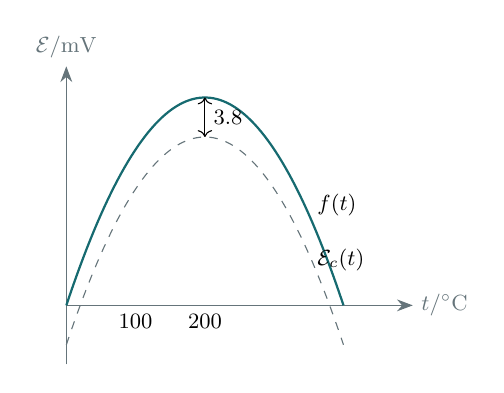
\begin{tikzpicture}[scale=.88,transform shape]
\draw[axis](0,0)--(5,0)node[right]{$t/{}^\circ\mathrm C$};\draw[axis](0,-.85)--(0,3.45)node[above]{$\mathcal E/\mathrm{mV}$};\draw[traj,domain=0:4,samples=82]plot(\x,{.15*(20*\x-5*\x*\x)});\draw[guide,domain=0:4,samples=82]plot(\x,{.15*(20*\x-5*\x*\x-3.8)});\node[below]at(1,0){100};\node[below]at(2,0){200};\draw[<->](2,2.43)--(2,3)node[midway,right]{3.8};\node[right]at(3.5,1.45){$f(t)$};\node[right]at(3.5,.66){$\mathcal E_c(t)$};
\end{tikzpicture}
\figcaption{变图 热1.2V5\quad 冷端保持20摄氏度时，两条电势曲线相差3.8毫伏}
\end{minipage}\end{center}
\item 当 $\beta=0,\alpha\ne0$，冰点仍给 $b=0$，汽点给 $100=a\alpha\,100$，因此 $a=1/\alpha$，从而 $t^*=t$。变图热1.2V6的直线贯穿两固定点，斜率恒为1；在传感器服从这一线性模型的温区，每个读数只对应一个温度。虚线标出二次模型在相同温区的曲率。
\begin{center}\begin{minipage}{.98\linewidth}\centering
\begin{tikzpicture}[scale=.88,transform shape]
\draw[axis](0,0)--(5,0)node[right]{$t/{}^\circ\mathrm C$};\draw[axis](0,0)--(0,4.5)node[above]{$t^*/{}^\circ$};\draw[traj,domain=0:4,samples=82]plot(\x,{\x});\draw[guide,domain=0:4,samples=82]plot(\x,{4*\x/3-\x*\x/12});\node[below]at(4,0){100};\draw[guide](0,4)node[left]{100}--(4,4);\node at(2.4,1.39){线性电势};\node at(1.95,3.01){二次电势};
\end{tikzpicture}
\figcaption{变图 热1.2V6\quad 线性传感器定标后读数与摄氏数值一致}
\end{minipage}\end{center}
\item 表盘读100度时，$t^2-400t+30000=0$ 的根为100℃和300℃，两者均对应15毫伏。变图热1.2V7把两条单调支分别画为不同线型。工作区为 $0\le t\le100$ 时，取左支的100℃；工作区在200℃以上时，取右支的300℃。若整个区间跨过这两个点，精确的电势值也给出同一对根。
\begin{center}\begin{minipage}{.98\linewidth}\centering
\begin{tikzpicture}[scale=.88,transform shape]
\draw[axis](0,0)--(5,0)node[right]{$t/{}^\circ\mathrm C$};\draw[axis](0,0)--(0,3.5)node[above]{$t^*/{}^\circ$};\draw[traj,domain=0:2,samples=82]plot(\x,{8*\x/3-2*\x*\x/3});\draw[traj,dashed,domain=2:4,samples=82]plot(\x,{8*\x/3-2*\x*\x/3});\node[below]at(1,0){100};\node[below]at(2,0){200};\node[below]at(3,0){300};\draw[guide](0,2)node[left]{100}--(3,2)--(3,0);\draw[guide](1,0)--(1,2);\fill(1,2)circle(1.6pt);\fill(3,2)circle(1.6pt);\node[above]at(1.15,2.67){左支};\node[above]at(3.48,2.25){右支};
\end{tikzpicture}
\figcaption{变图 热1.2V7\quad 同一百刻度水平线在顶点两侧各有一个交点}
\end{minipage}\end{center}
\end{enumerate}

\Needspace{18\baselineskip}

\pdfbookmark[2]{第 3 题 多只贮气罐给真空室逐次充气}{q3}

\section*{第 3 题\quad 多只贮气罐给真空室逐次充气}

每个贮气罐体积为$V$，初始压强为$p$。将一罐接到体积为$V_0$的真空室，开阀达到平衡后关阀，再换一只新的同样的罐继续充气，如此反复。全程温度不变。要使室内压强达到或超过$p_0$（$0<p_0<p$），至少需要多少罐？若最后一次允许提前关阀，说明怎样恰好达到$p_0$。

\begin{center}\begin{minipage}{0.96\linewidth}\centering
\begin{tikzpicture}[x=1cm,y=1cm]
\draw[object,fill=accent!7] (0,0) rectangle (2,2);\node[align=center] at (1,1) {新罐\\$V,p$};
\draw[object] (2,1)--(3,1);\draw[object] (2.45,.8)--(2.55,1.2);\node[above] at (2.5,1.25) {阀};
\draw[object,fill=accent!7] (3,0) rectangle (6,2);\node[align=center] at (4.5,1) {气室\\$V_0,p_{k-1}$};
\draw[motion] (2.1,.5)--(2.9,.5);
\end{tikzpicture}\figcaption{图 热1.3　每次接入新罐，关阀后保留气室中的气体。}\end{minipage}\end{center}

\Needspace{5\baselineskip}

\pdfbookmark[3]{题型定位}{q3-h0}

\subsection*{题型定位}

等温条件下的分轮充气。一次连接确定一次气体分配，关阀后气室内的部分进入下一轮，按压强目标求最小整数罐数。

\Needspace{5\baselineskip}

\pdfbookmark[3]{知识点}{q3-h1}

\subsection*{知识点}

等温条件下 $pV= nRT$，连通的罐和气室在达到平衡前合计摩尔数守恒。平衡时按容积比分配。气室相对供气压强 $p$ 的差值是一列公比 $r=V_0/(V+V_0)$ 的等比数列。

\Needspace{5\baselineskip}

\pdfbookmark[3]{物理图像}{q3-h2}

\subsection*{物理图像}

图热1.3左侧的罐每次换新，右侧气室保留关阀时所含的气体。解图热1.3A的虚线给供气压强，点列给完全平衡后的室压。目标在两个点之间时，末罐提前关阀，罐压仍高于室压。

\Needspace{5\baselineskip}

\pdfbookmark[3]{解题入口}{q3-h3}

\subsection*{解题入口}

写出 $p_k(V+V_0)=pV+V_0p_{k-1}$。把每个 $p_k$ 与同一个 $p$ 作差，得到 $p-p_k=r(p-p_{k-1})$，继而求压差通项。对照目标压强比找达到目标的第一个整数 $k$。

\Needspace{5\baselineskip}

\pdfbookmark[3]{标准解法}{q3-h4}

\subsection*{标准解法}

\textbf{每次平衡时气体如何分配。}图热1.3中每次接入的是新罐；旧罐剩余气体随罐移走。令
\[n=\frac{pV}{RT},\qquad r=\frac{V_0}{V_0+V},\qquad 0<r<1.\]
相同温度和压强下，两容器内摩尔数之比就是体积比。第一次平衡后
\[p_1=\frac{nRT}{V_0+V}=(1-r)p,\qquad n_1=rn.\]
第二次接入总摩尔数$n+n_1$，因此
\[p_2=\frac{(n+n_1)RT}{V_0+V}=(1+r)(1-r)p,\quad
n_2=r(n+n_1)=r(1+r)n.\]
第三次同理，
\[p_3=(1+r+r^2)(1-r)p,\qquad n_3=r(1+r+r^2)n.\]
从这三次分配可以看出，一般有
\begin{align*}
p_k&=(1+r+\cdots+r^{k-1})(1-r)p=(1-r^k)p,\\
n_k&=r(1+r+\cdots+r^{k-1})n
=\frac{r(1-r^k)}{1-r}n=\frac{V_0p_k}{RT}.
\end{align*}
\Needspace{26\baselineskip}\textbf{每次开阀后的压强递推。}第 $k$ 次开阀前，两容器的总摩尔数为 $(pV+V_0p_{k-1})/(RT)$。平衡后气体充满总体积 $V+V_0$，因此
\[p_k=\frac{pV+V_0p_{k-1}}{V+V_0},\qquad
p-p_k=r(p-p_{k-1}).\]
\begin{center}\begin{minipage}{0.96\linewidth}\centering
\begin{tikzpicture}[x=1cm,y=1cm]\draw[axis] (0,0)--(6,0) node[right] {$k$};\draw[axis] (0,0)--(0,2.7) node[above] {$p_k/p$};

\draw[guide] (0,2.2) node[left]{1}--(5.6,2.2);
\foreach \k in {0,...,8}{\fill[accent] ({.65*\k},{2.2*(1-pow(.65,\k))}) circle(1.6pt);}
\foreach \k in {0,2,4,6,8}{\node[below] at ({.65*\k},0) {$\k$};}
\node[align=left] at (3.7,.6) {$p-p_k=r^k p$\\示意取$r=0.65$};
\end{tikzpicture}\figcaption{解图 热1.3A　达到平衡后的压强呈离散增长，压强差按等比数列衰减。}\end{minipage}\end{center}
解图热1.3A中压强一直增加，但每个有限次的点与供气压强仍差 $r^kp>0$。要求$p_k\ge p_0$等价于
\[r^k\le1-\frac{p_0}{p}.
\]
$0<r<1$，故除以负数 $\ln r$ 后取满足下界的最小整数。
\result{K_{\min}=\left\lceil\frac{\ln(1-p_0/p)}{\ln[V_0/(V_0+V)]}\right\rceil.}
阈值为整数时，末罐完全平衡恰达目标。阈值有小数时，末罐完全平衡后超过目标。允许提前关阀时，第$K$罐充气过程中室压由低于$p_0$升至不低于$p_0$，在达到$p_0$时关阀即可。目标 $p_0=0$ 对应初态；有限次充气所得压强均低于 $p$。
\subsubsection*{守恒式、最少罐数与末罐余气}
图热1.3中每轮开阀时，系统只包括新罐和气室；关阀移走旧罐后，下一轮只保留气室内的气体。
令第$k$次平衡后移走的罐中摩尔数为$m_k$，则
\[
n+n_{k-1}=n_k+m_k,\qquad
n_k=\frac{V_0p_k}{RT},\qquad m_k=\frac{Vp_k}{RT}.
\]
两容器温度及平衡压强相同，所以$n_k/m_k=V_0/V$。
把这一分配关系代入守恒式，得$n_k=r(n+n_{k-1})$；
初值$n_0=0$逐次产生$n_1=rn,n_2=r(1+r)n,n_3=r(1+r+r^2)n$，
再由等比和得到已经写出的通项。每轮实际进入气室的摩尔数因而逐次减小。

从压强差式还可求每轮增量：
\[
p_k-p_{k-1}=(1-r)r^{k-1}p>0,\qquad
n_k-n_{k-1}=\frac{V_0}{RT}(1-r)r^{k-1}p.
\]
解图热1.3A中相邻离散点的高度差越来越小，正对应这里的$r^{k-1}$。
图中用 $r=0.65$ 作示例；由具体容积求得的 $r$ 决定各点的高度。

记实数阈值
\[
K_*=\frac{\ln(1-p_0/p)}{\ln r}.
\]
若$K_*$恰为整数，完全平衡后可恰得$p_0$。
否则$K=\lceil K_*\rceil$满足
\[
p_{K-1}<p_0<p_K.
\]
因此$K$罐足够，$K-1$罐不足。数值计算中遇到接近整数的阈值，可把相邻的整数代回 $1-r^k$，直接比较室压和目标。

在末罐允许提前关阀时，令气室达到$p_0$的一刻新罐压强为$p_s$。
这次连接前气室压强为$p_{K-1}$，等温物质量守恒给出
\[
pV+p_{K-1}V_0=p_sV+p_0V_0,\qquad
p_s=p-\frac{V_0}{V}(p_0-p_{K-1}).
\]
由$p_K\ge p_0$等价得到$p_s\ge p_0$；
严格超出时$p_s>p_0$，关阀前仍有从罐流向气室的压差。
恰好平衡时才有 $p_s=p_0$。

各次余气量相加，得到移走的总摩尔数。$K$次均完全平衡时，移走的罐共带走
\[
\sum_{j=1}^K m_j
=n\left[K-\frac{r(1-r^K)}{1-r}\right],
\qquad
n_K=n\frac{r(1-r^K)}{1-r}.
\]
两式相加为$Kn$，与投入的总摩尔数一致。目标越接近$p$，
新增气室压强越小，每罐移走时的压强更接近初压 $p$，因而带走更大比例的气体。


\Needspace{5\baselineskip}

\pdfbookmark[3]{关键洞察}{q3-h5}

\subsection*{关键洞察}

每次平衡后有一部分气体留在左罐，使室压的增量随剩余压差一起缩小。平衡结果是一列离散值；末罐充气时，阀门可以在达到其中两个值之间的任一可达室压时关闭。

\Needspace{5\baselineskip}

\pdfbookmark[3]{易错点}{q3-h6}

\subsection*{易错点}

本轮平衡包含新罐和气室，下一轮初态只带入气室的摩尔数。随每轮推移，气室容积保持 $V_0$。

除以 $\ln r<0$ 后，罐数有一个实数下界，最少罐数取不小于它的整数。恰好在两个离散室压之间的目标由提前关阀达到，此时罐内压强由该轮摩尔数守恒求出。

\Needspace{5\baselineskip}

\pdfbookmark[3]{课堂讲解建议}{q3-h7}

\subsection*{课堂讲解建议}

按图热1.3做两轮，分别把左罐投入量、移走量和右侧气室保留量写在两边。由离散点列的高度差读出各轮室压增量，再用守恒式推到同一个公比。

在解图热1.3A选一条恰穿过点的目标线，再选一条落在相邻点之间的目标线。学生分别给出最少罐数与阀门时刻。在第二种情形用末罐余压公式说明，关闭阀门时气体仍有由罐流向气室的压差。


\Needspace{5\baselineskip}

\pdfbookmark[3]{变式训练}{q3-h8}

\subsection*{变式训练}

\begin{enumerate}
\item 各罐初压相同，容积按 $V_k$ 变化。把第 $k$ 轮的守恒式移项，有
\[
p-p_k=\frac{V_0}{V_0+V_k}(p-p_{k-1}),\qquad
p-p_K=(p-p_i)\prod_{k=1}^K\frac{V_0}{V_0+V_k}.
\]
变图热1.3V1取 $p_i=0$ 和 $V_k/V_0=1/4,1,1/3$，归一化压差依次从1变为 $0.8,0.4,0.3$，每一步由自己的容积比决定。目标高于 $p_i$ 时，找使乘积首次不大于 $(p-p_0)/(p-p_i)$ 的轮次。
\begin{center}\begin{minipage}{.98\linewidth}\centering
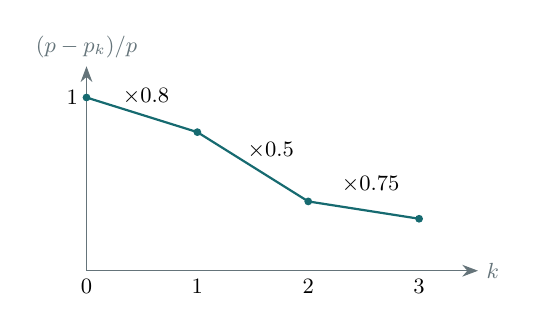
\begin{tikzpicture}[scale=.88,transform shape]
\draw[axis](0,0)--(5.65,0)node[right]{$k$};\draw[axis](0,0)--(0,2.95)node[above]{$(p-p_k)/p$};\draw[traj](0,2.5)--(1.6,2)--(3.2,1)--(4.8,.75);\fill[accent](0.0000,2.500000)circle(1.6pt);\node[below]at(0.0000,0){0};\fill[accent](1.6000,2.000000)circle(1.6pt);\node[below]at(1.6000,0){1};\fill[accent](3.2000,1.000000)circle(1.6pt);\node[below]at(3.2000,0){2};\fill[accent](4.8000,0.750000)circle(1.6pt);\node[below]at(4.8000,0){3};\node[left]at(0,2.5){1};\node[above]at(.86,2.28){$\times0.8$};\node[above right]at(2.2,1.50){$\times0.5$};\node[above]at(4.10,1.0){$\times0.75$};
\end{tikzpicture}
\figcaption{变图 热1.3V1\quad 变容积罐依次给出各轮的压差比例}
\end{minipage}\end{center}
\item 气室已有初压 $p_i<p$ 时，初始差值为 $p-p_i$，所以 $p_k=p-(p-p_i)r^k$。若 $p_i<p_0<p$，解得
\[
K=\left\lceil\frac{\ln[(p-p_0)/(p-p_i)]}{\ln r}\right\rceil .
\]
变图热1.3V2取 $r=0.65$、目标 $0.75p$，圆点从 $p_i/p=0.25$ 出发并在第3次越过目标；浅色点从真空出发，第4次越过。目标在初压或以下时取零罐；每次只消去现有压差的一部分，所以有限次所达室压仍在供气压强之下。
\begin{center}\begin{minipage}{.98\linewidth}\centering
\begin{tikzpicture}[scale=.88,transform shape]
\draw[axis](0,0)--(5.65,0)node[right]{$k$};\draw[axis](0,0)--(0,2.95)node[above]{$p_k/p$};\draw[guide](0,1.875)node[left]{.75}--(5.3,1.875);\fill[accent](0.0000,0.625000)circle(1.6pt);\node[below]at(0.0000,0){0};\fill[accent](0.8800,1.281250)circle(1.6pt);\node[below]at(0.8800,0){1};\fill[accent](1.7600,1.707812)circle(1.6pt);\node[below]at(1.7600,0){2};\fill[accent](2.6400,1.985078)circle(1.6pt);\node[below]at(2.6400,0){3};\fill[accent](3.5200,2.165301)circle(1.6pt);\node[below]at(3.5200,0){4};\fill[accent](4.4000,2.282446)circle(1.6pt);\node[below]at(4.4000,0){5};\fill[warm](0.0000,0.000000)circle(1.6pt);\fill[warm](0.8800,0.875000)circle(1.6pt);\fill[warm](1.7600,1.443750)circle(1.6pt);\fill[warm](2.6400,1.813438)circle(1.6pt);\fill[warm](3.5200,2.053734)circle(1.6pt);\fill[warm](4.4000,2.209927)circle(1.6pt);\node[left]at(0,.625){.25};\node[above right]at(3.55,2.45){有初压};\node[below right]at(3.30,1.50){初态真空};
\end{tikzpicture}
\figcaption{变图 热1.3V2\quad 从非零初压和真空出发的两组点列}
\end{minipage}\end{center}
\item 初态真空，目标是供气压的固定比例 $f$。把两边都除以 $p$，得到 $1-r^K\ge f$，最少轮次为
\[
K=\left\lceil\frac{\ln(1-f)}{\ln r}\right\rceil.
\]
变图热1.3V3中，供气压强从 $p$ 增为 $1.4p$，把室压和目标都用各自的供气压强归一化后，两组点完全重合。反过来，若绝对目标保持固定，其归一化高度会降低。要求恰好达到 $fp$ 时，末罐的罐压为 $p-(V_0/V)(fp-p_{K-1})$，室压达到 $fp$ 即关阀。
\begin{center}\begin{minipage}{.98\linewidth}\centering
\begin{tikzpicture}[scale=.88,transform shape]
\draw[axis](0,0)--(5.65,0)node[right]{$k$};\draw[axis](0,0)--(0,2.95)node[above]{归一化室压};\draw[guide](0,1.875)node[left]{$f$}--(5.3,1.875);\fill[accent](0.0000,0.000000)circle(1.6pt);\node[below]at(0.0000,0){0};\fill[accent](0.8000,0.875000)circle(1.6pt);\node[below]at(0.8000,0){1};\fill[accent](1.6000,1.443750)circle(1.6pt);\node[below]at(1.6000,0){2};\fill[accent](2.4000,1.813438)circle(1.6pt);\node[below]at(2.4000,0){3};\fill[accent](3.2000,2.053734)circle(1.6pt);\node[below]at(3.2000,0){4};\fill[accent](4.0000,2.209927)circle(1.6pt);\node[below]at(4.0000,0){5};\foreach \j in {0,...,5}{\draw[warm,thin]({.8*\j},{2.5*(1-pow(.65,\j))})circle(2.9pt);}\node[right,align=left]at(2.35,.65){圆心：供气压$p$\\圆圈：供气压$1.4p$};
\end{tikzpicture}
\figcaption{变图 热1.3V3\quad 目标保持固定比例时，两组归一化室压点重合}
\end{minipage}\end{center}
\item 目标为 $0.9p$，通式给 $K=\lceil\ln0.1/\ln r\rceil$。变图热1.3V4用 $r=0.65$ 作例，第5次的 $p_5/p=0.883971<0.9$，第6次的 $p_6/p=0.924581>0.9$，故最少用6罐。固定 $V$ 而增大 $V_0$，$r$ 随之增大，每个 $p_k/p=1-r^k$ 降低，达到同一目标的罐数只会保持或增加。
\begin{center}\begin{minipage}{.98\linewidth}\centering
\begin{tikzpicture}[scale=.88,transform shape]
\draw[axis](0,0)--(6,0)node[right]{$k$};\draw[axis](0,0)--(0,3.15)node[above]{$p_k/p$};\draw[guide](0,2.25)node[left]{.90}--(5.7,2.25);\fill[accent](0.0000,0.000000)circle(1.6pt);\node[below]at(0.0000,0){0};\fill[accent](0.7600,0.875000)circle(1.6pt);\node[below]at(0.7600,0){1};\fill[accent](1.5200,1.443750)circle(1.6pt);\node[below]at(1.5200,0){2};\fill[accent](2.2800,1.813438)circle(1.6pt);\node[below]at(2.2800,0){3};\fill[accent](3.0400,2.053734)circle(1.6pt);\node[below]at(3.0400,0){4};\fill[accent](3.8000,2.209927)circle(1.6pt);\node[below]at(3.8000,0){5};\fill[accent](4.5600,2.311453)circle(1.6pt);\node[below]at(4.5600,0){6};\fill[accent](5.3200,2.377444)circle(1.6pt);\node[below]at(5.3200,0){7};\node[below left]at(3.8,2.21){.883971};\node[above right]at(4.56,2.31){.924581};
\end{tikzpicture}
\figcaption{变图 热1.3V4\quad 第5次低于目标，第6次越过目标}
\end{minipage}\end{center}
\item 重新接回第 $j<k$ 次用过的一罐。罐压仍为 $p_j$，小于气室的 $p_k$，变图热1.3V5中箭头由气室指向旧罐。平衡时两边共用
\[
p'=\frac{V_0p_k+Vp_j}{V_0+V},
\]
即 $p_j<p'<p_k$。若从第一罐开始让所有旧罐保持连通，图中右侧是另一种接法，气体量为 $KpV/(RT)$，容积为 $V_0+KV$，给 $p_K=pKV/(V_0+KV)$。它随 $K$ 增长所对应的剩余压差按 $1/(1+KV/V_0)$ 衰减。
\begin{center}\begin{minipage}{.98\linewidth}\centering
\begin{tikzpicture}[scale=.88,transform shape]
\draw[object](0,0)rectangle(1.3,1.4)node[midway,align=center]{旧罐\\$p_j$};\draw[object](2.36,0)rectangle(3.70,1.4)node[midway,align=center]{气室\\$p_k$};\draw[object](1.3,.7)--(2.36,.7);\draw[motion](2.25,1.07)--(1.38,1.07);\node at(1.85,-.55){重新接入一罐};\begin{scope}[xshift=4.4cm]\draw[object](0,0)rectangle(1.3,1.4)node[midway]{气室};\draw[object](1.3,.7)--(2.65,.7);\foreach \y in {-.33,.7,1.73}{\draw[object](2.46,{\y-.38})rectangle(3.22,{\y+.38});\draw[object](2.46,\y)--(1.91,\y)--(1.91,.7);}\node at(2.84,.7){罐};\node at(1.70,-1.00){各罐常连};\end{scope}
\end{tikzpicture}
\figcaption{变图 热1.3V5\quad 重新接入旧罐时回流；所有罐常连时容积随罐数增加}
\end{minipage}\end{center}
\item 保持绝对目标 $p_0$ 与容积比 $r$。用 $k$ 罐达标等价于
\[
p\ge p^{(k)}=\frac{p_0}{1-r^k}.
\]
变图热1.3V6取 $r=0.65$，横坐标为 $p/p_0$。横过 $1/(1-r^k)$ 时，最少罐数下降至 $k$，恰在台阶左端已经可以用 $k$ 罐。目标随供气压按固定比例变化时，$p_0/p$ 保持，最少罐数也保持。
\begin{center}\begin{minipage}{.98\linewidth}\centering
\begin{tikzpicture}[scale=.88,transform shape]
\draw[axis](0,0)--(5.8,0)node[right]{$p/p_0$};\draw[axis](0,0)--(0,3.2)node[above]{$K$};\draw[traj](4.45714,0.47)--(5.30000,0.47);\fill[accent](4.45714,0.47)circle(1.1pt);\draw[traj](1.75584,0.94)--(4.45714,0.94);\fill[accent](1.75584,0.94)circle(1.1pt);\draw[traj](0.90863,1.41)--(1.75584,1.41);\fill[accent](0.90863,1.41)circle(1.1pt);\draw[traj](0.52151,1.88)--(0.90863,1.88);\fill[accent](0.52151,1.88)circle(1.1pt);\draw[traj](0.31502,2.35)--(0.52151,2.35);\fill[accent](0.31502,2.35)circle(1.1pt);\draw[traj](0.19577,2.82)--(0.31502,2.82);\fill[accent](0.19577,2.82)circle(1.1pt);\node[below]at(0,0){1};\node[below]at(2.4,0){2};\node[below]at(4.8,0){3};\node[left]at(0,.47){1};\node[left]at(0,1.41){3};\node[left]at(0,2.35){5};
\foreach \xx/\yy in {4.45714/.94,1.75584/1.41,.90863/1.88,.52151/2.35,.31502/2.82}
  {\filldraw[fill=white,draw=accent] (\xx,\yy) circle(1.1pt);}
\end{tikzpicture}
\figcaption{变图 热1.3V6\quad 供气压提高时的最少罐数呈台阶下降}
\end{minipage}\end{center}
\item 小罐满足 $\varepsilon=V/V_0\ll1$，而 $r=(1+\varepsilon)^{-1}$。由 $\ln r=-\varepsilon+O(\varepsilon^2)$ 得
\[
K_*=\frac{-\ln(1-p_0/p)}{\ln(1+\varepsilon)}
\simeq\frac{V_0}{V}\ln\frac1{1-p_0/p}.
\]
求精确罐数时用左式再取上整。变图热1.3V7画的是首罐室压比 $\varepsilon/(1+\varepsilon)$，它随罐容积增大趋向1。与目标线相交处 $\varepsilon=p_0/(p-p_0)$，达到或超过这个容积比，一罐已足够。图中目标为 $0.8p$，交点对应 $\varepsilon=4$。
\begin{center}\begin{minipage}{.98\linewidth}\centering
\begin{tikzpicture}[scale=.88,transform shape]
\draw[axis](0,0)--(6.1,0)node[right]{$V/V_0$};\draw[axis](0,0)--(0,3.0)node[above]{$p_1/p$};\draw[guide](0,2.0)node[left]{.8}--(5.75,2.0);\draw[traj,domain=0:5.65,samples=85]plot(\x,{2.5*\x/(1+\x)});\draw[guide](4,0)node[below]{4}--(4,2);\fill[accent](4,2)circle(1.5pt);
\end{tikzpicture}
\figcaption{变图 热1.3V7\quad 大型贮罐的首轮室压与目标的交点}
\end{minipage}\end{center}
\end{enumerate}

\clearpage

\pdfbookmark[2]{第 4 题 U形管注入水银后的封闭气体压强}{q4}

\section*{第 4 题\quad U形管注入水银后的封闭气体压强}

截面均匀、两端等高的U形管竖直放置，内盛水。左端封闭，右端开口；初始左、右水面到管顶的距离分别为$h_1=30\,\mathrm{cm}$、$h_2=20\,\mathrm{cm}$。右水面上有质量可忽略、无摩擦且不漏气的薄活塞。在活塞上缓慢加入高$H=7.5\,\mathrm{cm}$的水银柱，其上表面恰与左水面等高。温度和外界压强$p_0$不变，水银密度为水的13.6倍。求$p_0$。

\begin{center}\begin{minipage}{0.96\linewidth}\centering
\begin{tikzpicture}[x=1cm,y=1cm]
\fill[accent!16] (0,0) rectangle(.7,1.2);\fill[accent!16] (2,0) rectangle(2.7,2.2);
\fill[accent!16] (0,0) rectangle(2.7,.4);
\draw[object] (0,4.2)--(0,0)--(2.7,0)--(2.7,4.2);
\draw[object] (.7,4.2)--(.7,.4)--(2,.4)--(2,4.2);\draw[object] (0,4.2)--(.7,4.2);
\draw[object,line width=2pt] (2,2.2)--(2.7,2.2);
\draw[guide] (0,4.2)--(3.1,4.2);
\draw[<->] (-.35,1.2)--(-.35,4.2) node[midway,left]{$h_1$};
\draw[<->] (3.1,2.2)--(3.1,4.2) node[midway,right]{$h_2$};
\node at (.35,2.7) {气};\node at (1.4,.15) {水};\node at (2.35,3.1) {$p_0$};
\node[below,align=center] at (1.35,-.25) {同一长度比例：$h_1:h_2=30:20$};
\end{tikzpicture}\figcaption{图 热1.4　初始两水面的高度差决定封闭气体的初压。}\end{minipage}\end{center}

\Needspace{5\baselineskip}

\pdfbookmark[3]{题型定位}{q4-h0}

\subsection*{题型定位}

连通液柱的静压、等截面水量守恒和封闭气体等温式联立。沿初态及末态各自的液柱求气压，再由几何确定气柱长度。

\Needspace{5\baselineskip}

\pdfbookmark[3]{知识点}{q4-h1}

\subsection*{知识点}

液体中每下降高度 $\Delta h$，压强增加 $\rho g\Delta h$。连通水中同高点等压。轻薄、无摩擦的活塞把液体隔开，活塞上下表面压强相等。封闭理想气体定温时，绝对压强与体积之积恒定。

\Needspace{5\baselineskip}

\pdfbookmark[3]{物理图像}{q4-h2}

\subsection*{物理图像}

图热1.4中左水面较低，封闭气压比大气压高10厘米水柱。解图热1.4A中的上水平线经过左水面 $L$ 与汞上表面 $R$，下水平线经过水中一点 $A$ 和活塞处 $B$。水量守恒使左水面升高8.75厘米、右活塞下降8.75厘米，左气柱末长21.25厘米。

\Needspace{5\baselineskip}

\pdfbookmark[3]{解题入口}{q4-h3}

\subsection*{解题入口}

由初态高差求 $p_i=p_0+\rho_wg(h_1-h_2)$。末态分别从 $L,R$ 下行到水中同高的 $A,B$，再令 $p_A=p_B$。设左升右降皆为 $u$，用 $h_1-u=h_2+u-H$ 求气柱末长，代入 $p_ih_1=p_fL_f$。

\Needspace{5\baselineskip}

\pdfbookmark[3]{标准解法}{q4-h4}

\subsection*{标准解法}

\textbf{先求两状态的压强。}图热1.4中右水面比左水面高$h_1-h_2$。沿同一种水向下到左水面的水平高度，压强增加，故初态
\[p_i=p_0+\rho_wg(h_1-h_2).\]
\begin{center}\begin{minipage}{0.96\linewidth}\centering
\begin{tikzpicture}[x=1cm,y=1cm]
\fill[accent!16] (0,0) rectangle(.7,2.075);\fill[accent!16] (2,0) rectangle(2.7,1.325);
\fill[accent!16] (0,0) rectangle(2.7,.4);
\fill[warm!35] (2,1.325) rectangle(2.7,2.075);
\draw[object] (0,4.2)--(0,0)--(2.7,0)--(2.7,4.2);
\draw[object] (.7,4.2)--(.7,.4)--(2,.4)--(2,4.2);\draw[object] (0,4.2)--(.7,4.2);
\draw[object,line width=2pt] (2,1.325)--(2.7,1.325);
\draw[guide] (0,2.075)--(3.2,2.075);\draw[guide] (0,1.325)--(3.2,1.325);
\draw[<->] (-.55,2.075)--(-.55,4.2) node[midway,left]{$L_f$};
\draw[<->] (3.2,1.325)--(3.2,2.075) node[midway,right]{$H$};
\fill (.35,1.325) circle(1.5pt);\node[below] at (.35,1.325) {$A$};
\node[below right] at (2.7,1.325) {$B$};
\node[left] at (0,2.075) {$L$};\node[right] at (2.7,2.075) {$R$};
\node at (2.35,1.7) {汞};\node at (.35,3.1) {$p_f$};\node at (1.4,.15) {水};
\node at (2.35,2.85) {$p_0$};
\node[below,align=center] at (1.35,-.25) {左水面升$u$，右活塞降$u$；$u=8.75\,\mathrm{cm}$};
\end{tikzpicture}\figcaption{解图 热1.4A　虚线分别经过左水面与右活塞；在活塞高度向左比较水压。}\end{minipage}\end{center}
在解图热1.4A中，从右水银上面向下到活塞，压强增加$\rho_{\rm Hg}gH$；再沿水回到左水面高度，压强减少$\rho_wgH$。活塞无重量，所以
\[p_f=p_0+(\rho_{\rm Hg}-\rho_w)gH.\]
\textbf{几何与体积守恒。}设左水面上升$u$。管截面相同，右水面及活塞下降$u$；右水银上面到管顶的距离为$h_2+u-H$。等高条件给出
\[h_1-u=h_2+u-H,\quad
u=\frac{H+h_1-h_2}{2}=8.75\,\mathrm{cm}.\]
故气柱末长
\[L_f=h_1-u=\frac{h_1+h_2-H}{2}=21.25\,\mathrm{cm}.\]
两侧的位移只由水量和管的等截面条件确定；密度比进入前面的液柱压强式。等温、封闭气体满足
\[[p_0+\rho_wg(h_1-h_2)]h_1
=[p_0+(\rho_{\rm Hg}-\rho_w)gH]L_f.\]
移项后
\[p_0=\rho_wg\,
\frac{12.6HL_f-(h_1-h_2)h_1}{h_1-L_f}.\]
\Needspace{16\baselineskip}\textbf{统一单位计算。}把全部几何长度改为毫米，设$p_0$的数值单位为mmHg，原式变为
\[\left(p_0+\frac{100}{13.6}\right)300
=\left(p_0+\frac{12.6\times75}{13.6}\right)212.5.\]
\result{p_0=143.54\,\mathrm{mmHg}\approx144\,\mathrm{mmHg}
\approx1.91\times10^4\,\mathrm{Pa}.}
按 $1\,\mathrm{atm}=101325\,\mathrm{Pa}=760\,\mathrm{mmHg}$ 换算，题中的大气压约为标准大气压的 $0.189$ 倍。
\subsubsection*{沿连通液体求静压与两侧气柱长度}
解图热1.4A以管顶为同一参考高度，初态左气柱30厘米、右水面深20厘米。
左水面升高8.75厘米后，末气柱长21.25厘米；
右活塞从深20厘米降到28.75厘米，水银上表面深度为$28.75-7.50=21.25$厘米。
图中的上方虚线经过左水面$L$和汞上表面$R$，下方虚线经过水内点$A$与活塞处$B$，
两线距离为$H$。两侧位移与两表面深度分别满足水量守恒和题设等高条件。

在右汞上表面$R$处为$p_0$，向下到$B$加$\rho_{\rm Hg}gH$；
左侧从$L$向下到$A$加$\rho_wgH$。$A,B$处于同一连通水体的同一高度，
且轻薄活塞两侧压强相同，故
\[
p_A=p_f+\rho_wgH,\qquad
p_B=p_0+\rho_{\rm Hg}gH,\qquad p_A=p_B.
\]
消去$p_A,p_B$便得$p_f=p_0+(\rho_{\rm Hg}-\rho_w)gH$。
从等高的 $L,R$ 各下行距离 $H$，压强增量分别为$\rho_wgH$和$\rho_{\rm Hg}gH$。水银密度较大，因此左侧气体压强$p_f$比$p_0$高出两液柱压强增量之差。

初末绝对压强约为
\[
p_i=150.892857\,\mathrm{mmHg},\qquad
p_f=213.025210\,\mathrm{mmHg},\qquad
\frac{p_f}{p_i}=\frac{30}{21.25}=\frac{24}{17}.
\]
该比值与气柱缩短的反比一致。若静压式先算出了表压，初、末两态都加上同一个 $p_0$，就得到上式所用的绝对压强。

为求出大气压强并确定其正值范围，记$\Delta=h_1-h_2$、$\sigma=\rho_{\rm Hg}/\rho_w$。
将$L_f=(h_1+h_2-H)/2$代入移项式，有
\[
\frac{p_0}{\rho_wg}
=\frac{(\sigma-1)H(h_1+h_2-H)-2h_1\Delta}{\Delta+H}.
\]
本题$\Delta+H>0$，分子也为正，给出压缩气体及正的大气压强。
代厘米长度得到水柱高度$p_0/(\rho_wg)=195.214286\,\mathrm{cm}$；
除13.6成为14.353992厘米汞柱，再乘10成为143.539916毫米汞柱。
密度比用于压强换算，厘米到毫米的十倍因子属于长度单位换算，两步的换算因子分别为13.6和10。


\Needspace{5\baselineskip}

\pdfbookmark[3]{关键洞察}{q4-h5}

\subsection*{关键洞察}

$A,B$ 等压的依据是经连通水达到同一高度。$L,R$ 到该水平线分别走过水柱和汞柱，压强增量之差为 $(\rho_{\rm Hg}-\rho_w)gH$。等温压缩给出 $p_f/p_i=30/21.25=24/17$，将它与静压关系联立即可反求大气压。

\Needspace{5\baselineskip}

\pdfbookmark[3]{易错点}{q4-h6}

\subsection*{易错点}

解图热1.4A中左水面和汞上表面对齐，右水面位于活塞下方。沿汞柱下降加静压，沿水柱上升减静压。等温式以绝对压强计算，位移则由水量守恒确定。用厘米长度算出的汞柱高度乘10才写成毫米汞柱。

用给定大气压反求汞高时，逐一把候选解的气柱长和活塞深度与管内几何比较。

\Needspace{5\baselineskip}

\pdfbookmark[3]{课堂讲解建议}{q4-h7}

\subsection*{课堂讲解建议}

在两幅图上以管顶为共同原点，用向下深度标出两界面，分别写初态和末态。沿解图热1.4A的 $L\to A$、$R\to B$ 路径标注液体和增压量，再由 $p_A=p_B$ 得到两上表面的压强差。换算 $195.214$ 厘米水柱时，先除密度比，再把厘米汞柱转成毫米汞柱。

把大气压设为已求值，沿变图热1.4V3找出两个汞柱高度。分别算两候选态的活塞位置，讨论底部深度怎样约束可取的状态。


\Needspace{5\baselineskip}

\pdfbookmark[3]{变式训练}{q4-h8}

\subsection*{变式训练}

\begin{enumerate}
\item 上液密度改为 $\sigma\rho_w$，其他几何条件保持。水量守恒仍给 $L_f=(h_1+h_2-H)/2$，变图热1.4V1的两条水平线相差 $H$。按左水右液分别求压强增量，得 $p_f=p_0+(\sigma-1)\rho_wgH$。等温式给
\[
\frac{p_0}{\rho_wg}
=\frac{(\sigma-1)HL_f-(h_1-h_2)h_1}{h_1-L_f}.
\]
气柱为压缩态时，正的大气压要求 $\sigma>1+(h_1-h_2)h_1/(HL_f)$，本题几何对应 $\sigma>2.8824$。所求液面需处于管内，并留出 $L_f>0$ 的封闭气柱。
\begin{center}\begin{minipage}{.98\linewidth}\centering
\begin{tikzpicture}[scale=.88,transform shape]
\draw[object](0,4.2)--(0,0)--(2.7,0)--(2.7,4.2);
\draw[object](.7,4.2)--(.7,.4)--(2,.4)--(2,4.2);\draw[object](0,4.2)--(.7,4.2);
\fill[accent!17](.02,.02)rectangle(.69,2.075);\fill[accent!17](2.01,.02)rectangle(2.69,1.325);
\fill[accent!17](.7,.02)rectangle(2,.39);\fill[warm!29](2.01,1.325)rectangle(2.69,2.075);
\draw[object,line width=1pt](2,1.325)--(2.7,1.325);\draw[guide](0,2.075)--(3.12,2.075);\draw[guide](0,1.325)--(3.12,1.325);\draw[<->](3.12,1.325)--(3.12,2.075)node[right,midway]{$H$};\node[above right]at(2.7,2.08){上液自由面};\node[right]at(2.7,1.70){$\sigma\rho_w$};\node[left]at(0,1.72){$\rho_w$};\node at(.35,3.05){$p_f$};
\end{tikzpicture}
\figcaption{变图 热1.4V1\quad 更换上液后的同高面与静压路径}
\end{minipage}\end{center}
\item 取去活塞后，汞的密度大于水，变图热1.4V2的箭头示意汞从右侧下沉、水被排向上方。汞穿过先前活塞所在的高度，进入下方水体；稳定分层时密度大的液体在下部。应先由两液体各自的体积求下沉后界面位置，再按新路径累计 $\rho g\Delta h$；若换成能稳定浮在水上的不混溶液体，则按该上液与水的实际界面列压强式。
\begin{center}\begin{minipage}{.98\linewidth}\centering
\begin{tikzpicture}[scale=.88,transform shape]
\draw[object](0,4.2)--(0,0)--(2.7,0)--(2.7,4.2);
\draw[object](.7,4.2)--(.7,.4)--(2,.4)--(2,4.2);\draw[object](0,4.2)--(.7,4.2);\fill[accent!16](.03,.03)rectangle(.67,2.12);\fill[accent!16](2.03,.03)rectangle(2.67,1.35);\fill[accent!16](.7,.03)rectangle(2,.37);\fill[warm!32](2.05,1.38)rectangle(2.65,2.03);\draw[force](2.36,1.43)--(2.36,.58);\draw[force,accent](2.90,.56)--(2.90,1.44);\node[right]at(2.72,1.81){汞下沉};\node[right]at(2.91,.88){水上移};\node at(.36,3.24){气};
\end{tikzpicture}
\figcaption{变图 热1.4V2\quad 撤掉隔离时较重的水银下沉，箭头表示调整方向}
\end{minipage}\end{center}
\item 已知大气压反求 $H$。令 $P=p_0/(\rho_wg)$、$\Delta=h_1-h_2$，代入等温式整理为
\[
(\sigma-1)H^2+[P-(\sigma-1)(h_1+h_2)]H+\Delta(P+2h_1)=0.
\]
用 $P=2733/14\,\mathrm{cm}$ 与 $\sigma=13.6$，变图热1.4V3的水平线在 $H=7.50\,\mathrm{cm}$ 和 $H=3970/147\,\mathrm{cm}\simeq27.0068\,\mathrm{cm}$ 处截曲线。两气长为21.25和11.4966厘米，右活塞深度分别为28.75和38.5034厘米；后一末态要求管底足够深并保持两臂经水连通。
\begin{center}\begin{minipage}{.98\linewidth}\centering
\begin{tikzpicture}[scale=.88,transform shape]
\draw[axis](0,0)--(7.5,0)node[right]{$H/\mathrm{cm}$};\draw[axis](0,0)--(0,3.4)node[above]{$P/\mathrm{cm}$};\draw[traj,domain=.7:7,samples=90]plot(\x,{(63*\x*(50-5*\x)-600)/(100*(10+5*\x))});\draw[guide](0,1.952143)node[left]{195.21}--(6.9,1.952143);\foreach \x/\lab in {1.5/7.50,5.40136/27.0068}{\draw[guide](\x,0)node[below]{\lab}--(\x,1.952143);\fill(\x,1.952143)circle(1.5pt);}
\end{tikzpicture}
\figcaption{变图 热1.4V3\quad 同一大气压对应两个可能汞柱高度}
\end{minipage}\end{center}
\item 已知 $h_2,H,P$，展开等温式并按 $h_1$ 排列，有
\[
2h_1^2+[P-2h_2-(\sigma-1)H]h_1
-[P+(\sigma-1)H](h_2-H)=0.
\]
本题参数给 $h_1=30\,\mathrm{cm}$ 和 $h_1=-845/14\,\mathrm{cm}$。变图热1.4V4把两根标在从管顶向下为正的坐标上，左气柱在管内的长度须为正，故取30厘米。还要代回 $u=(H+h_1-h_2)/2$ 与 $L_f=h_1-u$，得水面上升8.75厘米，末气柱长21.25厘米。
\begin{center}\begin{minipage}{.98\linewidth}\centering
\begin{tikzpicture}[scale=.88,transform shape]
\draw[axis](-3.55,0)--(3.4,0)node[right]{$h_1/\mathrm{cm}$};\draw[guide](0,0)node[below]{0}--(0,1.5);\draw[traj,line width=1.3pt](0,0)--(2.94,0);\fill[warm](-3.02,0)circle(1.65pt)node[above]{$-845/14$};\fill[accent](1.5,0)circle(1.65pt)node[above]{$30$};\node at(1.63,1.1){管内正深度};
\end{tikzpicture}
\figcaption{变图 热1.4V4\quad 管顶为零，左气柱的长度在正半轴上}
\end{minipage}\end{center}
\item 末态汞上表面比左水面低 $d>0$。变图热1.4V5用同一深度坐标标出 $L,R,B$，据图有
\[
h_2+u-H=h_1-u+d,\quad
u=\frac{h_1-h_2+H+d}{2},\qquad
L_f=\frac{h_1+h_2-H-d}{2}.
\]
沿汞从 $R$ 到 $B$ 下降 $H$、沿水从 $B$ 到 $L$ 上升 $H+d$，故 $p_f=p_0+\rho_{\rm Hg}gH-\rho_wg(H+d)$。把它与新的 $L_f$ 代入 $p_i h_1=p_fL_f$。固定 $H$ 时，增加 $d$ 使 $L_f$ 以斜率 $-1/2$ 缩短。
\begin{center}\begin{minipage}{.98\linewidth}\centering
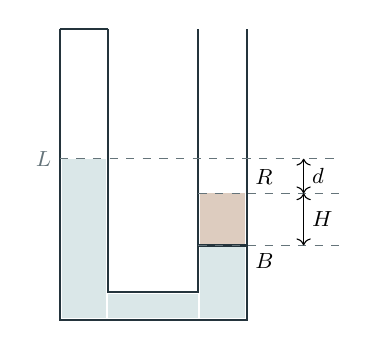
\begin{tikzpicture}[scale=.88,transform shape]
\draw[object](0,4.2)--(0,0)--(2.7,0)--(2.7,4.2);
\draw[object](.7,4.2)--(.7,.4)--(2,.4)--(2,4.2);\draw[object](0,4.2)--(.7,4.2);\fill[accent!16](.03,.03)rectangle(.67,2.325);\fill[accent!16](2.03,.03)rectangle(2.67,1.075);\fill[accent!16](.7,.03)rectangle(2,.37);\fill[warm!32](2.02,1.075)rectangle(2.68,1.825);\draw[object,line width=1pt](2,1.075)--(2.7,1.075);\draw[guide](0,2.325)node[left]{$L$}--(4.06,2.325);\draw[guide](2,1.825)--(4.06,1.825);\draw[guide](2,1.075)--(4.06,1.075);\node[above right]at(2.7,1.825){$R$};\node[below right]at(2.7,1.075){$B$};\draw[<->](3.52,1.825)--(3.52,2.325)node[midway,right]{$d$};\draw[<->](3.52,1.075)--(3.52,1.825)node[midway,right]{$H$};
\end{tikzpicture}
\figcaption{变图 热1.4V5\quad 汞上表面降低后，水的上行路径长为 $H+d$}
\end{minipage}\end{center}
\item 固定几何 $h_1,h_2,H$，因此 $L_f$ 与 $\sigma$ 无关。通过静压与等温式得到
\[
\frac{\partial p_0}{\partial\sigma}
=\rho_wg\frac{HL_f}{h_1-L_f}>0
\]
（$h_1>L_f$）。变图热1.4V6中，同一几何状态对应的大气压在 $\sigma=13.6$ 处为约195.21厘米水柱；每增加一个密度比单位，水柱高度增加 $HL_f/(h_1-L_f)\simeq18.214$ 厘米。若大气压固定，则提高密度后应联立新的静压与等温关系求位移。
\begin{center}\begin{minipage}{.98\linewidth}\centering
\begin{tikzpicture}[scale=.88,transform shape]
\draw[axis](0,0)--(6.1,0)node[right]{$\sigma$};\draw[axis](0,0)--(0,3.45)node[above]{$p_0/(\rho_wg)$};\draw[traj](1,0)--(5.64,2.535);\draw[guide](4.2153,0)node[below]{13.6}--(4.2153,1.756929)--(0,1.756929)node[left]{195.21 cm};\node[below]at(1,0){2.882};\fill(4.2153,1.756929)circle(1.5pt);
\end{tikzpicture}
\figcaption{变图 热1.4V6\quad 大气压水柱高度随上液密度比线性增大}
\end{minipage}\end{center}
\item 把水换成密度 $\rho'$ 的液体。若上液也按相同倍数改变密度，保持 $\rho_{\rm Hg}/\rho'=13.6$，静压各项都按同一倍数改变，所以同一几何所需的 $p_0$ 正比于 $\rho'$。若汞密度保持，则
\[
p_0=g\frac{\rho_{\rm Hg}HL_f-\rho'(HL_f+\Delta h_1)}{h_1-L_f}.
\]
本题 $\Delta>0$、$h_1>L_f$，上式对 $\rho'$ 的斜率为负。变图热1.4V7的两条直线在 $\rho'=\rho_w$ 处相交；归一化压强 $p_0/p_{0*}$ 的分母取这一组合所得大气压。相交点两种保持条件都回到水与水银的组合。
\begin{center}\begin{minipage}{.98\linewidth}\centering
\begin{tikzpicture}[scale=.88,transform shape]
\draw[axis](0,0)--(5.45,0)node[right]{$\rho^{\prime}/\rho_w$};\draw[axis](0,0)--(0,3.99)node[above]{$p_0/p_{0*}$};\draw[traj](.82,.656)--(4.6,3.68);\draw[warm,thick](.82,2.361449)--(4.60,1.548189);\draw[guide](2.5,0)node[below]{1}--(2.5,2)--(0,2)node[left]{1};\fill(2.5,2)circle(1.5pt);\node[right]at(4.6,3.68){定密度比};\node[right]at(4.6,1.548189){定上液密度};
\end{tikzpicture}
\figcaption{变图 热1.4V7\quad 两种保持条件给出方向相反的压强变化}
\end{minipage}\end{center}
\end{enumerate}

\Needspace{18\baselineskip}

\pdfbookmark[2]{第 5 题 玻璃管倒置插入水银槽的双气柱变化}{q5}

\section*{第 5 题\quad 玻璃管倒置插入水银槽的双气柱变化}

均匀直玻璃管一端A封闭、另一端B开口，中间有长$60\,\mathrm{mm}$的水银柱。水平放置时，A、B两侧空气柱均长$140\,\mathrm{mm}$。将管轻轻转为开口向下，再竖直插入水银槽；平衡后A端空气柱长$133\,\mathrm{mm}$。大气压强为$760\,\mathrm{mmHg}$，温度不变。求槽中水银进入管中的高度$H$，即从管口到管内槽水银面的距离。

\begin{center}\begin{minipage}{0.96\linewidth}\centering
\begin{tikzpicture}[x=1cm,y=1cm]
\draw[object] (0,0)--(0,.9)--(6.8,.9);\draw[object] (0,0)--(6.8,0);
\fill[warm!35] (2.8,0) rectangle(4,.9);
\draw[object] (2.8,0)--(2.8,.9);\draw[object] (4,0)--(4,.9);
\node at (1.4,.45) {A：140 mm};\node at (3.4,.45) {60 mm};\node at (5.4,.45) {B：140 mm};
\node[above] at (6.8,1) {开口};
\end{tikzpicture}\figcaption{图 热1.5　水平管中的两段气体均与760 mmHg相平衡。}\end{minipage}\end{center}

\Needspace{5\baselineskip}

\pdfbookmark[3]{题型定位}{q5-h0}

\subsection*{题型定位}

水平、倒置和插槽三阶段的双气柱问题。按两份气体各自封闭的时刻选等温关系的起点，再从管长和压差求入汞高及浸深。

\Needspace{5\baselineskip}

\pdfbookmark[3]{知识点}{q5-h1}

\subsection*{知识点}

等温气体只有在气量固定时才有 $pV$ 恒定。竖直汞柱上下两端相差 $\rho_{\rm Hg}gh$。装入槽中的管内汞与槽汞连通，内外自由液面的高差由槽上大气压和B气压共同确定。

\Needspace{5\baselineskip}

\pdfbookmark[3]{物理图像}{q5-h2}

\subsection*{物理图像}

图热1.5中水平汞柱两侧等压。解图热1.5A左侧倒置后，A从140毫米伸长到152毫米，B仍与大气相通，缩短到128毫米。右侧槽汞封住B，中间60毫米汞柱保持体积，上下两气柱各自缩短，进汞段补足管长。

\Needspace{5\baselineskip}

\pdfbookmark[3]{解题入口}{q5-h3}

\subsection*{解题入口}

用 $p_A'=760-60$ 和 $p_A'L_A'=760\times140$ 求出左图的A气长，从总管长推出B气长。右图由A末长求 $p_A''$，再由汞高求 $p_B''$，以B封口时的128毫米起算求B末长。

\Needspace{5\baselineskip}

\pdfbookmark[3]{标准解法}{q5-h4}

\subsection*{标准解法}

\textbf{阶段一：水平转为开口向下。}水银柱长度固定60 mm。B通大气，$p_B'=760\,\mathrm{mmHg}$；A在水银上方，故
\[p_A'=760-60=700\,\mathrm{mmHg}.\]
A气体一直封闭，等温关系给出
\[L_A'=\frac{760\times140}{700}=152\,\mathrm{mm}.\]
总管长$140+60+140=340\,\mathrm{mm}$，因此
\[L_B'=340-60-152=128\,\mathrm{mm}.\]
B从140 mm变为128 mm时压强仍为760 mmHg，有相当于12 mm初始气柱的气体外泄。插槽后的定量过程从倒置后的128毫米起算。
\begin{center}\begin{minipage}{0.96\linewidth}\centering
\begin{tikzpicture}[x=1cm,y=1cm]
\fill[accent!8] (0,0) rectangle(2,1.28);
\fill[warm!35] (0,1.28) rectangle(2,1.88);
\fill[accent!8] (0,1.88) rectangle(2,3.4);
\draw[object] (0,0)--(0,3.4)--(2,3.4)--(2,0);
\node[align=center,font=\footnotesize] at (1,.64) {B\\128 mm\\760 mmHg};
\node[font=\footnotesize] at (1,1.58) {汞：60 mm};
\node[align=center,font=\footnotesize] at (1,2.64) {A\\152 mm\\700 mmHg};
\node[below] at (1,-.3) {倒置，B开口};
\draw[motion] (2.4,.6)--(2.4,-.15) node[right,midway] {外泄};
\fill[warm!18] (4.2,-.15) rectangle(8.2,1.33883721);
\draw[object] (4.2,1.45)--(4.2,-.15)--(8.2,-.15)--(8.2,1.45);
\fill[white] (5,0) rectangle(7,3.4);
\fill[warm!35] (5,0) rectangle(7,.33883721);
\fill[accent!8] (5,.33883721) rectangle(7,1.47);
\fill[warm!35] (5,1.47) rectangle(7,2.07);
\fill[accent!8] (5,2.07) rectangle(7,3.4);
\draw[object] (5,0)--(5,3.4)--(7,3.4)--(7,0);
\draw[guide] (4.2,1.33883721)--(5,1.33883721);
\draw[guide] (7,1.33883721)--(8.2,1.33883721);
\node[align=center,font=\footnotesize] at (6,.91) {B\\113.116 mm\\860 mmHg};
\node[font=\footnotesize] at (6,1.77) {汞：60 mm};
\node[align=center,font=\footnotesize] at (6,2.735) {A\\133 mm\\800 mmHg};
\node[below] at (6,-.3) {插槽后};
\node[above left,font=\footnotesize] at (4.6,1.42) {$p_0=760$ mmHg};
\draw[<->] (7.4,0)--(7.4,.33883721) node[right,midway] {$H$};
\draw[<->] (7.4,.33883721)--(7.4,1.33883721) node[right,midway,font=\footnotesize] {100 mm};
\draw[<->] (9.2,0)--(9.2,1.33883721) node[right,midway] {$d$};
\end{tikzpicture}\figcaption{解图 热1.5A　管内槽汞面比槽外液面低100 mm。$H$ 从管口量到管内槽汞面，$d$ 从管口量到槽外液面。}\end{minipage}\end{center}
\textbf{阶段二：插入水银槽，B也被封闭。}解图热1.5A右侧给定$L_A''=133\,\mathrm{mm}$，于是
\[p_A''=\frac{760\times140}{133}=800\,\mathrm{mmHg},\qquad
p_B''=p_A''+60=860\,\mathrm{mmHg}.\]
解图热1.5A中，上下两份气体各沿自己的等温曲线变化。A的守恒量始终是$760\times140$，B只有在管口被槽水银封住之后才有固定的$760\times128$。两组长度的先后关系可列为
\[\begin{array}{c|cc}
&A&B\\\hline
\text{最初水平}&140&140\\
\text{倒置且B开口}&152&128\\
\text{插槽后}&133&L_B''
\end{array}\qquad(\text{长度单位：mm}).\]
最后一行中，60毫米水银柱隔开两份气体，并使下侧的压强比上侧高60毫米汞柱。

对\emph{倒置后留下的}B气体列式：
\[760\times128=860L_B'',\qquad L_B''=113.116\,\mathrm{mm}.\]
管内空间还包括原有60 mm水银柱和槽中进入的水银$H$，故
\result{H=340-60-133-113.116=33.884\,\mathrm{mm}\approx34\,\mathrm{mm}.}
右图中 $p_B''>p_0$，管内槽水银面低于槽外液面；两面相差$860-760=100\,\mathrm{mm}$。所以管口浸入深度为$H+100=133.884\,\mathrm{mm}$。
\subsubsection*{气体外泄量与插槽后各段高度}
图热1.5中原有水银柱隔开A、B两段气体。倒置时A始终封闭，
B仍与大气相通，所以水平状态到倒置状态只有A可直接用$pL$守恒。
若管截面积为$S$，倒置时B外泄的摩尔数及其占初量的比例为
\[
\Delta n_B=\frac{p_0S(140-128)}{RT},\qquad
\frac{\Delta n_B}{n_{B,0}}=\frac{12}{140}=\frac3{35}.
\]
这里的12毫米是将外泄气量按初温、初压折算成的等效气柱长度。
A和B始终由原有汞柱隔离，B外泄也不改变A的气量。

解图热1.5A的右管口与槽水银接触后，B的气量固定为
$p_0S\times128/(RT)$；右侧气柱下方新进入的汞与槽内汞连通，
上方60毫米汞柱则仍与它隔着B气体。应分别比较这两段汞：
上汞柱给$p_B''-p_A''=60\,\mathrm{mmHg}$，
下段槽汞给$p_B''-p_0=\rho_{\rm Hg}g(d-H)$。
用毫米汞柱为压强数值单位，后一式为
\[
d-H=p_B''-760=100\,\mathrm{mm},\qquad
d=133.883721\,\mathrm{mm}.
\]
图中$H$从管口量到管内槽汞面，$d-H$是内外自由液面的高差，
$d$才是管口在槽面下的深度。三个高度有各自的端点，解图热1.5A右侧的三个标注分别从这些端点量起。

插槽过程进入的汞正好填满两气柱缩短所腾出的空间：
\[
H=(152-133)+(128-113.116279)
=19+14.883721=33.883721\,\mathrm{mm}.
\]
左式以倒置并刚封住B的状态为起点；
若以最初水平状态计算，则A只净缩短7毫米，而B长度的变化还包含12毫米的外泄，
先从B的总缩短量扣掉外泄对应的12毫米，所得才是插槽阶段的缩短量。

固定这两份已封闭的气体，设末态A压强的数值为$q$，仍用mmHg。
两气长、管内入汞高度及口的浸入深度可写为
\[
L_A(q)=\frac{760\times140}{q},\qquad
L_B(q)=\frac{760\times128}{q+60},\qquad
H(q)=280-L_A(q)-L_B(q),
\]
\[
d(q)=H(q)+q+60-760.
\]
$q=700$对应$H=d=0$的刚封口状态，之后$d$随$q$严格增大，
因为
\[
\frac{\dd d}{\dd q}
=1+\frac{760\times140}{q^2}
+\frac{760\times128}{(q+60)^2}>0.
\]
这一关系可用于“给定浸入深度，反求两气柱”的变式，并保证在气柱均保持正长的区间内解唯一。
本题$q=800$代回同时得到$L_A=133$毫米和已经求得的$H,d$。


\Needspace{5\baselineskip}

\pdfbookmark[3]{关键洞察}{q5-h5}

\subsection*{关键洞察}

从水平到倒置，B开放时变化的是气量；从倒置到插槽，B定量时变化的是气压。插槽后的两个气柱各缩短19及14.883721毫米，两段缩短量的和就是入汞高。槽内外液面差100毫米由B压强另行给出。

\Needspace{5\baselineskip}

\pdfbookmark[3]{易错点}{q5-h6}

\subsection*{易错点}

解图热1.5A左图中A在汞柱上方，$p_A'=p_0-60$；右图中B在中间汞柱下方，$p_B''=p_A''+60$。B从开口时的128毫米进入定量过程。将进汞高 $H$、液面差 $d-H$ 和管口浸深 $d$ 各写在相应两个端点之间。

变参数时，倒置后需保持中间汞柱完整、B气柱仍有正长度，见变图热1.5V1。

\Needspace{5\baselineskip}

\pdfbookmark[3]{课堂讲解建议}{q5-h7}

\subsection*{课堂讲解建议}

让学生按解图热1.5A左、右图分别给A、B注明压强、长度与通断状态。先算B外泄量为初量的 $3/35$，再在图中指出连接800与860毫米汞柱的中间汞柱，以及连接860与760毫米汞柱的槽汞。

遮住右图的高度标注，请学生从端点重新量出 $H,d-H,d$。给定另一个浸深时，用变图热1.5V4上斜率为正的曲线反读 $q$，然后从 $q$ 恢复两气柱长度。


\Needspace{5\baselineskip}

\pdfbookmark[3]{变式训练}{q5-h8}

\subsection*{变式训练}

\begin{enumerate}
\item 设初始A、B气柱长为 $a,b$，中间汞高为 $h$，大气压用同单位的汞柱高度 $P$ 表示。倒置后B仍通大气，故 $p_A'=P-h$，$L_A'=Pa/(P-h)$，$L_B'=a+b-L_A'$。$L_B'>0$ 等价于
\[
h<\frac{Pb}{a+b},
\]
此时也有 $P>h$。在变图热1.5V1的交点处，B气柱缩为零，汞下端抵达管口；再增大 $h$ 会有汞流出，后续应按留在管内的汞量求压强。图取 $P=760,a=b=140$，交点 $h=380\,\mathrm{mm}$。
\begin{center}\begin{minipage}{.98\linewidth}\centering
\begin{tikzpicture}[scale=.88,transform shape]
\draw[axis](0,0)--(4.48,0)node[right]{$h/\mathrm{mm}$};\draw[axis](0,0)--(0,3.45)node[above]{$L_B^\prime/\mathrm{mm}$};\draw[traj,domain=0:3.8,samples=77]plot(\x,{(280-10640/(76-10*\x))/50});\node[left]at(0,2.8){140};\filldraw[fill=white,draw=accent](3.8,0)circle(1.5pt)node[below]{380};
\end{tikzpicture}
\figcaption{变图 热1.5V1\quad 开口朝下时，B气柱长随初汞高增加而缩短}
\end{minipage}\end{center}
\item 开口改为朝上，变图热1.5V2右管的A位于汞柱下面。竖直压强为 $P+h$，所以 $L_A'=Pa/(P+h)<a$，$L_B'=a+b-L_A'>b$。B保持大气压，吸入相当于 $a-L_A'$ 气柱长的空气。左管开口朝下时A在汞柱上方，B外泄。若随后让朝上的管口接触槽汞，插入方式给出哪些气体被封住以及槽液面所在位置，应按该方式另列静压关系。
\begin{center}\begin{minipage}{.98\linewidth}\centering
\begin{tikzpicture}[scale=.88,transform shape]
\begin{scope}[xshift=0cm]
\fill[accent!11](0,0)rectangle(1.23,1.28);\fill[warm!33](0,1.28)rectangle(1.23,1.88);
\fill[accent!11](0,1.88)rectangle(1.23,3.4);\draw[object](0,0)--(0,3.4)--(1.23,3.4)--(1.23,0);
\node at(.615,0.64){B};\node at(.615,2.6399999999999997){A};
\end{scope}\begin{scope}[xshift=3.35cm]
\fill[accent!11](0,0)rectangle(1.23,1.2975609756097561);\fill[warm!33](0,1.2975609756097561)rectangle(1.23,1.897560975609756);
\fill[accent!11](0,1.897560975609756)rectangle(1.23,3.3999999999999995);\draw[object](0,3.3999999999999995)--(0,0)--(1.23,0)--(1.23,3.3999999999999995);
\node at(.615,0.6487804878048781){A};\node at(.615,2.6487804878048777){B};
\end{scope}\draw[motion](1.54,.59)--(1.54,-.31)node[right]{排气};\draw[motion](4.92,3.94)--(4.92,3.30)node[right]{进气};\node at(.615,3.85){开口朝下};\node at(3.965,-.4){开口朝上};
\end{tikzpicture}
\figcaption{变图 热1.5V2\quad 开口取向改变后，B气柱的进、排气方向交换}
\end{minipage}\end{center}
\item 两初气长改为 $a,b$ 且 $a\ne b$，继续开口朝下。满足变式1的气长条件时，A伸长
\[
\Delta L=L_A'-a=\frac{ah}{P-h},\qquad
\frac{\Delta n_B}{n_{B,0}}=\frac{\Delta L}{b}.
\]
变图热1.5V3中，B体积少去与A伸长同样的一段。封口后，B的 $pL$ 常量为 $P[a+b-Pa/(P-h)]$。例如取 $a=100,b=180,P=760,h=60$，B缩短 $8.571$ 毫米，余下 $171.429$ 毫米。
\begin{center}\begin{minipage}{.98\linewidth}\centering
\begin{tikzpicture}[scale=.88,transform shape]
\fill[accent!12](0,0)rectangle(2,.5);\fill[warm!32](2,0)rectangle(3.2,.5);\fill[accent!25](3.2,0)rectangle(6.8,.5);\fill[accent!12](0,1.04)rectangle(2.17143,1.54);\fill[warm!32](2.17143,1.04)rectangle(3.37143,1.54);\fill[accent!25](3.37143,1.04)rectangle(6.8,1.54);\foreach \y in {.25,1.29}{\node at(1,\y){A};\node at(5,\y){B};}\draw[guide](2,-.08)--(2,1.64);\draw[guide](2.17143,.53)--(2.17143,1.64);\draw[<->](2,1.76)--(2.17143,1.76);\node[above]at(2.086,1.82){$\Delta L$};\node[right]at(6.88,.25){水平};\node[right]at(6.88,1.29){倒置};
\end{tikzpicture}
\figcaption{变图 热1.5V3\quad 同一标尺上，A伸长等于B缩短}
\end{minipage}\end{center}
\item 给定管口浸深 $d$。令A压强为 $q$，$L_A=Pa/q$，$L_B=PL_B'/(q+h)$，所以 $H=a+b-L_A-L_B$。槽汞的压强关系给 $d=H+q+h-P$，求导得
\[
\frac{\dd d}{\dd q}=1+\frac{Pa}{q^2}+\frac{PL_B'}{(q+h)^2}>0.
\]
变图热1.5V4从 $q=P-h$ 的刚封口状态出发，浸深沿曲线严格增加。每个曲线覆盖的浸深给出唯一 $q$，由此恢复两段气长和 $H$。例如 $d=133.883721$ 毫米对应 $q=800$ 毫米汞柱。
\begin{center}\begin{minipage}{.98\linewidth}\centering
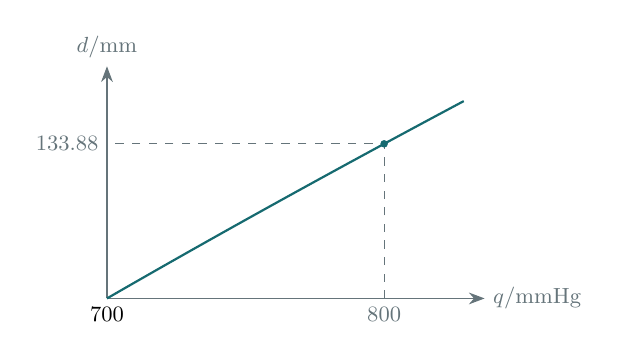
\begin{tikzpicture}[scale=.88,transform shape]
\draw[axis](0,0)--(5.45,0)node[right]{$q/\mathrm{mmHg}$};\draw[axis](0,0)--(0,3.35)node[above]{$d/\mathrm{mm}$};\draw[traj,domain=0:5.15,samples=77]plot(\x,{4.6666667-1773.3333/(700+25*\x)-1621.3333/(760+25*\x)+25*\x/60});\node[below]at(0,0){700};\draw[guide](4,0)node[below]{800}--(4,2.231395)--(0,2.231395)node[left]{133.88};\fill[accent](4,2.231395)circle(1.55pt);
\end{tikzpicture}
\figcaption{变图 热1.5V4\quad 浸深沿单调曲线给出唯一的A压强}
\end{minipage}\end{center}
\item 若形式代入给 $p_A'=P-h\le0$，在 $n_A>0$ 且正体积有限的气体状态中，$p_A'=n_ART/V_A$ 始终为正。变图热1.5V5取 $a=b$，当 $h=P/2$ 时，B已缩至零。更大的汞高使倒置时的汞流出，固定初汞高的关系只覆盖图中实线段。此时应重新确定管中实际余汞量及气体通断情况，再写新的静压与状态式。
\begin{center}\begin{minipage}{.98\linewidth}\centering
\begin{tikzpicture}[scale=.88,transform shape]
\draw[axis](0,0)--(5.28,0)node[right]{$h/P$};\draw[axis](0,0)--(0,3.1)node[above]{$p_A^\prime/P$};\draw[traj](0,2.55)--(2.2,1.275);\draw[guide](2.2,1.275)--(4.4,0);\draw[guide](2.2,0)node[below]{$1/2$}--(2.2,1.275);\node[below]at(4.4,0){1};\node[left]at(0,2.55){1};\node[above]at(1.14,2.20){汞完整留管};\node[above right]at(2.57,1.15){形式延长};
\end{tikzpicture}
\figcaption{变图 热1.5V5\quad 在形式压力降至零前，B气柱已先缩至零}
\end{minipage}\end{center}
\item 使末态A气柱比133毫米更短，两气体仍封闭。随着 $L_A$ 减小，$p_A=760\times140/L_A$ 增大，$p_B=p_A+60$ 同步增大，$L_B=760\times128/p_B$ 减小。于是 $H=280-L_A-L_B$ 和外液面差 $p_B-760$ 都增大。变图热1.5V6取 $q=800,880$ 毫米汞柱，前者两段分别为33.884、100毫米，后者为55.602、180毫米。两段总和就是管口浸深 $d$。
\begin{center}\begin{minipage}{.98\linewidth}\centering
\begin{tikzpicture}[scale=.88,transform shape]
\draw[axis](0,0)--(4.92,0)node[right]{$q/\mathrm{mmHg}$};\draw[axis](0,0)--(0,3.86)node[above]{高度$/\mathrm{mm}$};\fill[accent!36](.85,0)rectangle(1.82,.508256);\fill[warm!37](.85,.508256)rectangle(1.82,2.008256);\fill[accent!36](2.89,0)rectangle(3.86,0.834023);\fill[warm!37](2.89,0.834023)rectangle(3.86,3.534023);\node at(1.335,.25){$H$};\node at(3.375,.40){$H$};\node at(1.335,1.22){$d-H$};\node at(3.375,2.18){$d-H$};\node[below]at(1.335,0){800};\node[below]at(3.375,0){880};
\end{tikzpicture}
\figcaption{变图 热1.5V6\quad A被压缩时，进汞高与内外液面差均增大}
\end{minipage}\end{center}
\item 保持 $P,a,b$，增大初汞高。汞完整留在倒置管内的区间为 $h<Pb/(a+b)$，在这段内
\[
\Delta L=\frac{ah}{P-h},\qquad
\frac{\dd\Delta L}{\dd h}=\frac{aP}{(P-h)^2}>0 .
\]
变图热1.5V7取 $a=b=140\,\mathrm{mm}$，外泄的等效长度到 $h=380$ 毫米时趋近 $b$。到这个位置时，B原来所含气体恰被全部挤出。
\begin{center}\begin{minipage}{.98\linewidth}\centering
\begin{tikzpicture}[scale=.88,transform shape]
\draw[axis](0,0)--(4.53,0)node[right]{$h/\mathrm{mm}$};\draw[axis](0,0)--(0,3.65)node[above]{$\Delta L/\mathrm{mm}$};\draw[traj,domain=0:3.8,samples=77]plot(\x,{2.8*\x/(7.6-\x)});\draw[guide](3.8,0)node[below]{380}--(3.8,2.8)--(0,2.8)node[left]{140};\fill[accent](3.8,2.8)circle(1.5pt);
\end{tikzpicture}
\figcaption{变图 热1.5V7\quad B的外泄量沿曲线增至初始气量}
\end{minipage}\end{center}
\end{enumerate}

\clearpage

\pdfbookmark[2]{第 6 题 升温推动水银柱外溢的分阶段判断}{q6}

\section*{第 6 题\quad 升温推动水银柱外溢的分阶段判断}

均匀玻璃管长$96\,\mathrm{cm}$，下端封闭，上端开口。管内有长$20\,\mathrm{cm}$的水银柱；$27^\circ\mathrm C$时，其下封闭空气柱长$60\,\mathrm{cm}$。外界压强为$76\,\mathrm{cmHg}$。缓慢升温，求导致水银全部溢出的临界温度。忽略管和水银的热膨胀，空气视为理想气体。须区分水银刚到管口、稳定部分外溢和失稳后迅速排出的阶段。

\begin{center}\begin{minipage}{0.96\linewidth}\centering
\begin{tikzpicture}[x=1cm,y=1cm]\fill[accent!8] (0, 0) rectangle (1.7,2.4);
\node[align=center,font=\footnotesize] at (0.85,1.2) {空气\\60 cm};
\fill[warm!35] (0, 2.4) rectangle (1.7,3.2);
\node[align=center,font=\footnotesize] at (0.85,2.8) {汞\\20 cm};
\node[align=center,font=\footnotesize] at (0.85,3.52) {空隙\\16 cm};
\draw[object] (0,0)--(0,3.8400000000000003);\draw[object] (1.7,0)--(1.7,3.8400000000000003);
\draw[object] (0,0)--(1.7,0);
\node[align=center] at (0.85,-.55) {27℃};
\node at (4,3.6) {$p_a=76\,\mathrm{cmHg}$};\draw[motion] (3,.7)--(3,2) node[right,midway]{升温};
\end{tikzpicture}\figcaption{图 热1.6　水银尚未到管口，完整水银柱使封闭空气压强保持96 cmHg。}\end{minipage}\end{center}

\Needspace{5\baselineskip}

\pdfbookmark[3]{题型定位}{q6-h0}

\subsection*{题型定位}

封闭气体加热推动汞柱的分段过程。到口前求等压膨胀，到口后求有限汞长的平衡曲线及流失开始自行加剧的临界点。

\Needspace{5\baselineskip}

\pdfbookmark[3]{知识点}{q6-h1}

\subsection*{知识点}

固定汞长时气压为 $P+h$。部分外溢后，汞长 $x$ 同时给出气长 $L-x$ 和气压 $P+x$。定量理想气体满足 $pV/T$ 恒定；温度方程的两根分别给出两个汞长，实际过程从到口的 $x=h$ 连续出发。

\Needspace{5\baselineskip}

\pdfbookmark[3]{物理图像}{q6-h2}

\subsection*{物理图像}

图热1.6初始开口空隙为16厘米。解图热1.6A左图中，气柱伸至76厘米时汞到口；右图表明每流出一段汞就腾出同样长度给空气。沿解图热1.6B的箭头，剩余汞长由20减至10厘米，平衡温度同时升高。

\Needspace{5\baselineskip}

\pdfbookmark[3]{解题入口}{q6-h3}

\subsection*{解题入口}

用 $T_0=300.15\,\mathrm K$ 和初态 $p_iL_0/T_0$ 固定气量。到口前用等压比例求 $T_1$，到口后把 $(76+x)(96-x)$ 配成 $7396-(x-10)^2$。对少量外溢产生的 $\delta x<0$，由气压与负载压差 $D$ 判断能否停止。

\Needspace{5\baselineskip}

\pdfbookmark[3]{标准解法}{q6-h4}

\subsection*{标准解法}

\textbf{完整水银柱阶段。}初温$T_0=300.15\,\mathrm K$，初压$p_i=76+20=96\,\mathrm{cmHg}$。完整汞柱上方尚有16 cm空隙，加热时气体等压膨胀。汞柱上端刚到管口时气长$96-20=76\,\mathrm{cm}$，因此
\[\frac{96\times60}{T_0}=\frac{96\times76}{T_1},\qquad
T_1=T_0\frac{76}{60}=380.19\,\mathrm K.\]
\begin{center}\begin{minipage}{0.96\linewidth}\centering
\begin{tikzpicture}[x=1cm,y=1cm]\fill[accent!8] (0, 0) rectangle (1.6,3.04);
\node[align=center,font=\footnotesize] at (0.8,1.52) {气：76 cm};
\fill[warm!35] (0, 3.04) rectangle (1.6,3.84);
\node[align=center,font=\footnotesize] at (0.8,3.44) {汞：20 cm};
\draw[object] (0,0)--(0,3.84);\draw[object] (1.6,0)--(1.6,3.84);
\draw[object] (0,0)--(1.6,0);
\node[align=center] at (0.8,-.55) {刚到管口};
\fill[accent!8] (3.8, 0) rectangle (5.4,3.24);
\node[align=center,font=\footnotesize] at (4.6,1.62) {气：$96-x$};
\fill[warm!35] (3.8, 3.24) rectangle (5.4,3.84);
\node[align=center,font=\footnotesize] at (4.6,3.54) {汞：$x$};
\draw[object] (3.8,0)--(3.8,3.84);\draw[object] (5.4,0)--(5.4,3.84);
\draw[object] (3.8,0)--(5.4,0);
\node[align=center] at (4.6,-.55) {部分外溢};
\draw[motion] (5.6,3.7)--(6.5,3.7) node[right]{溢出};
\end{tikzpicture}\figcaption{解图 热1.6A　右图取余汞长 $x=15\,\mathrm{cm}$ 的部分外溢状态。气柱同时变长，水银的附加压强减小。}\end{minipage}\end{center}
\textbf{部分外溢阶段。}解图热1.6A右侧设剩余汞长$x$，则气长$96-x$、气压$76+x$。封闭空气摩尔数仍不变，
\[\frac{96\times60}{T_0}=\frac{(76+x)(96-x)}{T}.\]
将乘积展开并配方：
\[(76+x)(96-x)=7296+20x-x^2=7396-(x-10)^2,\]
于是
\[T(x)=\frac{T_0}{5760}\bigl[7396-(x-10)^2\bigr],\quad
x_\pm=10\pm\sqrt{7396-\frac{5760T}{T_0}}.\]
实根条件为$T\le T_c$，其中
\result{T_c=\frac{7396}{5760}T_0=385.40\,\mathrm K
\approx112.25^\circ\mathrm C.}
若用$T_0\approx300\,\mathrm K$，则$T_c\approx385.21\,\mathrm K$，通常粗略记为385 K。
\begin{center}\begin{minipage}{0.96\linewidth}\centering
\begin{tikzpicture}[x=1cm,y=1cm]
\draw[axis] (0,0)--(5.5,0) node[right] {$x/\mathrm{cm}$};
\draw[axis] (0,0)--(0,3.1) node[above] {$(T-T_1)/(T_c-T_1)$};
\draw[traj,domain=0:5,samples=90] plot (\x,{2.4*(1-pow((4*\x-10)/10,2))});
\draw[guide] (2.5,0) node[below]{10}--(2.5,2.4)--(0,2.4) node[left]{1};
\node[below left] at (0,0) {0};\node[below] at (5,0) {20};
\fill[accent] (5,0) circle(1.5pt);\fill[accent] (2.5,2.4) circle(1.5pt);
\draw[motion,domain=4.5:3.7,samples=25] plot (\x,{2.4*(1-pow((4*\x-10)/10,2))});
\node[align=center,font=\footnotesize] at (4.3,2.9) {加热所循\\$x_+$支};
\node at (1.15,1.05) {$x_-$支};
\end{tikzpicture}\figcaption{解图 热1.6B　纵轴为到口后的归一化温升；加热过程从20 cm沿右支到10 cm临界点。}\end{minipage}\end{center}
\textbf{从到口态选择加热分支。}在到口温度 $T_1$，解图热1.6B 的两根为 $x_+=20$、$x_-=0$。已知到口时管内仍有20厘米汞，因此从 $x_+=20$ 出发，随加热沿右支减到10厘米。

定温时，少量外溢后的压差决定流失能否停止。固定温度下，气体在某个$x$产生的压强（单位cmHg）为$P_g=5760T/[T_0(96-x)]$；需平衡的外压为$P_e=76+x$。令$D=P_g-P_e$，在平衡点
\[\frac{\dd D}{\dd x}=\frac{76+x}{96-x}-1
=\frac{2x-20}{96-x}.\]
少量水银溢出使$x$减小。$x>10$时$D$随之变负，气压不足以继续推出水银，因而能停在部分外溢状态；$x<10$时$D$变正，进一步推动外溢。到$x=10$时两根合并，再升温就没有平衡解。

所以全部溢出由超过$T_c$后的失稳触发，所求是这一临界温度。在 $T=T_c$ 的无扰动状态下，尚有10厘米水银留在管内。在缓慢加热、忽略快速排出中的温变和耗散细节的模型中，稍超过385.4 K，余汞迅速排出。
\subsubsection*{判别式、连续分支与临界点的单向扰动}
图热1.6中封闭气体的初始状态满足
\[
\frac{p_iL_0}{T_0}=\frac{96\times60}{300.15},
\]
这是两个阶段共同保留的气量条件；初始封闭气体在汞柱下方，其气长是60厘米；16厘米的开口空隙在汞柱上方。
汞尚未到口时，压强固定为$96\,\mathrm{cmHg}$；
汞到口后，剩余长度$x$同时决定气压$76+x$和气长$96-x$，相应的两个量沿同一平衡曲线变化。

把部分外溢状态的方程整理为二次式：
\[
x^2-20x+\frac{5760T}{T_0}-7296=0,\qquad
\Delta=4\left(7396-\frac{5760T}{T_0}\right).
\]
除$\Delta\ge0$外，实际根还须满足$0\le x\le20$，并与到口状态$x=20$连续相接。
在$T=T_1$，两根恰为20与0；加热初期应取从20厘米开始的$x_+$。
当温度从$T_1$增至$T_c$，$x_+$从20厘米减至10厘米，
左支 $x_-$ 从0增至10厘米，随加热反而要求管内汞增多。

解图热1.6B的纵轴用$(T-T_1)/(T_c-T_1)$归一化，
两个端点$x=0,20$都在零线，峰值$x=10$在1线上。
因此沿右支加热时，图上是向左、向上运动；临界点仍有半根汞柱留在管内。
临界温度与到口温度相差
\[
T_c-T_1=\frac{100}{5760}T_0
=5.2109375\,\mathrm K,
\]
这5.21开尔文对应刚到口与失稳之间的部分外溢阶段。

这里的“稳定”指少量汞已流出后能否停止继续外溢；
负的压差会使管内余汞退回口内，流出的汞留在管外。
固定$T$时，气压与所需外压之差可精确写成
\[
D(x;T)=\frac{5760T/T_0-(76+x)(96-x)}{96-x}.
\]
在平衡点$x_e>10$，微小外溢给$\delta x<0$，
$D\simeq[(2x_e-20)/(96-x_e)]\delta x<0$，气压不足以继续推出汞，
汞上面退到口内后，外溢可在该温度下停止。
在$x_e<10$处，相同外溢扰动给$D>0$，推动进一步流失。

恰在临界温度，一阶项消失，直接代入精确式得
\[
D(x;T_c)=\frac{(x-10)^2}{96-x}\ge0.
\]
无扰动时 $x=10$ 可保持瞬时平衡。若再流出少量汞，$x<10$ 时的正二阶压差继续推动外溢。
在温度保持或继续超过$T_c$的热学模型下，有限剩余汞已没有可持续的平衡终态。
排出阶段的温度和流速随时间变化；若要计算，需另列气体能量方程与液体运动方程。这里求的临界温度是定温平衡分支的终点。


\Needspace{5\baselineskip}

\pdfbookmark[3]{关键洞察}{q6-h5}

\subsection*{关键洞察}

实际加热支的来路在解图热1.6B的右端。右支上少量流失给负压差，余汞可以退入口内；左支上相同流失给正压差，气体继续推汞。顶点处一阶项消失，精确式的平方项仍在流失后产生正压差。超过临界温度，连右支的可续状态也消失。

\Needspace{5\baselineskip}

\pdfbookmark[3]{易错点}{q6-h6}

\subsection*{易错点}

在解图热1.6A换到右图时，同时更新 $P+x$ 和 $L-x$。先从20厘米的到口态接到右支，再用 $0\le x\le20$ 限定汞长。到口温度用 $T_1$，失稳温度用 $T_c$；计算从摄氏温度换为绝对温度后进行。

临界点的压差符号由 $(x-10)^2/(96-x)$ 给出，比较的是少量流失后的状态。

\Needspace{5\baselineskip}

\pdfbookmark[3]{课堂讲解建议}{q6-h7}

\subsection*{课堂讲解建议}

先让学生从图热1.6读出初始气长及开口空隙，画解图热1.6A左、右两状态。随后在解图热1.6B画一条位于 $T_1$ 与 $T_c$ 之间的水平线，请学生说明哪一根来自完整汞柱。

固定温度并从两支各取一点，把剩余汞长减去一小段，比较所需平衡气压和实际气压。再在顶点作同样操作，由精确压差读出二阶项，帮助学生区分无扰动的临界平衡与扰动后的快速排出。


\Needspace{5\baselineskip}

\pdfbookmark[3]{变式训练}{q6-h8}

\subsection*{变式训练}

\begin{enumerate}
\item 设 $L,h,l,P,T_0$ 分别为管长、初汞长、初气长、大气压所对应的汞高和初温，且 $l+h\le L$。完整汞柱到口时，气柱长为 $L-h$，所以 $T_1=T_0(L-h)/l$。后续按
\[
T(x)=\frac{T_0(P+x)(L-x)}{(P+h)l},\qquad 0\le x\le h .
\]
求导可知斜率与 $L-P-2x$ 同号。变图热1.6V1示出 $0<x_c=(L-P)/2<h$ 时的情形；加热使 $x$ 从 $h$ 减小并追踪到 $x_c$，这段曲线的斜率为负。若顶点位于允许区间外，则比较 $0,h$ 两端及它们的斜率。
\begin{center}\begin{minipage}{.98\linewidth}\centering
\begin{tikzpicture}[scale=.88,transform shape]
\draw[axis](0,0)--(5.95,0)node[right]{$x$};\draw[axis](0,-.23)--(0,3.36)node[above]{$T$};\draw[traj,domain=0:5.2,samples=75]plot(\x,{.88+2.1*(1-(\x/2.6-1)^2)});\draw[guide](2.6,0)node[below]{$x_c$}--(2.6,2.98);\draw[guide](5.2,0)node[below]{$h$}--(5.2,.88)--(0,.88)node[left]{$T_1$};\draw[motion,domain=4.7:3.4,samples=28]plot(\x,{.88+2.1*(1-(\x/2.6-1)^2)});\fill[accent](2.6,2.98)circle(1.6pt);\fill[accent](5.2,.88)circle(1.6pt);
\end{tikzpicture}
\figcaption{变图 热1.6V1\quad 允许区间内，升温分支从完整汞柱一端向顶点移动}
\end{minipage}\end{center}
\item 令 $x_c=(L-P)/2$。若 $0<x_c<h$，加热从 $x=h$ 到 $x=x_c$，临界温度为
\[
T_c=\frac{T_0(L+P)^2}{4(P+h)l}.
\]
若 $x_c\ge h$，到口时已在抛物线的递增段或顶点，再升温就没有连续可走的部分外溢支，触发温度为 $T_1$。若 $x_c\le0$，$x$ 递减时温度一直升高，沿平衡支排尽，端点温度为 $T_{\rm end}=T_0PL/[(P+h)l]$。变图热1.6V2取 $L=96\,\mathrm{cm},h=20\,\mathrm{cm}$，比较三个 $P$ 下各曲线相对到口态的变化。
\begin{center}\begin{minipage}{.98\linewidth}\centering
\begin{tikzpicture}[scale=.88,transform shape]
\draw[axis](0,0)--(5.88,0)node[right]{$x/\mathrm{cm}$};\draw[axis](0,-2.15)--(0,2.56)node[above]{$F(x)-F(h)$};\draw[traj,domain=0:5,samples=75]plot(\x,{(20-4*\x)*(4*\x)/200});\draw[traj,dotted,domain=0:5,samples=75]plot(\x,{(20-4*\x)*(20+4*\x)/200});\draw[guide,domain=0:5,samples=75]plot(\x,{-(20-4*\x)^2/200});\node[right]at(.55,2.25){$P=96$};\node[above]at(2.55,.51){$P=76$};\node[right]at(.55,-1.82){$P=56$};\node[below]at(5,0){20};\fill(5,0)circle(1.5pt);\node[above right]at(5,0){到口};
\end{tikzpicture}
\figcaption{变图 热1.6V2\quad 用 $F(x)=(P+x)(L-x)$ 比较外压改变后的允许分支}
\end{minipage}\end{center}
\item 若初汞长 $h$ 大于上方空隙 $g=L-l-h$，仍有 $g\ge0$。变图热1.6V3的右图中，整柱仅上移长度 $g$ 就到达管口，两态的汞长都为 $h$。等压关系给
\[
T_1-T_0=T_0\frac{g}{l}.
\]
例如本题 $h=20\,\mathrm{cm}$、$g=16\,\mathrm{cm}$，气柱从60伸至76厘米，温升为80.04开尔文。若 $g=0$，初态已到口，该阶段的温升为零。
\begin{center}\begin{minipage}{.98\linewidth}\centering
\begin{tikzpicture}[scale=.88,transform shape]
\begin{scope}[xshift=0cm]
\fill[accent!16](0,0)rectangle(1.1,2.4);\fill[warm!30](0,2.4)rectangle(1.1,3.2);
\draw[object](0,3.84)--(0,0)--(1.1,0)--(1.1,3.84);
\node at(.55,1.2){气};\node at(.55,2.8){汞};\node[below]at(.55,-.13){初态};
\end{scope}\begin{scope}[xshift=3.4cm]
\fill[accent!16](0,0)rectangle(1.1,3.04);\fill[warm!30](0,3.04)rectangle(1.1,3.84);
\draw[object](0,3.84)--(0,0)--(1.1,0)--(1.1,3.84);
\node at(.55,1.52){气};\node at(.55,3.44){汞};\node[below]at(.55,-.13){刚到口};
\end{scope}\draw[<->](1.33,3.2)--(1.33,3.84)node[midway,right]{$g$};\draw[guide](1.1,3.2)--(3.34,3.2);\draw[motion](2.68,3.26)--(2.68,3.84);
\end{tikzpicture}
\figcaption{变图 热1.6V3\quad 完整汞柱上移的距离等于初态上方空隙}
\end{minipage}\end{center}
\item 给定保持的实际温度。若 $T_0\le T\le T_1$，汞长始终20厘米，气长由 $l(T)=60T/T_0$ 得到。当 $T_1<T<T_c$，沿着从到口态连续接出的根
\[
x=10+\sqrt{7396-5760T/T_0}.
\]
变图热1.6V4把到口前、后的温区分别按各自宽度归一化。右图终点处还剩10厘米，是无扰动的临界态；少量外溢使 $D$ 出现正的二阶项，持续高于 $T_c$ 时部分外溢的平衡态消失。图给出了由初态升温的路径，另给冷却的过程时按其初态和汞量列式。
\begin{center}\begin{minipage}{.98\linewidth}\centering
\begin{tikzpicture}[scale=.88,transform shape]
\draw[axis](0,0)--(2.9,0)node[right]{$\theta_1$};\draw[axis](0,-.23)--(0,2.63)node[above]{$x/\mathrm{cm}$};\draw[traj](0,2)--(2.35,2);\node[below]at(0,0){0};\node[below]at(2.35,0){1};\node[left]at(0,2){20};\begin{scope}[xshift=4.28cm]\draw[axis](0,0)--(2.9,0)node[right]{$\theta_2$};\draw[axis](0,0)--(0,2.63)node[above]{$x/\mathrm{cm}$};\draw[traj,domain=0:2.35,samples=85]plot(\x,{1+sqrt(max(0,1-\x/2.35))});\draw[guide](2.35,0)node[below]{1}--(2.35,1)--(0,1)node[left]{10};\node[below]at(0,0){0};\node[left]at(0,2){20};\fill[accent](2.35,1)circle(1.5pt);\end{scope}
\end{tikzpicture}
\figcaption{变图 热1.6V4\quad 左图 $\theta_1=(T-T_0)/(T_1-T_0)$，右图 $\theta_2=(T-T_1)/(T_c-T_1)$}
\end{minipage}\end{center}
\item 固定初态 $l,h,P,T_0$，取能装入初态的管长 $L\ge l+h$。到口温度 $T_1=T_0(L-h)/l$ 随 $L$ 增加。变图热1.6V5给出可连续加热时最终的剩汞长：$L\le P$ 时可排至零；$P<L<P+2h$ 时在 $x_c=(L-P)/2$ 处失稳；$L\ge P+2h$ 时到口后即失去可持续的部分外溢平衡。实线的最右平台表示触发时汞柱仍为完整的 $h$。图取 $l+h\le P$，因此三个区间都能由可装入初态的管长实现。
\begin{center}\begin{minipage}{.98\linewidth}\centering
\begin{tikzpicture}[scale=.88,transform shape]
\draw[axis](0,0)--(6.5,0)node[right]{$L$};\draw[axis](0,-.23)--(0,2.88)node[above]{终点汞长};\draw[traj,line width=1.25pt](.2,0)--(1.35,0)--(4.45,2.18)--(6.02,2.18);\draw[guide](4.45,0)node[below]{$P+2h$}--(4.45,2.18)--(0,2.18)node[left]{$h$};\node[below]at(1.35,0){$P$};\node[above]at(3.1,1.4){$(L-P)/2$};
\end{tikzpicture}
\figcaption{变图 热1.6V5\quad 管长决定排尽或发生失稳时的剩汞长}
\end{minipage}\end{center}
\item 保持两初始长度和大气压，只改初温 $T_0$。理想气体初态给 $n=(P+h)Sl/(RT_0)$，其中用一致的压强单位。初温越高，装入的气量越少。变图热1.6V6比较本题的 $T_1/T_0=76/60$ 与 $T_c/T_0=7396/5760$，两临界温度都按 $T_0$ 成比例变化。临界汞长由 $x_c=(L-P)/2$ 决定，仍为10厘米。
\begin{center}\begin{minipage}{.98\linewidth}\centering
\begin{tikzpicture}[scale=.88,transform shape]
\draw[axis](0,0)--(5.15,0)node[right]{$T_0/\mathrm K$};\draw[axis](0,-.23)--(0,3.6)node[above]{临界温度$/\mathrm K$};\draw[traj](0,0)--(4.6,2.913333);\draw[warm,thick](0,0)--(4.6,2.953264);\draw[guide](3.5,0)node[below]{300}--(3.5,2.247049);\draw[guide](2.8,2.7)--(3.4,2.7)node[right]{$T_1=(76/60)T_0$};\draw[warm,thick](2.8,3.25)--(3.4,3.25)node[right]{$T_c=(7396/5760)T_0$};
\end{tikzpicture}
\figcaption{变图 热1.6V6\quad 不同初始温度下，两临界温度各按固定斜率变化}
\end{minipage}\end{center}
\item 保持初温，改为缓慢降低外压。用 $P_i$ 表示初外压，气体等温常量 $C=(P_i+h)l$。完整汞柱刚到口对应 $x=h$。部分外溢要求
\[
P(x)=\frac{C}{L-x}-x,\qquad
\frac{\dd P}{\dd x}=\frac{C}{(L-x)^2}-1 .
\]
要在降压时沿分支减小 $x$，曲线的斜率需为正；转折候选 $x_c=L-\sqrt C$ 还须在 $0<x_c<h$ 且对应正外压。变图热1.6V7取本题 $C=5760\,\mathrm{cm^2}$，给 $x_c=20.1053\,\mathrm{cm}>h$。允许段斜率为负，降低外压时无法从 $h$ 向内连续移动，触发就在到口的 $P_1=C/(L-h)-h=55.7895\,\mathrm{cmHg}$。
\begin{center}\begin{minipage}{.98\linewidth}\centering
\begin{tikzpicture}[scale=.88,transform shape]
\draw[axis](0,0)--(5.85,0)node[right]{$x/\mathrm{cm}$};\draw[axis](0,-.23)--(0,3.04)node[above]{$P/\mathrm{cmHg}$};\draw[traj,domain=0:5,samples=75]plot(\x,{(5760/(96-4*\x)-4*\x-55)/2});\draw[guide](5,0)node[below]{20}--(5,.394737)--(0,.394737)node[left]{55.79};\draw[motion](5.0,.42)--(5.0,.08);\fill[accent](5,.394737)circle(1.5pt);\node[above]at(4.69,1.30){到口值};\node[right]at(.25,2.59){纵轴起点55};
\end{tikzpicture}
\figcaption{变图 热1.6V7\quad 定温降压时，可允许的汞长区间在转折点左侧}
\end{minipage}\end{center}
\end{enumerate}

\Needspace{18\baselineskip}

\pdfbookmark[2]{第 7 题 试管倒置时两端封气长度的比较}{q7}

\section*{第 7 题\quad 试管倒置时两端封气长度的比较}

均匀细长试管AB初始竖直放置，下端A封闭，上端B开口。A、B内空气柱各长$L_0$，中间水银柱长$L=4L_0$，大气压强$p_0=2\rho gL$，$\rho$为水银密度。温度保持不变。
\begin{enumerate}
\item 先封闭B端，再缓慢倒转$180^\circ$。求$L_A$、$L_B$。
\item B端始终开口，先缓慢倒转$180^\circ$，再回转$180^\circ$复原。求最后的$L_A'$、$L_B'$。
\end{enumerate}

\begin{center}\begin{minipage}{0.96\linewidth}\centering
\begin{tikzpicture}[x=1cm,y=1cm]\fill[accent!8] (0, 0) rectangle (1.8,0.7);
\node[align=center,font=\footnotesize] at (0.9,0.35) {A：$L_0$};
\fill[warm!35] (0, 0.7) rectangle (1.8,3.5);
\node[align=center,font=\footnotesize] at (0.9,2.0999999999999996) {汞：$4L_0$};
\fill[accent!8] (0, 3.5) rectangle (1.8,4.2);
\node[align=center,font=\footnotesize] at (0.9,3.85) {B：$L_0$};
\draw[object] (0,0)--(0,4.2);\draw[object] (1.8,0)--(1.8,4.2);
\draw[object] (0,0)--(1.8,0);
\node[align=center] at (0.9,-.55) {初始};
\node at (4.5,3.8) {$p_0=8\rho gL_0$};\draw[motion] (3.5,1.7) arc(200:20:.8);\node at (5,1.7) {倒转180°};
\end{tikzpicture}\figcaption{图 热1.7　A、B 是固定在管上的端点标号。倒转后 A 在上、B 在下。}\end{minipage}\end{center}

\Needspace{5\baselineskip}

\pdfbookmark[3]{题型定位}{q7-h0}

\subsection*{题型定位}

比较先封B倒转与始终开B倒转的气量约束。第一问追踪两份封闭气体；第二问同时确定汞到口的角度和完全倒置时的余汞量。

\Needspace{5\baselineskip}

\pdfbookmark[3]{知识点}{q7-h1}

\subsection*{知识点}

A在两种方案中都保持 $p_AL_A=12qL_0$；B只有在先封闭的方案中保持 $p_BL_B=8qL_0$。汞柱给出的压强差由其竖直投影决定。管内空间分给两气柱和剩余的汞，三段长度相加为 $6L_0$。

\Needspace{5\baselineskip}

\pdfbookmark[3]{物理图像}{q7-h2}

\subsection*{物理图像}

图热1.7的A、B标号跟随试管。解图热1.7A左管中，A在上且膨胀，B在下且受压缩。开B时，转过120度后管口到达汞柱，至完全倒置已有汞流出；回转时汞端退离管口，B重新吸气。

\Needspace{5\baselineskip}

\pdfbookmark[3]{解题入口}{q7-h3}

\subsection*{解题入口}

取 $q=\rho gL_0$ 为压强单位，初态两压强为 $12q,8q$。封B时分别写两等温常量，再用 $a+b=2$ 和倒置压差。开B时先求汞未失去那段角度的A气长；达到 $2L_0$ 时转入汞直达管口的新几何。

\Needspace{5\baselineskip}

\pdfbookmark[3]{标准解法}{q7-h4}

\subsection*{标准解法}

记$q=\rho gL_0$。初态$p_0=8q$，A在汞柱下方，故$p_{Ai}=12q$；B初压$8q$。管长始终为$6L_0$，A、B是随管转动的端点标号。

\textbf{（1）先封B再倒置。}解图热1.7A左侧的A在上方、B在下方。设$L_A=aL_0$、$L_B=bL_0$，有
\[a+b=2,\qquad p_A=\frac{12q}{a},\quad p_B=\frac{8q}{b},\quad p_B-p_A=4q.\]
将$b=2-a$代入，
\[\frac8{2-a}-\frac{12}{a}=4,
\quad 8a-12(2-a)=4a(2-a),\quad a^2+3a-6=0.\]
正根位于 $0<a<2$，两端均留下气柱：
\result{L_A=\frac{\sqrt{33}-3}{2}L_0\approx1.3723L_0,\quad
L_B=\frac{7-\sqrt{33}}2L_0\approx0.6277L_0.}
\begin{center}\begin{minipage}{0.96\linewidth}\centering
\begin{tikzpicture}[x=1cm,y=1cm]\fill[accent!8] (0, 0) rectangle (1.5,0.44);
\node[align=center,font=\footnotesize] at (0.75,0.22) {B};
\fill[warm!35] (0, 0.44) rectangle (1.5,3.2399999999999998);
\node[align=center,font=\footnotesize] at (0.75,1.8399999999999999) {汞：$4L_0$};
\fill[accent!8] (0, 3.2399999999999998) rectangle (1.5,4.199999999999999);
\node[align=center,font=\footnotesize] at (0.75,3.7199999999999998) {A};
\draw[object] (0,0)--(0,4.199999999999999);\draw[object] (1.5,0)--(1.5,4.199999999999999);
\draw[object] (0,0)--(1.5,0);
\draw[object] (0,4.199999999999999)--(1.5,4.199999999999999);
\node[align=center] at (0.75,-.55) {B先封闭};
\fill[warm!35] (3.2, 0) rectangle (4.7,2.376);
\node[align=center,font=\footnotesize] at (3.95,1.188) {汞};
\fill[accent!8] (3.2, 2.376) rectangle (4.7,4.2);
\node[align=center,font=\footnotesize] at (3.95,3.288) {A};
\draw[object] (3.2,0)--(3.2,4.2);\draw[object] (4.7,0)--(4.7,4.2);
\draw[object] (3.2,4.2)--(4.7,4.2);
\node[align=center] at (3.95,-.55) {B开口倒置};
\fill[accent!8] (6.4, 0) rectangle (7.9,0.737);
\node[align=center,font=\footnotesize] at (7.15,0.3685) {A};
\fill[warm!35] (6.4, 0.737) rectangle (7.9,3.113);
\node[align=center,font=\footnotesize] at (7.15,1.9249999999999998) {汞};
\fill[accent!8] (6.4, 3.113) rectangle (7.9,4.2);
\node[align=center,font=\footnotesize] at (7.15,3.6565) {B};
\draw[object] (6.4,0)--(6.4,4.2);\draw[object] (7.9,0)--(7.9,4.2);
\draw[object] (6.4,0)--(7.9,0);
\node[align=center] at (7.15,-.55) {再复原};
\draw[motion] (4.9,.4)--(5.65,.1) node[right]{溢汞};
\end{tikzpicture}\figcaption{解图 热1.7A　封闭情形水银量保持；开口情形倒置时失去部分水银，复原后须用剩余长度。}\end{minipage}\end{center}
\textbf{（2）B一直开口，先倒置。}若原4$L_0$汞柱全部保留，A压强须为$8q-4q=4q$；等温膨胀要求$L_A=12qL_0/(4q)=3L_0$。但汞柱保留时总空气空间只有$2L_0$，A伸到整个空气空间的长度时，汞的下端到达管口，继续倒转使一部分汞流出。

倒置后，气体B被挤尽，汞柱下端到达开口；设A气长$zL_0$、剩余汞长$yL_0$，则
\[z+y=6,\qquad p_A=(8-y)q,\qquad(8-y)z=12.\]
用$y=6-z$消去，
\[z(z+2)=12,\quad z^2+2z-12=0,\quad z=\sqrt{13}-1.\]
因此剩余汞长
\[y=7-\sqrt{13}\approx3.3944<4.\]
\textbf{再回转复原。}汞柱留在管内，B上方重新通大气。A位于下方，其压强为$(8+y)q=(15-\sqrt{13})q$，所以
\[L_A'=\frac{12}{15-\sqrt{13}}L_0\approx1.0531L_0.\]
剩余空气空间为$(6-y)L_0=(\sqrt{13}-1)L_0$，故
\result{L_B'=\left(\sqrt{13}-1-\frac{12}{15-\sqrt{13}}\right)L_0
\approx1.5524L_0.}
两问的汞量不同：第一问始终$4L_0$，第二问最终只有$(7-\sqrt{13})L_0$。回转时的压强差由留在管内的汞柱给出。
\subsubsection*{缓慢转动中的实际路径}
图热1.7的A、B是试管两端的固定标号；A侧气体始终封闭，
B侧在开口方案中可以与外界交换，开放阶段的B气量随位置改变。
令转角$\theta$从初始A在下的竖直姿态量起，$\theta=0$为初态、$\theta=\pi$为倒置。
汞柱沿管长为$h$时，A、B端的静压差为
\[
p_A-p_B=\rho gh\cos\theta.
\]
它由竖直投影决定；水平时压差为零，倒置后符号反转。

先封B的方案中，$h=4L_0$保持，两气长之和始终$2L_0$。
任意角度设$L_A=aL_0,L_B=bL_0$，有
\[
\frac{12}{a}-\frac8b=4\cos\theta,\qquad a+b=2.
\]
左侧作为$a$的函数，在$0<a<2$上导数为
$-12/a^2-8/(2-a)^2<0$，且两端分别趋于正、负无穷，因此每个角度恰有一个正气长解。
水平时$a=6/5,b=4/5$；倒置时才得到前述$\sqrt{33}$的两端长度。
即使水平时两端等压，汞柱仍隔开两份气体，各自的摩尔数都保持。

若B一直开口且4$L_0$汞尚未流失，$p_B=8q$，则
\[
p_A=(8+4\cos\theta)q,\qquad
\frac{L_A}{L_0}=\frac{12}{8+4\cos\theta}
=\frac3{2+\cos\theta}.
\]
当$L_A=2L_0$，B气体恰被挤尽，汞下端到达管口。
这给$\cos\theta=-1/2$，即转至 $120^\circ$ 时开始溢汞。
之后令剩余汞长为$yL_0$，上部A长为$zL_0$，因汞直达开口，
\[
z+y=6,\qquad(8+y\cos\theta)z=12.
\]
在$\theta=\pi$时退回$(8-y)(6-y)=12$，
对应$y=7-\sqrt{13}$；另一代数根在管的总长度之外。

再从完全倒置回转，先假定剩余汞长$yL_0$保持。
同一份A气体给
\[
\frac{L_A(\theta)}{L_0}=\frac{12}{8+y\cos\theta},\qquad
\frac{L_B(\theta)}{L_0}=6-y-\frac{12}{8+y\cos\theta}.
\]
回转中$\cos\theta$由$-1$升至1，分母增大，A气长从$6-y$持续缩短，
B气长从零增大。汞下端退离开口，B吸入空气，管内汞长保持为 $yL_0$。

末态B长还可整理成另一种精确形式：
\[
\sqrt{13}-1-\frac{12}{15-\sqrt{13}}
=\frac{4(4\sqrt{13}-10)}{15-\sqrt{13}}.
\]
两式都给约$1.5524L_0$。倒置时B气体已被挤尽，回转后这里是重新进入的空气；
只对始终封闭的A保留最初$12qL_0$的等温常量。


\Needspace{5\baselineskip}

\pdfbookmark[3]{关键洞察}{q7-h5}

\subsection*{关键洞察}

开口管倒置至120度时，B空间降为零，从此倒转使汞柱缩短。回转以已经缩短的汞柱为起点，$\cos\theta$ 增大使A压强升高、A气长缩短，于是B空间重新出现。先封B的管则用B气体的压缩来容纳A的膨胀，汞量保持。

\Needspace{5\baselineskip}

\pdfbookmark[3]{易错点}{q7-h6}

\subsection*{易错点}

A气量在两问中都保持；B的等温常量只在先封闭的方案中列出。完整汞柱才使两端气长和为 $2L_0$。失汞后，管长减去余汞才给空气的可用空间。任意角度下静压差用竖直投影 $h\cos\theta$，几何长度和则用轴向长度 $h$。

\Needspace{5\baselineskip}

\pdfbookmark[3]{课堂讲解建议}{q7-h7}

\subsection*{课堂讲解建议}

先让学生转动图热1.7的纸图，在水平、倒置位置分别指出A、B以及汞柱的竖直投影。把开口方案的 $L_A/L_0=3/(2+\cos\theta)$ 画到 $L_A=2L_0$，从横轴读出开始失汞的角度。

对照解图热1.7A的中、右两管，沿回转方向比较 $8+y\cos\theta$、A气长与B空间的变化。请学生分别标出空气总段长为 $2L_0$ 和 $(\sqrt{13}-1)L_0$ 的管子，并用余汞长解释两者差值。


\Needspace{5\baselineskip}

\pdfbookmark[3]{变式训练}{q7-h8}

\subsection*{变式训练}

\begin{enumerate}
\item B始终打开。变图热1.7V1左边倒置时，汞下端抵达管口，B气长为零；A气长 $(\sqrt{13}-1)L_0$。右边复原时，汞长保持 $(7-\sqrt{13})L_0$，B段从管口重新吸气。A用气量守恒得 $L_A'=12L_0/(15-\sqrt{13})$，故
\[
L_B'=\left(\sqrt{13}-1-\frac{12}{15-\sqrt{13}}\right)L_0\simeq1.5524L_0 .
\]
两图的汞长相同，右图的A、B气长和等于左图的A气长。
\begin{center}\begin{minipage}{.98\linewidth}\centering
\begin{tikzpicture}[scale=.88,transform shape]
\begin{scope}[xshift=0.25cm,y=.62cm]\fill[accent!12](0,0)rectangle(1.22,0);\fill[warm!30](0,0)rectangle(1.22,3.394448724536011);\fill[accent!12](0,3.394448724536011)rectangle(1.22,6.0);\draw[object](0,0)--(0,6.0);\draw[object](1.22,0)--(1.22,6.0);\draw[object](0,6.0)--(1.22,6.0);\node at(.61,4.697224362268005){A};\node at(.61,1.6972243622680054){汞};\end{scope}\begin{scope}[xshift=4.18cm,y=.62cm]\fill[accent!12](0,0)rectangle(1.22,1.0531444118187163);\fill[warm!30](0,1.0531444118187163)rectangle(1.22,4.447593136354727);\fill[accent!12](0,4.447593136354727)rectangle(1.22,6.0);\draw[object](0,0)--(0,6.0);\draw[object](1.22,0)--(1.22,6.0);\draw[object](0,0)--(1.22,0);\node at(.61,0.5265722059093582){A};\node at(.61,5.223796568177363){B};\node at(.61,2.7503687740867218){汞};\end{scope}\node[below]at(.86,-.12){倒置：$L_B=0$};\node[below]at(4.79,-.12){复原：$L_B^\prime>0$};\draw[motion](5.73,3.97)--(5.73,3.28)node[midway,right]{吸气};
\end{tikzpicture}
\figcaption{变图 热1.7V1\quad B开口时，倒置后回转使B气柱重新出现}
\end{minipage}\end{center}
\item 改初汞长为 $kL_0$，且 $p_0=2kq$，$k>0$。先封B时，初压 $3kq,2kq$，倒置平衡除去公共因子 $kq$ 得 $2/b-3/a=1$ 和 $a+b=2$，故 $a=(\sqrt{33}-3)/2$ 与 $k$ 无关。若B开口，假定汞全保留会给 $a=3>2$，故都要溢汞。令倒置A、余汞的归一化长度为 $z,y$，由 $z+y=k+2$、$(2k-y)z=3k$ 得
\[
z=\frac{2-k+\sqrt{k^2+8k+4}}2,\qquad
y=\frac{3k+2-\sqrt{k^2+8k+4}}2 .
\]
平方比较有 $k+2<\sqrt{k^2+8k+4}<3k+2$，故 $0<y<k$。变图热1.7V2画出归一化余汞比例；复原时 $L_A'/L_0=3k/(2k+y)$，其余空气空间给B。
\begin{center}\begin{minipage}{.98\linewidth}\centering
\begin{tikzpicture}[scale=.88,transform shape]
\draw[axis](0,0)--(6.05,0)node[right]{$k$};\draw[axis](0,0)--(0,3.43)node[above]{$y/k$};\draw[traj,domain=0.13:5.75,samples=90]plot(\x,{1.5*(3+2/\x-sqrt(\x^2+8*\x+4)/\x)});\draw[guide](0,3)node[left]{1}--(5.75,3);\draw[guide](4,0)node[below]{4}--(4,2.545837);\fill[accent](4,2.545837)circle(1.5pt);
\end{tikzpicture}
\figcaption{变图 热1.7V2\quad 同比改变外压与初汞长时，开口方案的余汞比例}
\end{minipage}\end{center}
\item 改变热交换条件。封B时两份气体各自满足 $p_fL_f/T_f=p_iL_i/T_i$，给定末温或过程关系后才能和几何、静压式联立。若两份气体各自定量，并作准静态可逆绝热变化，则
\[
p_A a^\gamma=12q,\qquad p_B b^\gamma=8q,\qquad b=2-a .
\]
变图热1.7V3比较倒置时的等温（指数1）与绝热（取 $\gamma=1.4$）曲线。纵坐标是 $(p_B-p_A)/q$，同一水平线4交到两条曲线，读出 $a\simeq1.3723$ 与约1.2747。两式右端分别保留A、B的初压；两份气体具有独立的绝热常量。
\begin{center}\begin{minipage}{.98\linewidth}\centering
\begin{tikzpicture}[scale=.88,transform shape]
\draw[axis](0,1)--(5.95,1)node[right]{$a$};\draw[axis](0,-.24)--(0,3.85)node[above]{$(p_B-p_A)/q$};\draw[traj,domain=0:5.15,samples=90]plot(\x,{1+.16*(8/(2-(.9+\x/9))-12/(.9+\x/9))});\draw[traj,dashed,domain=0:5.15,samples=90]plot(\x,{1+.16*(8/pow(2-(.9+\x/9),1.4)-12/pow(.9+\x/9,1.4))});\draw[guide](0,1.64)node[left]{4}--(5.40,1.64);\node[below]at(.90,1){1};\node[above left]at(4.56,2.66){绝热};\node[right]at(5.00,1.89){等温};
\end{tikzpicture}
\figcaption{变图 热1.7V3\quad 同一汞柱要求相同的末压差，两种热过程给不同气长}
\end{minipage}\end{center}
\item 先封B，初B气长改成 $a_0L_0$，倒置后 $a+b=1+a_0$，$12/a-8a_0/b=-4$。消去 $b$，
\[
a^2+(2+a_0)a-3(1+a_0)=0,\qquad
a=\frac{-(a_0+2)+\sqrt{a_0^2+16a_0+16}}2.
\]
对 $a_0>0$，二次式在 $a=0$ 处为负，在 $a=1+a_0$ 处为正，故正根落在这两点之间，$b>0$。变图热1.7V4中，曲线上的 $a$ 始终小于表示空气总长的虚线；在 $a_0=1$ 处正根回到 $(\sqrt{33}-3)/2$。
\begin{center}\begin{minipage}{.98\linewidth}\centering
\begin{tikzpicture}[scale=.88,transform shape]
\draw[axis](0,0)--(5.94,0)node[right]{$a_0$};\draw[axis](0,0)--(0,3.65)node[above]{长度$/L_0$};\draw[guide,domain=0:5.35,samples=90]plot(\x,{.67*(1+\x/1.3)});\draw[traj,domain=0:5.35,samples=90]plot(\x,{.335*(-2-\x/1.3+sqrt((\x/1.3)^2+16*\x/1.3+16))});\draw[guide](1.3,0)node[below]{1}--(1.3,.91943);\fill[accent](1.3,.91943)circle(1.4pt);\node[right]at(4.65,3.066){$1+a_0$};\node[below]at(4.76,1.27){$a$};
\end{tikzpicture}
\figcaption{变图 热1.7V4\quad 正根对应的A气长小于可用空气总长}
\end{minipage}\end{center}
\item 先封B倒置达到平衡，再缓慢打开放气通路。变图热1.7V5左列中，B受压且仍有正长度；随着放气，A膨胀。若完整汞柱一直留在管内，B降至大气压 $8q$ 时，A应伸到 $3L_0$，超过 $2L_0$ 的空气空间，所以实际过程经过汞到口再流失。等温、缓慢放气的末态由
\[
(8-y)(6-y)=12
\]
决定，右列给 $y=7-\sqrt{13}$，与从一开始就开B的倒置末态相同。
\begin{center}\begin{minipage}{.98\linewidth}\centering
\begin{tikzpicture}[scale=.88,transform shape]
\begin{scope}[xshift=0cm,y=.62cm]\fill[accent!12](0,0)rectangle(1.22,0.6277186767309857);\fill[warm!30](0,0.6277186767309857)rectangle(1.22,4.627718676730986);\fill[accent!12](0,4.627718676730986)rectangle(1.22,6.0);\draw[object](0,0)--(0,6.0);\draw[object](1.22,0)--(1.22,6.0);\draw[object](0,0)--(1.22,0);\draw[object](0,6.0)--(1.22,6.0);\node at(.61,0.31385933836549285){B};\node at(.61,5.313859338365493){A};\node at(.61,2.6277186767309857){汞};\end{scope}\begin{scope}[xshift=4.7cm,y=.62cm]\fill[accent!12](0,0)rectangle(1.22,0);\fill[warm!30](0,0)rectangle(1.22,3.394448724536011);\fill[accent!12](0,3.394448724536011)rectangle(1.22,6.0);\draw[object](0,0)--(0,6.0);\draw[object](1.22,0)--(1.22,6.0);\draw[object](0,6.0)--(1.22,6.0);\node at(.61,4.697224362268005){A};\node at(.61,1.6972243622680054){汞};\end{scope}\draw[motion](1.65,1.65)--(4.31,1.65)node[above,midway]{放气后汞流出};\node[below]at(.61,-.11){先封B};\node[below]at(5.31,-.11){开B末态};
\end{tikzpicture}
\figcaption{变图 热1.7V5\quad 封闭时B尚有气体，开放末态的汞柱抵达管口}
\end{minipage}\end{center}
\item 保持 $p_0,L_0$，只改变汞长。令 $\kappa=\rho gL/p_0$。先封B时，
\[
\frac1b-\frac{1+\kappa}{a}=\kappa,\qquad
\kappa a^2+(2-\kappa)a-2(1+\kappa)=0 .
\]
变图热1.7V6的实线在 $\kappa\to0$ 时回到 $a=b=1$。若B开口且汞全保留，$a=(1+\kappa)/(1-\kappa)$；虚线在 $\kappa=1/3$ 到达可用空气长度2。故 $\kappa\le1/3$ 时能装下完整汞柱，等号时B恰缩为零；更重的汞柱会在倒置过程中流出。
\begin{center}\begin{minipage}{.98\linewidth}\centering
\begin{tikzpicture}[scale=.88,transform shape]
\draw[axis](0,0)--(5.85,0)node[right]{$\kappa$};\draw[axis](0,0)--(0,3.12)node[above]{$a=L_A/L_0$};\draw[traj,domain=0:5.35,samples=90]plot(\x,{4*(1+\x/8)/(2-\x/8+sqrt((2-\x/8)^2+8*(\x/8)*(1+\x/8)))});\draw[traj,dashed,domain=0:2.666666,samples=90]plot(\x,{(1+\x/8)/(1-\x/8)});\draw[guide](0,2)node[left]{2}--(5.3,2);\draw[guide](2.66667,0)node[below]{$1/3$}--(2.66667,2);\fill[accent](2.66667,2)circle(1.55pt);\node[below right]at(3.1,1.35){封B};\node[above]at(1.60,1.67){开B};
\end{tikzpicture}
\figcaption{变图 热1.7V6\quad 开口方案的完整汞柱可到达的压强比区间}
\end{minipage}\end{center}
\item 只倾角 $\theta$，B先封闭。变图热1.7V7中，沿管的汞长为 $4L_0$，两端竖直投影差为 $4L_0\cos\theta$，所以 $p_A-p_B=4q\cos\theta$。代入两份气体等温常量，
\[
\frac{12}{a}-\frac8b=4\cos\theta,\qquad a+b=2.
\]
例如水平时 $a=6/5,b=4/5$。B打开且汞保持完整时，保持的是 $p_B=8q$，故 $a=3/(2+\cos\theta)$，到 $120^\circ$ 时B气柱消失，继续倒转进入失汞阶段。
\begin{center}\begin{minipage}{.98\linewidth}\centering
\begin{tikzpicture}[scale=.88,transform shape]
\draw[object,line width=6pt,warm!37](.7,.50)--(2.55,2.35);\draw[object](.27,.19)--(2.93,2.85);\draw[object](.05,.41)--(2.71,3.07);\node[below left]at(.25,.19){A端};\node[above right]at(2.81,2.96){B端};\draw[guide](.7,.50)--(.7,2.49);\draw[guide](2.55,2.35)--(3.21,2.35);\draw[guide](.7,.50)--(3.21,.50);\draw[<->](3.21,.50)--(3.21,2.35)node[midway,right]{$4L_0\cos\theta$};\draw (.70,1.16)arc(90:45:.66);\node at(1.01,1.31){$\theta$};
\end{tikzpicture}
\figcaption{变图 热1.7V7\quad 压力差取汞柱竖直投影，管内分段长度沿试管量}
\end{minipage}\end{center}
\end{enumerate}

\Needspace{18\baselineskip}

\pdfbookmark[2]{第 8 题 湖底水箱充气上浮所需空气量}{q8}

\section*{第 8 题\quad 湖底水箱充气上浮所需空气量}

铁制水箱质量$840\,\mathrm{kg}$、容积$1\,\mathrm{m^3}$，有进水孔a和排水孔b。箱子沉入湖底并充满水，排水孔b距湖面$10\,\mathrm m$。将压气管接到a，注入空气并从b排水。需要送入多少按$1\,\mathrm{atm}$、$27^\circ\mathrm C$计量的空气，箱子才开始上浮？湖底水温$7^\circ\mathrm C$，水密度$1000\,\mathrm{kg/m^3}$；忽略空气重量和铁壳体积，水箱高度相对于水深很小，箱内气压按b处水压计算。

\begin{center}\begin{minipage}{0.96\linewidth}\centering
\begin{tikzpicture}[x=1cm,y=1cm]
\fill[accent!7] (-.7,-.4) rectangle(6,4);\draw[object] (-.7,3.7)--(6,3.7) node[right]{湖面};
\draw[object,fill=white] (1,0) rectangle(4,1.9);\fill[accent!22] (1,.05) rectangle(4,.7);\node at (2.5,1.3) {空气};\node at (2.5,.35) {水};
\draw[object] (1.6,1.9)--(1.6,4.3) node[above]{a，进气};\draw[motion] (1.6,3.1)--(1.6,2.3);
\draw[motion] (4,.2)--(4.9,.2) node[right]{b};\draw[<->] (.2,.2)--(.2,3.7) node[left,midway]{10 m};
\end{tikzpicture}\figcaption{图 热1.8　空气占据上部，水从b排出；气压按b处水压近似。}\end{minipage}\end{center}

\Needspace{5\baselineskip}

\pdfbookmark[3]{题型定位}{q8-h0}

\subsection*{题型定位}

先由刚离底时的竖直平衡求箱内气体体积，再把同一份气体在湖底的状态换算到湖面的计量状态。

\Needspace{5\baselineskip}

\pdfbookmark[3]{知识点}{q8-h1}

\subsection*{知识点}

刚离底时支持力为零。对箱和存水整体，外部水压合力为 $\rho_wgV_b$，存水重量为 $\rho_wg(V_b-V)$。同一气量满足 $pV/T=p_0V_0/T_0$。气液界面处的压强等于附近水压，小箱高条件下用排水孔深度代表该处深度。

\Needspace{5\baselineskip}

\pdfbookmark[3]{物理图像}{q8-h2}

\subsection*{物理图像}

图热1.8中送气后水从b流出，外部箱体形状保持。解图热1.8A左图在起浮状态标出三力，空气和剩水分别占0.84、0.16立方米；右图把箱内状态与湖面计量状态用一条箭头连接，始终追踪最终留在箱内的空气。

\Needspace{5\baselineskip}

\pdfbookmark[3]{解题入口}{q8-h3}

\subsection*{解题入口}

由 $\rho_wgV_b=mg+\rho_wg(V_b-V)$ 解得 $V=m/\rho_w$，并与箱容量比较。终态用 $p=p_0+\rho_wgh$、$T=280.15\,\mathrm K$，计量态用 $p_0$、$T_0=300.15\,\mathrm K$，由两态气量相等求 $V_0$。

\Needspace{5\baselineskip}

\pdfbookmark[3]{标准解法}{q8-h4}

\subsection*{标准解法}

\textbf{先用浮力确定箱内空气体积。}铁壳体积和空气重量均忽略，箱内水与湖水连通；对水箱及其内含物列力学平衡，内水的重力与对应外水压力贡献相消，净浮力由气体占据的体积$V$决定：
\[\rho_wgV=mg,\qquad V=\frac{840}{1000}=0.84\,\mathrm{m^3}.\]
也可把尚未排出的水一并计入受力对象。记箱容积为$V_b=1\,\mathrm{m^3}$，
箱内剩余水质量为$\rho_w(V_b-V)$。刚离底时，底部支持力为零，平衡式为
\[
\rho_wgV_b=mg+\rho_wg(V_b-V).
\]
消去两边相同的$\rho_wgV_b$，即得$\rho_wgV=mg$。
解图热1.8A左图的 $V$ 是排水后箱内气体所占的体积；右图的 $V_0$ 由同一份气体的计量状态决定。

该体积小于箱容积，达到起浮条件时还留下 $0.16\,\mathrm{m^3}$ 的水。
\begin{center}\begin{minipage}{0.96\linewidth}\centering
\begin{tikzpicture}[x=1cm,y=1cm]
\fill[accent!8] (0,.32) rectangle(3,2);\fill[accent!22] (0,0) rectangle(3,.32);
\draw[object] (0,0) rectangle(3,2);
\node at (1.5,1.1) {$V=0.84\,\mathrm{m^3}$};
\node[below left,font=\footnotesize] at (0,.25) {存水$0.16\,\mathrm{m^3}$};
\draw[force] (1.5,2)--(1.5,3.64) node[above] {$\rho_wgV_b$};
\draw[force] (.8,0)--(.8,-1.3776) node[below] {$mg$};
\draw[force] (2.2,0)--(2.2,-.2624) node[below] {$\rho_wg(V_b-V)$};
\node[align=center] at (6.1,2.5) {湖面计量\\$p_0,T_0,V_0$};
\draw[motion] (6.1,1.9)--(6.1,.8) node[right,midway,font=\footnotesize] {同一份空气};
\node[align=center] at (6.1,.25) {箱内终态\\$p,T,V$};
\end{tikzpicture}\figcaption{解图 热1.8A　左图的浮力、箱重、存水重量之比为 $100:84:16$。右图换算同一份空气的两个状态。}\end{minipage}\end{center}
\Needspace{22\baselineskip}\textbf{再换算湖面计量体积。}解图热1.8A中所换算的是\emph{同一份}空气。按排水孔b的深度近似，湖底压强为
\[p=p_0+\rho_wgh,\quad h=10\,\mathrm m.\]
令湖面计量体积$V_0$，湖面温度$T_0=300.15\,\mathrm K$，箱内最终温度$T=280.15\,\mathrm K$，则
\[\frac{p_0V_0}{T_0}=\frac{pV}{T},\]
\result{V_0=\left(1+\frac{\rho_wgh}{p_0}\right)\frac{T_0}{T}\frac m{\rho_w}.}
用$p_0=101325\,\mathrm{Pa}$、$g=9.8\,\mathrm{m/s^2}$算得
\[V_0=\frac{199325}{101325}\frac{300.15}{280.15}\times0.84
=1.7704\,\mathrm{m^3}\approx1.8\,\mathrm{m^3}.\]
若粗略取$p_0=10^5\,\mathrm{Pa}$、$g=10\,\mathrm{m/s^2}$，湖底压强约为$2p_0$，得$V_0\approx1.80\,\mathrm{m^3}$。注入空气在湖底受压且温度较低，因此其湖面体积大于箱内体积；这里用各自的平衡温度比较两个状态。
\subsubsection*{受力对象、可行性与送达气量}
图热1.8中铁箱完全浸没，箱壳的外部几何体积没有随充气而增大。
若把箱壳、其中的水与空气作为整体，外部水压合力按箱体积$V_b$计算，
但内部存水重量随排水而减小。解图热1.8A左图明确画出三个力：
向上的$\rho_wgV_b$、向下的$mg$与$\rho_wg(V_b-V)$。
将存水重量移到上方水压合力中抵消后，才得到对箱壳重量有效的净支持$\rho_wgV$。
整体的受力式在 $\rho_wgV_b$ 对面列箱重和箱内存水的重量。

箱内尚有$1-0.84=0.16\,\mathrm{m^3}$水，质量为160千克。
刚起浮时整体平衡也可写成
\[
1000g=(840+160)g.
\]
底部支持力从沉底时的正值降到零；只有再多排出一点水，才有使箱体向上的净力。
这里按题设忽略铁壳体积和空气重量，可行性条件为
\[
0<V_{\rm req}=\frac m{\rho_w}\le V_b.
\]
若严格小于箱容积，可在水尚未排尽时起浮；若等于箱容积，理想模型只在全排空时中性，
没有继续靠排水产生正浮力的余量。

解图热1.8A右侧两个状态代表相同的空气摩尔数：
\[
n=\frac{pV}{RT}=\frac{p_0V_0}{RT_0}.
\]
气体在输送途中可以变温、变压；这里通过两端状态换算的是最终留在水箱中的气量。
若有漏气，吸入计量体积还要按送达比例修正；本题的$V_0$是有效送入量。

再说明题中“箱高相对水深可忽略”的用途。
严格说，气压应等于箱内气液界面的水压；设该界面比排水孔b高$z$，
忽略水流速度和压损时
\[
p=p_0+\rho_wg(h-z).
\]
题设用b处深度$h$近似，相当于略去$\rho_wgz$，故略微高估所需的计量体积。
相对于按b处算出的$V_0^{(b)}$，修正为
\[
\frac{V_0^{(b)}-V_0}{V_0^{(b)}}
=\frac{\rho_wgz}{p_0+\rho_wgh}.
\]
若箱体为竖直等截面的长方体，高为$H_b$且b在底部，
$z=H_b(1-V/V_b)=0.16H_b$。
该修正与箱高成正比，按题设小箱高近似取 $z=0$。


\Needspace{5\baselineskip}

\pdfbookmark[3]{关键洞察}{q8-h5}

\subsection*{关键洞察}

把箱内存水重与整箱所受浮力相减后，剩余的向上支持恰等于气体占据体积对应的水重。湖底压强较高而温度较低，这份气体在箱内体积较小，在湖面计量态约为1.77立方米。

\Needspace{5\baselineskip}

\pdfbookmark[3]{易错点}{q8-h6}

\subsection*{易错点}

对箱和存水整体列式时，向下有箱壳和存水两项重量。图热1.8A左图给箱内所需体积 $V$，右图用绝对压强和开尔文温度求计量体积 $V_0$。界面高于排水孔时，用界面深度修正静水压；存在输送损失时，压气机吸气量由送达比例另算。

\Needspace{5\baselineskip}

\pdfbookmark[3]{课堂讲解建议}{q8-h7}

\subsection*{课堂讲解建议}

在解图热1.8A左侧先填入1000、840、160千克对应的力，随后把存水项移到左边，解释0.84立方米如何从两端相消得到。

转到右图时分别写出压力和温度的比值，请学生估算两因素各如何改变计量体积。再由图热1.8的气液界面向水平位置的湖水作引线，说明箱高进入的是气压换算；把进气量改为分次送达时，用变图热1.8V7读取首次达到目标的次数。


\Needspace{5\baselineskip}

\pdfbookmark[3]{变式训练}{q8-h8}

\subsection*{变式训练}

\begin{enumerate}
\item 排水孔距湖面 $h$，小箱高近似仍适用。受力给 $V=m/\rho_w$，计量体积由
\[
V_0(h)=\left(1+\frac{\rho_wgh}{p_0}\right)\frac{T_0}{T}\frac m{\rho_w}
\]
给出。变图热1.8V1保持箱内终温 $T=280.15\,\mathrm K$，截距是 $T_0m/(T\rho_w)$，斜率为 $gmT_0/(p_0 T)$；在 $h=10$ 米处读得1.7704立方米。若水温随深度变动，把所到深度的 $T(h)$ 代入分母。
\begin{center}\begin{minipage}{.98\linewidth}\centering
\begin{tikzpicture}[scale=.88,transform shape]
\draw[axis](0,0)--(6.1,0)node[right]{$h/\mathrm m$};\draw[axis](0,0)--(0,4.0)node[above]{$V_0/\mathrm{m^3}$};\draw[traj](0,1.34995)--(5.8,3.24396);\draw[guide](4,0)node[below]{10}--(4,2.655605)--(0,2.655605)node[left]{1.7704};\node[left]at(0,1.34995){0.900};\fill[accent](4,2.655605)circle(1.55pt);
\end{tikzpicture}
\figcaption{变图 热1.8V1\quad 箱内终温固定时，所需计量体积随深度线性增加}
\end{minipage}\end{center}
\item 取 $V_b$ 为气体最大可占的体积，排尽水后向上的净支持最大，等于 $\rho_wgV_b$。变图热1.8V2以 $V_b/V_{\rm req}$ 为横坐标，其中 $V_{\rm req}=m/\rho_w$。横坐标小于1时，最大净支持小于箱重；等于1时刚好中性；大于1时还可继续排水，产生向上的合力。
\begin{center}\begin{minipage}{.98\linewidth}\centering
\begin{tikzpicture}[scale=.88,transform shape]
\draw[axis](0,0)--(5.7,0)node[right]{$V_b/V_{\rm req}$};\draw[axis](0,0)--(0,3.75)node[above]{最大净支持$/mg$};\draw[traj](0,0)--(5.1,3.1875);\draw[guide](0,1.875)node[left]{1}--(5.3,1.875);\draw[guide](3,0)node[below]{1}--(3,1.875);\fill[accent](3,1.875)circle(1.5pt);\node at(1.67,2.36){容量不足};\node at(4.53,3.4){可起浮};
\end{tikzpicture}
\figcaption{变图 热1.8V2\quad 容量临界点的最大净支持等于箱重}
\end{minipage}\end{center}
\item 改注氦气。忽略气体重量时，浮力条件与同摩尔数的两态换算均与气体的摩尔质量无关，所以两体积与空气相同。计入氦气重量时，变图热1.8V3右侧增加了一项 $\rho_{\rm He}gV$，其中 $\rho_{\rm He}=pM_{\rm He}/(RT)$。两边消去相同的存水项后，
\[
(\rho_w-\rho_{\rm He})V=m,\qquad V=\frac{m}{\rho_w-\rho_{\rm He}} .
\]
需有 $\rho_{\rm He}<\rho_w$ 且 $V\le V_b$。本题状态下取 $M_{\rm He}\simeq4.00\,\mathrm{g/mol}$，算得 $\rho_{\rm He}\simeq0.342\,\mathrm{kg/m^3}$，$V\simeq0.84029\,\mathrm{m^3}$，再用 $pV/T=p_0V_0/T_0$ 求送达量。
\begin{center}\begin{minipage}{.98\linewidth}\centering
\begin{tikzpicture}[scale=.88,transform shape]
\draw[object,fill=accent!12](1.85,.8)rectangle(4.25,2.12);\node at(3.05,1.47){氦气体积 $V$};\draw[force,accent](3.05,2.12)--(3.05,3.18)node[above]{$\rho_wgV$};\draw[force](2.15,.8)--(2.15,-.12)node[below]{$mg$};\draw[force](3.95,.8)--(3.95,-.12)node[below]{$\rho_{\rm He}gV$};
\end{tikzpicture}
\figcaption{变图 热1.8V3\quad 排水对应的净支持平衡箱重和氦气重量。图中氦气重量箭头作放大。}
\end{minipage}\end{center}
\item 将箱质量增至1100千克、容量仍为1立方米。变图热1.8V4的左柱取完全排水的最大净支持，除以 $g$ 后对应1000千克；右柱为箱重除以 $g$，即1100千克。全排后仍有 $100g$ 牛的净向下作用，全排水时，湖底支持力为 $100g$ 牛。箱已充满气体时，再送气从排水孔逸出，体积仍为1立方米。
\begin{center}\begin{minipage}{.98\linewidth}\centering
\begin{tikzpicture}[scale=.88,transform shape]
\draw[axis](0,0)--(5.5,0)node[right]{受力项};\draw[axis](0,0)--(0,3.47)node[above]{力$/g$（kg）};\fill[accent!29](1.20,0)rectangle(2.25,2.50);\fill[warm!36](3.45,0)rectangle(4.50,2.75);\node[above]at(1.725,2.5){1000};\node[above]at(3.975,2.75){1100};\node[below]at(1.725,0){最大支持};\node[below]at(3.975,0){箱重};
\end{tikzpicture}
\figcaption{变图 热1.8V4\quad 即使完全排水，最大净支持仍小于箱重}
\end{minipage}\end{center}
\item 若箱内终温也是27℃，两状态的温度比等于1。计量体积变为 $0.84p/p_0\simeq1.6524$ 立方米，相对于终温为7℃时的计量体积，比例为 $280.15/300.15$。变图热1.8V5固定湖底压强及刚起浮的气体体积，画出 $V_0=pVT_0/(p_0T)$，升高终温使同体积气体的摩尔数降低；在27℃处，计量体积仍因压力比 $p/p_0$ 大于箱内的0.84立方米。
\begin{center}\begin{minipage}{.98\linewidth}\centering
\begin{tikzpicture}[scale=.88,transform shape]
\draw[axis](0,0)--(5.6,0)node[right]{$T/\mathrm K$};\draw[axis](0,0)--(0,3.8)node[above]{$V_0/\mathrm{m^3}$};\draw[traj,domain=0:5.0,samples=70]plot(\x,{8*(1.65243523*300.15/(273.15+7*\x)-1.48)});\draw[guide](1,0)node[below]{280.15}--(1,2.323225)--(0,2.323225)node[left]{1.7704};\draw[guide](3.85714,0)node[below]{300.15}--(3.85714,1.379482)--(0,1.379482)node[left]{1.6524};\node[left]at(0,0){1.48};\fill[accent](1,2.323225)circle(1.5pt);\fill[accent](3.85714,1.379482)circle(1.5pt);
\end{tikzpicture}
\figcaption{变图 热1.8V5\quad 压力及所需箱内体积固定时，计量体积与终温成反比}
\end{minipage}\end{center}
\item 保持质量及深度，增大箱容积。忽略壳体积、气重和箱高时，刚起浮的体积条件仍是 $V=m/\rho_w$。变图热1.8V6把所需体积画为水平线，可用容量由斜线给出。容量低于两线交点时无可实现的状态；增大到交点以上后，可用容量增加，送气量依然按水平线的0.84立方米换算。若增容使气液界面深度 \emph{也} 改变，则把新的界面水压代入状态方程。
\begin{center}\begin{minipage}{.98\linewidth}\centering
\begin{tikzpicture}[scale=.88,transform shape]
\draw[axis](0,0)--(6,0)node[right]{$V_b/\mathrm{m^3}$};\draw[axis](0,0)--(0,3.9)node[above]{$V/\mathrm{m^3}$};\draw[guide](0,0)--(5.35,3.567)node[right]{最大可用体积};\draw[guide](0,1.68)node[left]{0.84}--(2.52,1.68);\draw[traj](2.52,1.68)--(5.35,1.68)node[right]{刚起浮};\draw[guide](2.52,0)node[below]{0.84}--(2.52,1.68);\filldraw[fill=white,draw=accent](2.52,1.68)circle(1.4pt)node[above left]{中性};
\end{tikzpicture}
\figcaption{变图 热1.8V6\quad 达到容量门槛后，继续增容只增加可继续排出的水量}
\end{minipage}\end{center}
\item 每次吸入湖面计量体积 $u$，送达比例为 $\eta$，每整次有效送达 $\eta u$。首次达标的次数由
\[
(N-1)\eta u<V_0\le N\eta u,\qquad
N=\left\lceil\frac{V_0}{\eta u}\right\rceil,\quad 0<\eta\le1
\]
给出。变图热1.8V7取 $u=0.25\,\mathrm{m^3}$、$\eta=0.85$。八次后累计1.700立方米，九次后1.9125立方米，故需要第九次。若末次可提前关停，在有效送达累计达到 $V_0$ 时停止。
\begin{center}\begin{minipage}{.98\linewidth}\centering
\begin{tikzpicture}[scale=.88,transform shape]
\draw[axis](0,0)--(6.35,0)node[right]{$N$};\draw[axis](0,0)--(0,3.75)node[above]{累计体积$/\mathrm{m^3}$};\draw[guide](0,3.009685)node[left]{1.7704}--(6.02,3.009685);\draw[traj](0,0)--(.62,0)--(0.62,0.361250)--(1.24,0.361250)--(1.24,0.722500)--(1.86,0.722500)--(1.86,1.083750)--(2.48,1.083750)--(2.48,1.445000)--(3.10,1.445000)--(3.10,1.806250)--(3.72,1.806250)--(3.72,2.167500)--(4.34,2.167500)--(4.34,2.528750)--(4.96,2.528750)--(4.96,2.890000)--(5.58,2.890000)--(5.58,3.25125)--(5.98,3.25125);\node[below]at(4.96,0){8};\node[below]at(5.58,0){9};\fill[accent](5.58,3.25125)circle(1.5pt);
\end{tikzpicture}
\figcaption{变图 热1.8V7\quad 每整次送气使有效气量增加一个台阶}
\end{minipage}\end{center}
\end{enumerate}

\clearpage

\pdfbookmark[2]{第 9 题 热气球刚好升空的内部温度}{q9}

\section*{第 9 题\quad 热气球刚好升空的内部温度}

球形热气球的球皮、吊篮和装载总质量为 $300\,\mathrm{kg}$（不含球内空气）。受热膨胀至最大直径$18\,\mathrm m$。球内外空气成分相同；内部压强稍高于大气压，计算时忽略该微小差值。大气温度为$27^\circ\mathrm C$，压强$1\,\mathrm{atm}$；标准状态（$0^\circ\mathrm C$、$1\,\mathrm{atm}$）空气密度为$1.3\,\mathrm{kg/m^3}$。求刚好升空时球内温度。

\begin{center}\begin{minipage}{0.96\linewidth}\centering
\begin{tikzpicture}[x=1cm,y=1cm]\draw[object,fill=accent!8] (2,2.2) circle(1.4);\draw[object] (1.1,1.1)--(1.6,0);\draw[object] (2.9,1.1)--(2.4,0);\draw[object] (1.6,0) rectangle(2.4,.4);\node at (2,2.4) {$\rho_{\rm in},T_{\rm in}$};\node at (4.6,2.3) {$\rho_{\rm out},T_{\rm out}$};\draw[<->] (.6,4)--(3.4,4) node[midway,above]{18 m};\node at (2,-.4) {球皮及载荷300 kg};
\end{tikzpicture}\figcaption{图 热1.9　最大直径决定排开空气的体积；300 kg不包含内气质量。}\end{minipage}\end{center}

\Needspace{5\baselineskip}

\pdfbookmark[3]{题型定位}{q9-h0}

\subsection*{题型定位}

热气球达到最大体积后的起飞条件。临界载荷由内外空气的密度差承担，气体状态式将所需密度差换成内部温度。

\Needspace{5\baselineskip}

\pdfbookmark[3]{知识点}{q9-h1}

\subsection*{知识点}

球体积为 $V=\pi d^3/6$。同一成分的理想气体满足 $\rho=\mu p/(RT)$。浮力按外空气重量计算，重力包含球皮、载荷与内气。有限温度的承载条件为 $m<\rho_{\rm out}V$。

\Needspace{5\baselineskip}

\pdfbookmark[3]{物理图像}{q9-h2}

\subsection*{物理图像}

解图热1.9A的上箭头对应3612.62千克排开空气的重量；下箭头中内气约3312.62千克，球皮和载荷共300千克。球径达到18米后，几何排气体积固定。内外近似同压时，降密度使内气重量下降。

\Needspace{5\baselineskip}

\pdfbookmark[3]{解题入口}{q9-h3}

\subsection*{解题入口}

把标准态密度乘 $273.15/300.15$，再乘大球体积求外气质量。由平衡减去载荷得到内气质量，再由同成分、同压力下 $M_{\rm in}T_{\rm in}=M_{\rm out}T_{\rm out}$ 求内温。

\Needspace{5\baselineskip}

\pdfbookmark[3]{标准解法}{q9-h4}

\subsection*{标准解法}

\textbf{外空气密度与最大体积。}由同压理想气体$\rho T=\text{常量}$，
\[\rho_{\rm out}=1.3\frac{273.15}{300.15}
=1.18306\,\mathrm{kg/m^3},\quad
V=\frac43\pi9^3=3053.63\,\mathrm{m^3}.\]
排开空气的质量为
\[M_1=\rho_{\rm out}V=3612.62\,\mathrm{kg}.\]
\begin{center}\begin{minipage}{0.96\linewidth}\centering
\begin{tikzpicture}[x=1cm,y=1cm]\draw[object,fill=accent!8] (2,2.2) circle(1.4);\draw[object] (1.1,1.1)--(1.6,0);\draw[object] (2.9,1.1)--(2.4,0);\draw[object] (1.6,0) rectangle(2.4,.4);\node at (2,2.4) {$\rho_{\rm in},T_{\rm in}$};\node at (4.6,2.3) {$\rho_{\rm out},T_{\rm out}$};\draw[force] (.3,2.2)--(.3,3.8) node[above]{$\rho_{\rm out}Vg$};\draw[force] (3.2,1.2)--(3.2,-.4) node[below]{$(m+\rho_{\rm in}V)g$};
\end{tikzpicture}\figcaption{解图 热1.9A　外部空气提供浮力，球内热空气与球皮、载荷共同贡献重力。}\end{minipage}\end{center}
\textbf{由临界受力求内气质量。}解图热1.9A的向下力为$(m+\rho_{\rm in}V)g$。升空临界条件
\[\rho_{\rm out}Vg=(300+\rho_{\rm in}V)g\]
给出球内空气质量$M_2=M_1-300=3312.62\,\mathrm{kg}$，约为3.31吨。球内、外成分相同且同压，
\[\frac{T_{\rm in}}{T_{\rm out}}
=\frac{\rho_{\rm out}}{\rho_{\rm in}}
=\frac{M_1}{M_1-m}.\]
\result{T_{\rm in}=300.15\frac{3612.62}{3312.62}
=327.33\,\mathrm K\approx54.2^\circ\mathrm C.}
把临界平衡整理成无量纲形式，更能看清升温承担的作用：
\[\frac m{\rho_{\rm out}V}=1-\frac{\rho_{\rm in}}{\rho_{\rm out}}
=1-\frac{T_{\rm out}}{T_{\rm in}}.\]
本题左边约为0.0830，表示外界空气与球内热空气的密度差约为环境密度的 $8.30\%$。解图热1.9A的浮力仍等于排开外界空气的重量；升温降低的是同体积内部气体的重量。由$T_{\rm in}/T_{\rm out}=1/(1-0.0830)$，温度上升比例约9.06\%，与直接计算一致。

计算成立的条件是$m<\rho_{\rm out}V$，否则即使把内气密度降至趋零，也无法承载。若保留内部压强$p_{\rm in}$略高这一效应，则温度还应乘以$p_{\rm in}/p_{\rm out}$；这里按题意采用同压近似。
\subsubsection*{同成分气体的质量关系与载荷条件}
图热1.9的300千克只包括球皮、吊篮和装载；最大直径给定的是排开外界空气的总体积。
以$\mu$表示空气摩尔质量，两个同体积状态各自满足
\[
p_{\rm in}V=\frac{M_2}{\mu}RT_{\rm in},\qquad
p_{\rm out}V=\frac{M_1}{\mu}RT_{\rm out}.
\]
两式相除，再用解图热1.9A的$M_2=M_1-m$，得
\[
T_{\rm in}=\frac{p_{\rm in}}{p_{\rm out}}
\frac{M_1}{M_1-m}T_{\rm out}.
\]
内、外空气成分相同，摩尔质量 $\mu$ 在比值中约去；质量差由上面的受力平衡给出。
排开的外界空气和球内热空气是不同气体对象，质量之差恰为需要承载的$m$。

按题设忽略微小压差，内气密度为
\[
\rho_{\rm in}=\rho_{\rm out}-\frac mV
\simeq1.08481\,\mathrm{kg/m^3}.
\]
排开外气质量约 3612.62 千克，内气质量约 3312.62 千克。因此 $V(\rho_{\rm out}-\rho_{\rm in})=300$ 千克，正是浮力扣除内气重量后可托起的质量。
小载荷比$\beta=m/(\rho_{\rm out}V)$时，所需温升可展开为
\[
T_{\rm in}-T_{\rm out}
=T_{\rm out}\frac{\beta}{1-\beta}
=T_{\rm out}[\beta+\beta^2+O(\beta^3)].
\]
本题$\beta\simeq0.08304$，一阶估计的温升约24.93开尔文，完整值约27.18开尔文；
载荷相对排开空气质量虽小，二阶及更高修正仍会使温升增加。

这一同压、定体积的密度降低需要气体可由开口或排气装置逸出，
或在准备状态时装入相应较少的气量。
定容密封时，气体质量和体积均保持，升温增加的是内压。近似等压达到所需密度则由前述排气或准备装气实现。

若保留微小超压$p_{\rm in}=(1+\varepsilon)p_{\rm out}$，
在同一载荷、同一体积下，所需温度为同压结果的$1+\varepsilon$倍。
它提高内气的给定温度密度，故为了获得同一密度差需要稍高温度。
按题设的小超压近似取 $\varepsilon=0$。


\Needspace{5\baselineskip}

\pdfbookmark[3]{关键洞察}{q9-h5}

\subsection*{关键洞察}

载荷比 $\beta=m/(\rho_{\rm out}V)$ 等于相对密度差。本题 $\beta\simeq0.0830$，所以温度按 $1/(1-\beta)$ 提高约 $9.06\%$。当载荷逼近排开空气的质量时，所需温度随分母趋零而升高。

\Needspace{5\baselineskip}

\pdfbookmark[3]{易错点}{q9-h6}

\subsection*{易错点}

把300千克与内气质量分别写在解图热1.9A的向下箭头旁。密度换算用绝对温度；如计及小超压，内温还应乘 $p_{\rm in}/p_{\rm out}$。固定体积下，排气降密度对应近似等压；密闭定容加热则由状态方程提高内压。

\Needspace{5\baselineskip}

\pdfbookmark[3]{课堂讲解建议}{q9-h7}

\subsection*{课堂讲解建议}

让学生先标出上箭头的外气质量和下箭头的两项质量，解释为何300千克是差值。随后把 $T_{\rm out}\beta$ 的一阶温升和完整值比较，读出分母 $1-\beta$ 带来的修正。

体积达到最大后，可以比较敞口加热与密闭加热两种状态路径。再用变图热1.9V1读最高温度对应的总承载量，把球皮、吊篮的自重扣除，得到实际货物质量。


\Needspace{5\baselineskip}

\pdfbookmark[3]{变式训练}{q9-h8}

\subsection*{变式训练}

\begin{enumerate}
\item 若最高内温为 $T_m$，同压下最小内气密度为 $\rho_{\rm out}T_{\rm out}/T_m$。浮力扣掉内气重后，可承受的总质量为
\[
m_{\max}=\rho_{\rm out}V(1-T_{\rm out}/T_m).
\]
变图热1.9V1把 $T_m/T_{\rm out}$ 与 $m_{\max}/M_1$ 对照，正承载量要求 $T_m>T_{\rm out}$；图中曲线从温度比1处出发，随后升高而斜率逐渐减小。若 $T_m=100^\circ\mathrm C$，本气球可承约707千克总质量；再扣球皮与吊篮才是净装载量。
\begin{center}\begin{minipage}{.98\linewidth}\centering
\begin{tikzpicture}[scale=.88,transform shape]
\draw[axis](0,0)--(6.0,0)node[right]{$T_m/T_{\rm out}$};\draw[axis](0,0)--(0,2.55)node[above]{$m_{\max}/M_1$};\draw[traj,domain=0:5.7,samples=76]plot(\x,{5*(1-1/(1+\x/8))});\draw[guide](1.945693819756789,0)node[below]{1.243}--(1.945693819756789,0.9781589173254723)--(0,0.9781589173254723)node[left]{0.196};\node[below]at(0,0){1};\fill[accent](1.945693819756789,0.9781589173254723)circle(1.5pt);
\end{tikzpicture}
\figcaption{变图 热1.9V1\quad 内温上限越高，近似同压时可承载的总质量越大}
\end{minipage}\end{center}
\item 球体积未达最大值，若实际体积为 $V$，用
\[
T_{\rm in}=\frac{T_{\rm out}}{1-m/(\rho_{\rm out}V)}.
\]
变图热1.9V2以原18米球体积 $V_{18}$ 归一化。随着实际体积减小，分母减小，所需温度升高；有限温度需要 $V>m/\rho_{\rm out}$。若实际体积也是未知量，还应给出球皮约束或体积随温度变化的规律。
\begin{center}\begin{minipage}{.98\linewidth}\centering
\begin{tikzpicture}[scale=.88,transform shape]
\draw[axis](0,0)--(6.2,0)node[right]{$V/V_{18}$};\draw[axis](0,0)--(0,3.7)node[above]{$T_{\rm in}/T_{\rm out}$};\draw[traj,domain=0.65:5.4,samples=76]plot(\x,{1.05/(1-.0830422/(\x/5.4))});\draw[guide](.44843,0)--(.44843,3.35)node[above]{$m/(\rho_{\rm out}V_{18})$};\draw[guide](5.4,0)node[below]{1}--(5.4,1.1451)--(0,1.1451)node[left]{1.091};\fill[accent](5.4,1.1451)circle(1.55pt);
\end{tikzpicture}
\figcaption{变图 热1.9V2\quad 同载荷时，体积越接近允许下限，所需温度越高}
\end{minipage}\end{center}
\item 外温升高时，保持外压、体积和载荷。令 $C=\mu pV/R$，排开外气质量为 $C/T_{\rm out}$。在 $C>mT_{\rm out}$ 的范围，
\[
T_{\rm in}=\frac{CT_{\rm out}}{C-mT_{\rm out}},\qquad
\frac{\dd T_{\rm in}}{\dd T_{\rm out}}=\frac{C^2}{(C-mT_{\rm out})^2}>0 .
\]
变图热1.9V3中的曲线在同温直线之上，二者的竖直差给所需温升。环境变暖使气球排开的空气质量下降，因此临界内温随之上升。
\begin{center}\begin{minipage}{.98\linewidth}\centering
\begin{tikzpicture}[scale=.88,transform shape]
\draw[axis](0,0)--(5.9,0)node[right]{$T_{\rm out}$};\draw[axis](0,0)--(0,3.7)node[above]{$T_{\rm in}$};\draw[traj,domain=0:5.25,samples=76]plot(\x,{8*((.8+\x/15)/(1-.0830422*(.8+\x/15))-.76)});\draw[guide,domain=0:5.25,samples=76]plot(\x,{8*(.8+\x/15-.76)});\draw[guide](3,0)node[below]{300.15 K}--(3,2.6445);\draw[<->](3,1.92)--(3,2.6445)node[above left,midway]{$\Delta T$};\node[below right]at(3.85,2.28){同温线};
\node[below]at(0,0){240.12 K};\node[left]at(0,0){228.11 K};
\end{tikzpicture}
\figcaption{变图 热1.9V3\quad 内外温度之差由曲线到同温线的竖直距离给出}
\end{minipage}\end{center}
\item 保持内、外温度和外压，只变球径。由 $V=\pi d^3/6$，
\[
m_{\max}=\frac{\pi\rho_{\rm out}d^3}{6}
(1-T_{\rm out}/T_{\rm in}) .
\]
变图热1.9V4把直径和可承载总质量分别除以18米及其对应总质量。直径减半使总承载降至 $1/8$；要比较净货物，还须对各尺寸分别扣除球皮和吊篮。
\begin{center}\begin{minipage}{.98\linewidth}\centering
\begin{tikzpicture}[scale=.88,transform shape]
\draw[axis](0,0)--(6.2,0)node[right]{$d/18\,\mathrm m$};\draw[axis](0,0)--(0,3.42)node[above]{$m_{\max}/m_{18}$};\draw[traj,domain=0:5.58,samples=76]plot(\x,{2*(\x/4.8)^3});\draw[guide](4.8,0)node[below]{1}--(4.8,2)--(0,2)node[left]{1};\draw[guide](2.4,0)node[below]{$1/2$}--(2.4,.25)--(0,.25)node[left]{$1/8$};\fill[accent](2.4,.25)circle(1.6pt);\fill[accent](4.8,2)circle(1.6pt);
\end{tikzpicture}
\figcaption{变图 热1.9V4\quad 同温度条件下，总承载质量随直径的三次方增加}
\end{minipage}\end{center}
\item 海拔升高相当于外压降低。外温、体积及载荷保持时，$\rho_{\rm out}=\mu p/(RT_{\rm out})$ 随外压降低，致使 $\beta$ 变大。以 $p_*=mRT_{\rm out}/(\mu V)$ 记临界压强，有
\[
T_{\rm in}=\frac{T_{\rm out}}{1-p_*/p},\qquad p>p_* .
\]
变图热1.9V5以题设1大气压 $p_{\rm ref}$ 为尺度，竖虚线位于 $p_*/p_{\rm ref}\simeq0.08304$；越接近该压强，临界内温越高。
\begin{center}\begin{minipage}{.98\linewidth}\centering
\begin{tikzpicture}[scale=.88,transform shape]
\draw[axis](0,0)--(6.1,0)node[right]{$p/p_{\rm ref}$};\draw[axis](0,0)--(0,3.82)node[above]{$T_{\rm in}/T_{\rm out}$};\draw[traj,domain=0.58:5.8,samples=76]plot(\x,{.84/(1-.0830422/(\x/5.3))});\draw[guide](.4401,0)node[below]{$p_*/p_{\rm ref}$}--(.4401,3.47);\draw[guide](5.3,0)node[below]{1}--(5.3,.9161)--(0,.9161)node[left]{1.091};\fill[accent](5.3,.9161)circle(1.5pt);
\end{tikzpicture}
\figcaption{变图 热1.9V5\quad 相同体积在较低外压下排开的空气质量较小}
\end{minipage}\end{center}
\item 载荷由300增至600千克。两次温升均按 $\Delta T_m=T_{\rm out}m/(M_1-m)$ 求得，$M_1\simeq3612.62\,\mathrm{kg}>600\,\mathrm{kg}$，两次都有解。变图热1.9V6中，300千克对应约27.18开尔文，600千克对应约59.78开尔文及内温359.93开尔文。由
\[
\frac{\Delta T_{600}}{\Delta T_{300}}
=2\frac{M_1-300}{M_1-600}>2
\]
可见载荷加倍后，所需温升超过两倍。
\begin{center}\begin{minipage}{.98\linewidth}\centering
\begin{tikzpicture}[scale=.88,transform shape]
\draw[axis](0,0)--(7.16,0)node[right]{$m/\mathrm{kg}$};\draw[axis](0,0)--(0,3.8)node[above]{$\Delta T/\mathrm K$};\draw[traj,domain=0:6.5,samples=76]plot(\x,{15.0075*\x/(36.1262054-\x)});\draw[guide](3,0)node[below]{300}--(3,1.3591203528360467)--(0,1.3591203528360467)node[left]{27.18};\draw[guide](6,0)node[below]{600}--(6,2.9889260443345536)--(0,2.9889260443345536)node[left]{59.78};\fill[accent](3,1.3591203528360467)circle(1.5pt);\fill[accent](6,2.9889260443345536)circle(1.5pt);
\end{tikzpicture}
\figcaption{变图 热1.9V6\quad 载荷加倍使所需温升超过原来的两倍}
\end{minipage}\end{center}
\item 最高温度 $T_m$ 固定时，由 $m=\rho_{\rm out}V(1-T_{\rm out}/T_m)$ 得
\[
d_{\min}=
\left[\frac{6m}{\pi\rho_{\rm out}(1-T_{\rm out}/T_m)}\right]^{1/3}.
\]
$T_m>T_{\rm out}$ 时该式给所需最小直径。变图热1.9V7以18米为尺度；当内温上限取100℃时，交点给 $d_{\min}\simeq13.53$ 米。当 $T_m$ 接近外温，密度差趋零，直径要求趋大。若给定的只是货物质量，先加上固定的球皮、吊篮质量；若它们随直径变化，则求总质量与可承载量的等式。
\begin{center}\begin{minipage}{.98\linewidth}\centering
\begin{tikzpicture}[scale=.88,transform shape]
\draw[axis](0,0)--(6.2,0)node[right]{$T_m/T_{\rm out}$};\draw[axis](0,0)--(0,3.67)node[above]{$d_{\min}/(18\,\mathrm m)$};\draw[traj,domain=0.21:5.85,samples=76]plot(\x,{2*pow(.0830422/(1-1/(1+\x/8)),1/3)});\draw[guide](1.945693819756789,0)node[below]{1.243}--(1.945693819756789,1.5030836826217087)--(0,1.5030836826217087)node[left]{0.752};\node[below]at(0,0){1};\fill[accent](1.945693819756789,1.5030836826217087)circle(1.5pt);
\end{tikzpicture}
\figcaption{变图 热1.9V7\quad 最高内温越接近外温，承载同一质量所需的气球越大}
\end{minipage}\end{center}
\end{enumerate}

\clearpage

\pdfbookmark[2]{第 10 题 浮沉子受压下沉的速度关系}{q10}

\section*{第 10 题\quad 浮沉子受压下沉的速度关系}

薄壁圆柱形浮沉子一端封闭、一端开口，开口向下插入密度为$\rho$的液体。液面上方压强为$p_0$时，闭端刚与液面齐平，装置静止。突然将液面上方压强增为$2p_0$。证明下沉深度$x$与速度$v$满足
\[v^2=2gx-\frac{2p_0}{\rho}\ln\left(1+\frac{\rho gx}{2p_0}\right).\]
空气为理想气体，重量可忽略；液体温度均匀，气体压缩按等温过程处理。采用短气柱近似，忽略气柱高度引起的静水压修正，以$\rho gx$表示附加液压；忽略粘滞阻力及液体附加惯性。压强突变后的体积调整很快，取下沉运动开始时$x=0$、$v=0$。

\begin{center}\begin{minipage}{0.96\linewidth}\centering
\begin{tikzpicture}[x=1cm,y=1cm]\fill[accent!7] (-.7,-.4) rectangle(6,3.6);\draw[object] (-.7,3.2)--(6,3.2) node[right]{液面};\draw[object] (1.5,1.4000000000000001)--(1.5,3.2)--(3,3.2)--(3,1.4000000000000001);\fill[white] (1.52,2.3000000000000003) rectangle(2.98,3.18);\node at (2.25,2.75) {$V$};
\node at (4.5,3.8) {$p_0$};\node at (4.3,1.9) {初始悬浮};
\end{tikzpicture}\figcaption{图 热1.10　闭端初始与液面齐平；短气柱近似中取初压为$p_0$。}\end{minipage}\end{center}

\Needspace{5\baselineskip}

\pdfbookmark[3]{题型定位}{q10-h0}

\subsection*{题型定位}

受压引起浮力变化，再由深度相关的合力求运动。从初始悬浮消去质量，写出短气柱体积函数，再积分求速度。

\Needspace{5\baselineskip}

\pdfbookmark[3]{知识点}{q10-h1}

\subsection*{知识点}

初始静力关系为 $M=\rho V_0$。加压后短气柱满足 $p(x)=2p_0+\rho gx$ 和 $p(x)V(x)=p_0V_0$。用 $a=v\,\dd v/\dd x$ 按位置积分，以两端压强之比写对数。保留气柱高度时，界面深度改为 $x+\ell$。

\Needspace{5\baselineskip}

\pdfbookmark[3]{物理图像}{q10-h2}

\subsection*{物理图像}

解图热1.10A依次画出 $V_0,V_0/2,V(x)$。起算时气体已调整到新压强，闭端仍在液面、速度取零。下沉使气压进一步升高，浮力继续减小；解图热1.10B的加速度曲线从 $g/2$ 增加并趋近 $g$。

\Needspace{5\baselineskip}

\pdfbookmark[3]{解题入口}{q10-h3}

\subsection*{解题入口}

沿解图热1.10A最右管记向下为正，从两竖直力写 $M a=Mg-\rho gV(x)$。用状态式替换体积，从 $x=0$ 积分到给定深度。

\Needspace{5\baselineskip}

\pdfbookmark[3]{标准解法}{q10-h4}

\subsection*{标准解法}

\textbf{状态方程给出随深度变化的浮力。}设浮沉子自身质量$M$，初始气体体积$V_0$。按薄壁、短气柱近似，初始静力条件为
\[Mg=\rho gV_0,\qquad M=\rho V_0.\]
加压后的$x=0$处，气体已快速压缩到$V_0/2$，而浮沉子尚无下沉速度。以后闭端下沉$x$，以题目模型中的液压表示气体压强：
\[p(x)=2p_0+\rho gx,\qquad
p_0V_0=(2p_0+\rho gx)V(x).\]
\begin{center}\begin{minipage}{0.96\linewidth}\centering
\begin{tikzpicture}[x=1cm,y=1cm]
\fill[accent!7] (-.35,-.15) rectangle(8.3,3.6);
\draw[guide] (-.35,3.6)--(8.3,3.6);
\foreach \x/\top/\bottom/\ell/\lab in {0/3.6/1.8/.9/{初始$p_0$},2.9/3.6/1.8/.45/{刚加压$2p_0$},5.8/2.3/.5/.3/{下沉后$2p_0$}}{
 \fill[white] (\x+.02,\top-\ell) rectangle(\x+1.48,\top-.02);
 \draw[object] (\x,\bottom)--(\x,\top)--(\x+1.5,\top)--(\x+1.5,\bottom);
 \draw[accent] (\x,\top-\ell)--(\x+1.5,\top-\ell);
 \node[below,align=center,font=\footnotesize] at (\x+.75,-1.1) {\lab};
}
\node at (.75,3.15) {$V_0$};
\node[above,font=\footnotesize] at (3.65,3.67) {$V_0/2$};
\draw[guide] (3.65,3.65)--(3.65,3.4);
\node[right,font=\footnotesize] at (7.4,2.16) {$V(x)<V_0/2$};
\draw[guide] (7.3,2.16)--(7.4,2.16);
\draw[<->] (5.35,2.3)--(5.35,3.6) node[left,midway] {$x$};
\draw[force] (6.55,2.3)--(6.55,2.65) node[above left,font=\footnotesize] {$\rho gV$};
\draw[force] (6.55,.5)--(6.55,-.55) node[below] {$Mg$};
\end{tikzpicture}\figcaption{解图 热1.10A　三状态依次示出气柱缩短；下沉后气压增大，浮力继续减小。}\end{minipage}\end{center}
解图热1.10A的两竖直力给出
\[Mg-\rho gV(x)=Ma,\qquad
a=g\left(1-\frac{V(x)}{V_0}\right)
=g\left(1-\frac{p_0}{2p_0+\rho gx}\right).\]
\textbf{用位置积分求速度。}将加速度写成位置导数，得
\[a=\frac{\dd v}{\dd t}=\frac{\dd v}{\dd x}\frac{\dd x}{\dd t}
=v\frac{\dd v}{\dd x}.\]
两端积分，保留初值$x=0,v=0$：
\begin{align*}
\int_0^v u\dd u
&=g\int_0^x\left(1-\frac{p_0}{2p_0+\rho gs}\right)\dd s\\
\frac{v^2}{2}&=gx-\frac{p_0}{\rho}
\left[\ln\left(1+\frac{\rho gs}{2p_0}\right)\right]_0^x\\
&=gx-\frac{p_0}{\rho}\ln\frac{2p_0+\rho gx}{2p_0}.
\end{align*}
\result{v^2=2gx-\frac{2p_0}{\rho}\ln\left(1+\frac{\rho gx}{2p_0}\right).}
\begin{center}\begin{minipage}{0.96\linewidth}\centering
\begin{tikzpicture}[x=1cm,y=1cm]\draw[axis] (0,0)--(5.8,0) node[right] {$\rho gx/p_0$};\draw[axis] (0,0)--(0,3) node[above] {$a/g$};
\draw[guide] (0,2.5) node[left]{1}--(5.3,2.5);\draw[traj,domain=0:5.2,samples=50] plot (\x,{2.5*(1-1/(2+\x))});\node[left] at (0,1.25) {$1/2$};
\end{tikzpicture}\figcaption{解图 热1.10B　外压突变后初加速度为 $g/2$，随后随下沉深度增大并趋近 $g$。}\end{minipage}\end{center}
\textbf{加速度、速率范围与短气柱近似。}解图热1.10B显示$a(0)=g/2$，对$x>0$有$g/2<a<g$，所以$gx<v^2<2gx$。小深度展开给出
\[v^2=gx+\frac{\rho g^2x^2}{4p_0}+O(x^3),\]
首项与初始加速度$g/2$一致。

有限气柱的气液界面在闭端下方，沿这段高度继续向下，气压式还需加上 $\rho g\ell$。该近似要求气柱高度对应的液压相对于所用绝对压强很小，气体压缩近似等温，且不计液体附加惯性。
\subsubsection*{闭端压差、浮力功与有限气柱的等温压缩}
图热1.10闭端在液面处，而气液界面在闭端下方；
短气柱近似省去的是两点之间的$\rho g\ell$。
按此近似，压强突变后的快速气体调整先使$V_0$变为$V_0/2$，
装置尚来不及产生可计的位移和速度。
解图热1.10A依次画出初始悬浮、刚加压和已经下沉三个状态，
压强增加与下沉都使气体受到进一步压缩，三个状态的气柱长度依次缩短。

以向下为正，运动方程也可写成变力功形式：
\[
\frac{Mv^2}{2}
=\int_0^x[Mg-\rho gV(s)]\,\dd s
=Mgx-\rho g\int_0^x V(s)\,\dd s.
\]
代$M=\rho V_0$及$V(s)=p_0V_0/(2p_0+\rho gs)$，
第二项给出与标准积分相同的对数。
该积分取浮沉子为运动对象，把重力功和随体积改变的浮力功相加。内部气体按等温关系压缩，并通过与周围的热交换维持温度。

对数项在小深度和大深度下分别具有以下极限。令$y=\rho gx/(2p_0)>0$，
由于$0<\ln(1+y)<y$，有$gx<v^2<2gx$。
当$y\to0$，$\ln(1+y)=y-y^2/2+O(y^3)$，
得到已经列出的$v^2=gx+\rho g^2x^2/(4p_0)+O(x^3)$。
当$y\to\infty$，$\ln(1+y)/y\to0$，
所以 $v^2/(2gx)\to1$，从下方趋近自由落体的数值。
在该理想模型中，加速度趋于正的常量$g$，速度随时间继续增大。

有限气柱时，压强应由实际气液界面深度$x+\ell$确定。
设圆柱截面积$S$，初气长$\ell_0$，则
\[
p_{i,\rm gas}=p_0+\rho g\ell_0,\qquad
M=\rho S\ell_0.
\]
后一个关系可由闭端内、外压力差$\rho g\ell_0$乘$S$得到。
压强增加后，令$Q=2p_0+\rho gx$，
等温气体满足
\[
(Q+\rho g\ell)\ell=(p_0+\rho g\ell_0)\ell_0.
\]
先解有限气柱的二次方程求$\ell$，再由$a=g(1-\ell/\ell_0)$积分。
只有$\rho g\ell_0\ll p_0$且运动中$\rho g\ell\ll Q$时，
才退回$p_0V_0=QV$及本题所证的简式。
气柱高度修正进入状态方程；气体按题给等温模型压缩。运动方程中的惯性质量按题意只取浮沉子质量。


\Needspace{5\baselineskip}

\pdfbookmark[3]{关键洞察}{q10-h5}

\subsection*{关键洞察}

浮力负功的大小乘 $2/M$，就是速度平方中的对数扣除量。解图热1.10B在有限深度上的高度小于 $g$，故速度平方小于同深度的自由落体值；在深处浮力进一步减弱。

\Needspace{5\baselineskip}

\pdfbookmark[3]{易错点}{q10-h6}

\subsection*{易错点}

初始悬浮态与加压后开始运动态都在 $x=0$，气体体积分别为 $V_0$ 和 $V_0/2$。用气柱近似时对数取两端压强比。若保留气高，初态和运动中的气压均按界面深度写；等温由题设给定，附加惯性按题设省略。

\Needspace{5\baselineskip}

\pdfbookmark[3]{课堂讲解建议}{q10-h7}

\subsection*{课堂讲解建议}

先在解图热1.10A的中间管计算压缩后的浮力，说明为什么这时可以从零速度开始却有 $g/2$ 加速度。再对最右管标出 $x$、气压、气体体积和两力；用图热1.10B下面的面积说明为什么要按位置积分。

最后在同一管中标出闭端和气液界面，把两者的高度差写成 $\ell$。用变图热1.10V6比较保留与省略气柱高度时的体积函数，然后将这两个函数分别放回动力学式。

\Needspace{5\baselineskip}

\pdfbookmark[3]{变式训练}{q10-h8}

\subsection*{变式训练}

\begin{enumerate}
\item 把外压增为 $kp_0$，其中 $k>1$。短气柱的等温式给 $V/V_0=p_0/(kp_0+\rho gx)$，从而 $a(0)=g(1-1/k)$。变图热1.10V1比较 $k=2,3$：外压跃升较大时，起点的浮力较小，同一深度的加速度较大。将 $a=g[1-p_0/(kp_0+\rho gx)]$ 从零深度积分，得
\[
v^2=2gx-\frac{2p_0}{\rho}\ln\!\left(1+\frac{\rho gx}{kp_0}\right).
\]
取 $k=2$ 即得题给关系。
\begin{center}\begin{minipage}{.98\linewidth}\centering
\begin{tikzpicture}[scale=.88,transform shape]
\draw[axis](0,0)--(6.12,0)node[right]{$X=\rho gx/p_0$};\draw[axis](0,0)--(0,3.65)node[above]{$a/g$};\draw[traj,domain=0:5.6,samples=77]plot(\x,{3*(1-1/(2+\x))});\draw[traj,dashed,domain=0:5.6,samples=77]plot(\x,{3*(1-1/(3+\x))});\draw[guide](0,3)node[left]{1}--(5.72,3);\node[left]at(0,1.5){$1/2$};\node[left]at(0,2){$2/3$};\node[below]at(2.9,2.37){$k=2$};\node[above]at(4.1,2.61){$k=3$};
\end{tikzpicture}
\figcaption{变图 热1.10V1\quad 外压跃升系数决定加速度起点}
\end{minipage}\end{center}
\item 加入线性阻力 $cv$ 后，位置和速度满足
\[
\dot x=v,\qquad
\dot v=g\left(1-\frac{p_0}{2p_0+\rho gx}\right)-\frac cM v,
\qquad x(0)=v(0)=0 .
\]
可从初值直接沿时间积分。若改用位置方程，$Mv\,\dd v/\dd x=Mg-\rho gV(x)-cv$ 中的阻力仍含待求的 $v(x)$。变图热1.10V2取 $x_*=p_0/(\rho g)$、$t_*=\sqrt{x_*/g}$，令 $ct_*/M=0.6$。图上速度从零开始，在理想的无限深度趋近 $Mg/c$；这个极限对应浮力趋零。
\begin{center}\begin{minipage}{.98\linewidth}\centering
\begin{tikzpicture}[scale=.88,transform shape]
\draw[axis](0,0)--(6.24,0)node[right]{$t/t_*$};\draw[axis](0,0)--(0,3.15)node[above]{$v/(g t_*)$};\draw[traj]plot coordinates {(0.00000,0.000000) (0.07200,0.075252) (0.14400,0.146304) (0.21600,0.213569) (0.28800,0.277424) (0.36000,0.338209) (0.43200,0.396229) (0.50400,0.451758) (0.57600,0.505039) (0.64800,0.556288) (0.72000,0.605695) (0.79200,0.653427) (0.86400,0.699631) (0.93600,0.744432) (1.00800,0.787941) (1.08000,0.830254) (1.15200,0.871452) (1.22400,0.911606) (1.29600,0.950776) (1.36800,0.989013) (1.44000,1.026361) (1.51200,1.062858) (1.58400,1.098534) (1.65600,1.133418) (1.72800,1.167532) (1.80000,1.200897) (1.87200,1.233528) (1.94400,1.265442) (2.01600,1.296651) (2.08800,1.327168) (2.16000,1.357002) (2.23200,1.386164) (2.30400,1.414663) (2.37600,1.442508) (2.44800,1.469708) (2.52000,1.496271) (2.59200,1.522205) (2.66400,1.547518) (2.73600,1.572220) (2.80800,1.596319) (2.88000,1.619824) (2.95200,1.642743) (3.02400,1.665085) (3.09600,1.686861) (3.16800,1.708079) (3.24000,1.728750) (3.31200,1.748882) (3.38400,1.768486) (3.45600,1.787573) (3.52800,1.806151) (3.60000,1.824232) (3.67200,1.841826) (3.74400,1.858944) (3.81600,1.875595) (3.88800,1.891790) (3.96000,1.907540) (4.03200,1.922855) (4.10400,1.937745) (4.17600,1.952221) (4.24800,1.966294) (4.32000,1.979972) (4.39200,1.993266) (4.46400,2.006187) (4.53600,2.018744) (4.60800,2.030946) (4.68000,2.042803) (4.75200,2.054325) (4.82400,2.065521) (4.89600,2.076400) (4.96800,2.086970) (5.04000,2.097241) (5.11200,2.107221) (5.18400,2.116919) (5.25600,2.126342) (5.32800,2.135498) (5.40000,2.144397) (5.47200,2.153044) (5.54400,2.161447) (5.61600,2.169615) (5.68800,2.177553) (5.76000,2.185270)};\draw[guide](0,{1.55/.6})node[left]{$Mg/(cgt_*)$}--(5.81,{1.55/.6});\node[below]at(5.76,0){8};
\end{tikzpicture}
\figcaption{变图 热1.10V2\quad 线性阻力使速度逐渐逼近极限值}
\end{minipage}\end{center}
\item 液温为 $T(x)$，气体与当地液体保持热平衡。若加压前也在 $T(0)$，则气量给出
\[
\frac{V(x)}{V_0}=\frac{p_0T(x)}{(kp_0+\rho gx)T(0)},\qquad
v^2=2g\int_0^x\left[1-\frac{p_0T(s)}{(kp_0+\rho gs)T(0)}\right]\dd s .
\]
变图热1.10V3取 $k=2$，以 $X=\rho gx/p_0$ 为横坐标，画出 $T/T(0)=1+\varepsilon X$ 的三种温度曲线对应的体积。液温随深度升高时，同深度的气体体积较大，浮力较强；降温则使浮力减小。给定 $T(x)>0$ 后，从 $x=0$ 沿连通的运动分支累积积分。若积分在某个正深度第一次降到零，该处速度为零。再由该处的合力和时间方程判断下一步运动。
\begin{center}\begin{minipage}{.98\linewidth}\centering
\begin{tikzpicture}[scale=.88,transform shape]
\draw[axis](0,0)--(6.05,0)node[right]{$X$};\draw[axis](0,0)--(0,3.4)node[above]{$V/V_0$};\draw[traj,dashed,domain=0:5,samples=77]plot(\x,{5*(1+.12*\x)/(2+\x)});\draw[traj,domain=0:5,samples=77]plot(\x,{5/(2+\x)});\draw[traj,dotted,domain=0:5,samples=77]plot(\x,{5*(1-.12*\x)/(2+\x)});\node[left]at(0,2.5){$1/2$};\node[right]at(5,1.143){$\varepsilon=0.12$};\node[right]at(5,.715){$\varepsilon=0$};\node[right]at(5,.2857){$\varepsilon=-0.12$};
\end{tikzpicture}
\figcaption{变图 热1.10V3\quad 给定相同压强，较高液温维持较长的气柱}
\end{minipage}\end{center}
\item 刚加压至 $2p_0$ 时，快速等温调整先把气体压缩到 $V_0/2$。变图热1.10V4中，重量 $Mg$ 保持，浮力从 $Mg$ 降到 $Mg/2$，所以运动起点的向下加速度为 $g/2$。按题设的快慢时间尺度分离，忽略快速调整给浮沉子的位移和速度增量，从 $x=0,v=0$ 开始计算其后运动。
\begin{center}\begin{minipage}{.98\linewidth}\centering
\begin{tikzpicture}[scale=.88,transform shape]
\draw[object,fill=accent!12](0,.75)rectangle(1.52,1.53)node[midway]{加压前};\draw[object,fill=accent!12](4,.75)rectangle(5.52,1.53)node[midway]{加压后};\draw[force,accent](.76,1.53)--(.76,2.99)node[above]{$Mg$};\draw[force](.76,.75)--(.76,-.71)node[below]{$Mg$};\draw[force,accent](4.76,1.53)--(4.76,2.26)node[above]{$Mg/2$};\draw[force](4.76,.75)--(4.76,-.71)node[below]{$Mg$};\draw[motion](1.85,1.16)--(3.63,1.16)node[above,midway]{$p_0\to2p_0$};
\end{tikzpicture}
\figcaption{变图 热1.10V4\quad 压力跃升后，向上的浮力降到初值的一半}
\end{minipage}\end{center}
\item 外压只增加 $\Delta p>0$。令 $\varepsilon=\Delta p/p_0$，$X=\rho gx/p_0$，由等温式和两力得
\[
\frac{a(x)}{g}=\frac{\varepsilon+X}{1+\varepsilon+X},\qquad
a(0)=\frac{g\Delta p}{p_0+\Delta p}.
\]
当 $\varepsilon+X\ll1$，有 $a(x)\simeq g(\Delta p+\rho gx)/p_0$。变图热1.10V5取 $\varepsilon=0.1$，切近原点的一次近似随深度增加，且当 $\varepsilon+X$ 长大时与精确曲线的差逐渐增加。若 $\Delta p=0$ 且起始完全无扰动，$x=v=0$ 本身就是时间方程的静止解。
\begin{center}\begin{minipage}{.98\linewidth}\centering
\begin{tikzpicture}[scale=.88,transform shape]
\draw[axis](0,0)--(5.8,0)node[right]{$X$};\draw[axis](0,0)--(0,3.55)node[above]{$a/g$};\draw[traj,domain=0:5.4,samples=77]plot(\x,{5*(.1+\x/10)/(1.1+\x/10)});\draw[guide,domain=0:5.4,samples=77]plot(\x,{5*(.1+\x/10)});\node[below]at(5,0){0.5};\node[left]at(0,{5/11}){$1/11$};\node[above left]at(4.75,2.875){一次近似};\node[below right]at(4.66,1.82){精确式};
\end{tikzpicture}
\figcaption{变图 热1.10V5\quad 微压跃升时，水柱项也随深度增加}
\end{minipage}\end{center}
\item 保留有限气柱高度。令 $b=\rho g,\ C=(p_0+b\ell_0)\ell_0,\ Q=2p_0+bx$。气液界面静压给 $b\ell^2+Q\ell-C=0$，正根写成
\[
\ell(Q)=\frac{2C}{Q+\sqrt{Q^2+4bC}} .
\]
这与 $(-Q+\sqrt{Q^2+4bC})/(2b)$ 相同；有理化形式在很短的气柱下计算更稳定。速度关系仍由重力功和浮力功给出：
\[
v^2=2gx-\frac{2g}{\ell_0}\int_0^x\ell(2p_0+bs)\,\dd s .
\]
用 $Q_0=2p_0,\ R_Q=\sqrt{Q^2+4bC}$，在积分中作 $\dd Q=b\dd s$，得
\[
\int_0^x\ell\,\dd s
=\frac{QR_Q-Q^2-Q_0R_{Q_0}+Q_0^2}{4b^2}
+\frac{C}{b}\ln\frac{Q+R_Q}{Q_0+R_{Q_0}} .
\]
变图热1.10V6取 $b\ell_0/p_0=0.5$，比较有限气柱与短气柱的 $\ell/\ell_0$。有限高度在初态与运动状态中都进入绝对压强式，$b\ell_0/p_0$ 取小后，有限高度曲线才趋近短气柱曲线。
\begin{center}\begin{minipage}{.98\linewidth}\centering
\begin{tikzpicture}[scale=.88,transform shape]
\draw[axis](0,0)--(6.32,0)node[right]{$X$};\draw[axis](0,0)--(0,3.65)node[above]{$\ell/\ell_0$};\draw[traj,domain=0:5.65,samples=77]plot(\x,{15/(2+\x+sqrt((2+\x)^2+3))});\draw[traj,dashed,domain=0:5.65,samples=77]plot(\x,{5/(2+\x)});\node[above right]at(2.2,1.72){有限气柱};\node[below right]at(2.18,1.10){短气柱};\node[left]at(0,2.5){$1/2$};
\end{tikzpicture}
\figcaption{变图 热1.10V6\quad 保留初态与运动时的界面高度后，气柱体积函数随之调整}
\end{minipage}\end{center}
\item 变图热1.10V7的合力曲线由 $F=Mg[1-p_0/(2p_0+\rho gx)]$ 给出。在实际深度坐标中，
\[
F'(x)=\frac{M\rho g^2p_0}{(2p_0+\rho gx)^2}>0,\qquad
F''(x)=-\frac{2M\rho^2g^3p_0}{(2p_0+\rho gx)^3}<0 .
\]
所以曲线从 $Mg/2$ 出发，上升时斜率逐渐减小，并趋向 $Mg$。深度为 $x$ 时，阴影在横轴取 $x$、纵轴取 $F$ 的尺度下给 $\int_0^x F(s)\dd s=Mv^2/2$；图上用 $X=x/x_*,F/(Mg)$ 作轴时，需将面积乘 $Mgx_*$，其中 $x_*=p_0/(\rho g)$。
\begin{center}\begin{minipage}{.98\linewidth}\centering
\begin{tikzpicture}[scale=.88,transform shape]
\draw[axis](0,0)--(5.8,0)node[right]{$X$};\draw[axis](0,0)--(0,3.46)node[above]{$F/(Mg)$};\fill[accent!22] (0,0)--(0,1.5)plot[domain=0:2.35,samples=48](\x,{3*(1-1/(2+\x))})--(2.35,0)--cycle;\draw[traj,domain=0:5.4,samples=77]plot(\x,{3*(1-1/(2+\x))});\draw[guide](0,3)node[left]{1}--(5.35,3);\draw[guide](2.35,0)node[below]{$x/x_*$}--(2.35,{3*(1-1/4.35)});\node[left]at(0,1.5){$1/2$};\node at(1.24,.73){合力做功};
\end{tikzpicture}
\figcaption{变图 热1.10V7\quad 合力曲线下的面积与浮沉子获得的动能对应}
\end{minipage}\end{center}
\end{enumerate}

\Needspace{18\baselineskip}

\pdfbookmark[2]{第 11 题 由行星大气压强曲线求探测器速度}{q11}

\section*{第 11 题\quad 由行星大气压强曲线求探测器速度}

仪器以恒定速度竖直下降，接近并到达某行星表面，记录压强$p$随时间$t$的曲线（图中压强采用同一约定单位）。到达表面A点时，测得温度$700\,\mathrm K$，重力加速度$10\,\mathrm{m/s^2}$。大气由二氧化碳组成，可视为静止的理想气体，摩尔质量$44\times10^{-3}\,\mathrm{kg/mol}$。由曲线求下降速度。请在图中作A点切线，自行读取所需的压强与时间关系，并说明作图读数对结果精度的限制。

\begin{center}\begin{minipage}{0.96\linewidth}\centering
\begin{tikzpicture}[x=1cm,y=1cm]\draw[axis] (0,0)--(6.2,0) node[right] {$t/\mathrm s$};\draw[axis] (0,0)--(0,3.9) node[above] {$p$/约定单位};

\foreach \x/\v in {1.35/1000,2.7/2000,4.05/3000,5.4/4000}{\draw (\x,0)--(\x,-.07) node[below]{\v};}
\foreach \y/\v in {1.15/20,2.3/40,3.45/60}{\draw (0,\y)--(-.07,\y) node[left]{\v};}
\draw[traj] plot[smooth] coordinates{(0,.015)(1.35,.05)(2.025,.12)(2.7,.32)(3.375,.87)};
\draw[traj] (3.375,.87) .. controls (4,1.45) and (4.35,1.83503) .. (4.86,3.1625);
\fill[accent] (4.86,3.1625) circle(1.5pt);\node[above] at (4.86,3.1625){A};
\end{tikzpicture}\figcaption{图 热1.11　端点 A 对应行星表面。由 A 点的切线读取当地压强变化率。}\end{minipage}\end{center}

\Needspace{5\baselineskip}

\pdfbookmark[3]{题型定位}{q11-h0}

\subsection*{题型定位}

局部大气静力关系与下降速度反演。把压强的空间梯度换成时间斜率，再由端点切线和当地温度求速度。

\Needspace{5\baselineskip}

\pdfbookmark[3]{知识点}{q11-h1}

\subsection*{知识点}

向下取正时 $\dd p/\dd h=\rho g$，而理想气体 $\rho=\mu p/(RT)$。仪器的运动把梯度换为 $\dot p=\rho g v$。切线的时间跨度 $\Delta t=p/\dot p$，乘法刻度在比值中消去，读数零偏用绝对压力校正。

\Needspace{5\baselineskip}

\pdfbookmark[3]{物理图像}{q11-h2}

\subsection*{物理图像}

解图热1.11B中，仪器由压力为 $p$ 的上层下行至 $p+\dd p$ 的下层。解图热1.11A的切线从与绝对零压轴的交点升至A，约上升55个压力单位、横跨900秒。

\Needspace{5\baselineskip}

\pdfbookmark[3]{解题入口}{q11-h3}

\subsection*{解题入口}

先代 $\rho=\mu p/(RT)$ 写出 $v=(RT/\mu g)(\dot p/p)$，再到解图热1.11A读A点的比值。切线到绝对零压轴的跨度给 $1/(\dot p/p)$，最后用A点的 $T,g$ 换成速度。

\Needspace{5\baselineskip}

\pdfbookmark[3]{标准解法}{q11-h4}

\subsection*{标准解法}

\textbf{由静力平衡连接$p,h,t$。}取下降距离$h$向下为正，探测器在$\dd t$内下降$\dd h=v\dd t$。静止大气中的压强增量满足
\[\dd p=\rho g\dd h.\]
\begin{center}\begin{minipage}{0.96\linewidth}\centering
\begin{tikzpicture}[x=1cm,y=1cm]\draw[object] (0,0)--(5.4,0) node[right]{地面};\draw[guide] (0,2.5)--(5.4,2.5);\draw[guide] (0,1.7)--(5.4,1.7);\node[left] at (0,2.5){$p$};\node[left] at (0,1.7){$p+\dd p$};\draw[motion] (2.7,2.5)--(2.7,1.7) node[right,midway]{$\dd h=v\dd t$};\node at (2.7,.7) {$\dd p=\rho g\dd h$};
\end{tikzpicture}\figcaption{解图 热1.11B　$h$取向下的下降距离，因而$\dd p$与$\dd h$同号。}\end{minipage}\end{center}
解图热1.11B把下降距离取为正，因此压强的增量与下降距离的增量同号。由理想气体状态方程$pV=(M/\mu)RT$，得到局部密度
\[\rho=\frac MV=\frac{\mu p}{RT}.\]
代入并使用链式法则：
\[\frac{\dd p}{\dd t}=\rho gv=\frac{\mu pg}{RT}v,\qquad
v=\frac{RT}{\mu g}\frac1p\frac{\dd p}{\dd t}.\]
公式中的 $p,T,g$ 都取仪器当时所在位置的数值。
\begin{center}\begin{minipage}{0.96\linewidth}\centering
\begin{tikzpicture}[x=1cm,y=1cm]\draw[axis] (0,0)--(6.2,0) node[right] {$t/\mathrm s$};\draw[axis] (0,0)--(0,3.9) node[above] {$p$/约定单位};

\foreach \x/\v in {1.35/1000,2.7/2000,4.05/3000,5.4/4000}{\draw (\x,0)--(\x,-.07) node[below]{\v};}
\foreach \y/\v in {1.15/20,2.3/40,3.45/60}{\draw (0,\y)--(-.07,\y) node[left]{\v};}
\draw[traj] plot[smooth] coordinates{(0,.015)(1.35,.05)(2.025,.12)(2.7,.32)(3.375,.87)};
\draw[traj] (3.375,.87) .. controls (4,1.45) and (4.35,1.83503) .. (4.86,3.1625);
\fill[accent] (4.86,3.1625) circle(1.5pt);\node[above] at (4.86,3.1625){A};\draw[guide] (3.645,0)--(4.86,3.1625);\draw[guide] (4.86,0)--(4.86,3.1625);\draw[<->] (3.645,-.65)--(4.86,-.65) node[midway,below]{约900 s};\draw[guide] (0,3.1625) node[left]{55}--(4.86,3.1625);
\end{tikzpicture}\figcaption{解图 热1.11A　切线从零压水平线升至 A 点，升高约55个压强单位，横跨约900 s。}\end{minipage}\end{center}
\textbf{读端点切线。}解图热1.11A中，A点的$p_A\approx55$约定单位；切线从时间轴升到A点，水平跨度约900 s。因此
\[\left(\frac{\dd p}{\dd t}\right)_A\approx\frac{55}{900}
\quad(\text{约定单位}/\mathrm s),\qquad
\frac1{p_A}\left(\frac{\dd p}{\dd t}\right)_A\approx\frac1{900\,\mathrm s}.\]
图中纵轴按绝对压强统一缩放，比例因子在比值中约去。代入$R=8.314\,\mathrm{J/(mol\,K)}$，
\result{v\approx\frac{8.314\times700}{(44\times10^{-3})\times10\times900}
=14.7\,\mathrm{m/s}\approx15\,\mathrm{m/s}.}
约15米每秒的精度取决于可从图上确定的切线方向。整段割线给的是压强关于时间的平均变化率。若改用向上的高度$z$，则$\dd p/\dd z=-\rho g$，$\dd z/\dd t=-v$，两个负号相消，速度大小不变。
\subsubsection*{切线截距为何直接给出局部变化时间}
解图热1.11B中的薄层受力给出的是局部静力关系，
将$\rho=\mu p/(RT)$代入后可写成
\[
\frac{\dd\ln p}{\dd h}=\frac{\mu g}{RT},\qquad
\frac{\dd\ln p}{\dd t}=\frac{\mu g}{RT}v.
\]
取局部极限时，温度与重力加速度按该薄层的数值代入。
若改用向上的几何高度，两式的空间导数符号改变，下降速度的方向也改变，
速度大小仍为正。

令端点坐标为$(t_A,p_A)$，在解图热1.11A中切线与时间轴交于$(t_I,0)$。
切线方程为
\[
p_{\rm tan}(t)=p_A+\dot p_A(t-t_A).
\]
取$p_{\rm tan}(t_I)=0$，便有
\[
\Delta t=t_A-t_I=\frac{p_A}{\dot p_A},\qquad
v_A=\frac{RT_A}{\mu g_A\,\Delta t}.
\]
图上的900秒是把A处压强除以A处变化率得到的局部时间尺度。落地历时由探测器的出发时刻与到达时刻的差给出。

给定端点温度和成分，局部压强标高为
\[
H_p=\frac{RT_A}{\mu g_A}
=\frac{8.314\times700}{0.044\times10}
\,\mathrm m\simeq1.32268\times10^4\,\mathrm m.
\]
于是$v_A=H_p/\Delta t\simeq14.6965\,\mathrm{m/s}$。
切线跨度由图读取，因此结果取约15米每秒。
若近地点一小段还可取$T,g,v$均近似常量，
则$p(t)\simeq p_A\exp[(t-t_A)/\Delta t]$，
这一局部指数函数在A点与观测曲线有同一个函数值和切线斜率。

若压强读数为$u=ap$，同一比例$a$在$\dot u/u$中约去。
若仪表还有零点偏移$u=ap+b$，应改用$\dot u/(u-b)$；
图上读截距时，绝对零压对应 $u=b$；切线与该水平线的交点给出校正后的时间跨度。

读图误差也宜与截距法保持一致。其他量固定时，
\[
\frac{\delta v}{v}\simeq-\frac{\delta(\Delta t)}{\Delta t}.
\]
例如读得$\Delta t=900\pm100$秒，仅由这一读数给出的速度范围约为13.2至16.5米每秒。
同一切线上的压强和斜率读数相关，直接读横向跨度便可一并处理两者的变化。


\Needspace{5\baselineskip}

\pdfbookmark[3]{关键洞察}{q11-h5}

\subsection*{关键洞察}

坡度本身随当地密度而变；同一时刻由坡度除以压强，才得与局部标高对应的相对变化率。$RT/(\mu g)$ 具有长度单位，除以图上的时间跨度得速度。

\Needspace{5\baselineskip}

\pdfbookmark[3]{易错点}{q11-h6}

\subsection*{易错点}

图热1.11横轴是时间，纵轴是绝对压强的比例读数。沿A点切线求斜率；若纵轴有零偏 $b$，改在读数等于 $b$ 的水平线上取截距。用向上的位置坐标时，静力梯度和下降的速度分量同带负号。

\Needspace{5\baselineskip}

\pdfbookmark[3]{课堂讲解建议}{q11-h7}

\subsection*{课堂讲解建议}

先沿解图热1.11B标出 $\dd h$ 和 $\dd t$，得到链式法则。回到解图热1.11A，画两条从线宽看都合理的切线，用各自截距计算速度范围，讨论结果取约15米每秒的理由。

用变图热1.11V6把同一数据改为倍乘读数与带零偏读数，分别指出哪一条水平线应视作绝对零压。再用局部指数形式写出其端点的函数值和斜率，比较所得切线与截距。


\Needspace{5\baselineskip}

\pdfbookmark[3]{变式训练}{q11-h8}

\subsection*{变式训练}

\begin{enumerate}
\item 探测器改为变速下降。链式法则仍给瞬时速度
\[
v(t)=\frac{RT(t)}{\mu g(t)}\frac{\dot p(t)}{p(t)}.
\]
对整个表达式求导可得
\[
\dot v=\frac{RT}{\mu g}\left[\frac{\ddot p}{p}-\left(\frac{\dot p}{p}\right)^2\right]
+v\left(\frac{\dot T}{T}-\frac{\dot g}{g}\right).
\]
变图热1.11V1给出 $T,g$ 恒定的局部例子，令 $\tau=t/t_*$，取 $p/p_*=1+\tau+0.65\tau^2$。图上的 $p$ 斜率随时间增大。记 $w=t_*\dot p/p=(1+1.3\tau)/(1+\tau+0.65\tau^2)$，对 $\tau$ 求导得
\[
w'=\frac{0.30-1.30\tau-0.845\tau^2}{(1+\tau+0.65\tau^2)^2}.
\]
分子在 $\tau\simeq0.204$ 过零，因此归一化速度曲线先升后降。速度随相对增长率变化；若再求一般情形的加速度，还要用温度和重力的变化率。
\begin{center}\begin{minipage}{.98\linewidth}\centering
\begin{tikzpicture}[scale=.88,transform shape]
\draw[axis](0,0)--(5.75,0)node[right]{$\tau$};\draw[axis](0,0)--(0,4.42)node[above]{归一化量};\draw[traj,domain=0:4.92,samples=78]plot(\x,{.53*(1+\x/2+.65*(\x/2)^2)});\draw[traj,dashed,domain=0:5.2,samples=78]plot(\x,{.53*(1+1.3*\x/2)/(1+\x/2+.65*(\x/2)^2)});\node[above]at(4.83,4.02){$p/p_*$};\node[above right]at(3.55,.24){$v t_*/H_p$};\node[left]at(0,.53){1};\node[below]at(2,0){1};
\end{tikzpicture}
\figcaption{变图 热1.11V1\quad 压强的斜率增大时，速度仍由相对增长率决定}
\end{minipage}\end{center}
\item 大气的温度为 $T(h)$，$h$ 向下。对 $\dd\ln p/\dd h=\mu g(h)/[RT(h)]$ 积分，
\[
\ln\frac{p(h_2)}{p(h_1)}
=\int_{h_1}^{h_2}\frac{\mu g(h)}{RT(h)}\,\dd h .
\]
变图热1.11V2以 $H_1=RT_1/(\mu g)$ 为长度，取常重力与 $T/T_1=1+0.2X,\ X=(h-h_1)/H_1$ 作例，得 $p/p_1=(1+0.2X)^5$。同样的 $X$ 下，升温层的压强增长小于恒取 $T_1$ 的结果。取某点速度时用当地参数，从两点压力推距离时则使用全段积分。
\begin{center}\begin{minipage}{.98\linewidth}\centering
\begin{tikzpicture}[scale=.88,transform shape]
\draw[axis](0,0)--(5.85,0)node[right]{$X$};\draw[axis](0,0)--(0,3.85)node[above]{$p/p_1$};\draw[guide,domain=0:5.16,samples=78]plot(\x,{.64*exp(\x/3)});\draw[traj,domain=0:5.16,samples=78]plot(\x,{.64*pow(1+.2*\x/3,5)});\node[left]at(0,.64){1};\node[above left]at(4.85,3.22){恒温};\node[right]at(5.16,2.81){随深度升温};
\end{tikzpicture}
\figcaption{变图 热1.11V2\quad 升温层的局部对数压强梯度随下降减小}
\end{minipage}\end{center}
\item 当地温度和成分已知时，曲线确定的是
\[
g v=\frac{RT\dot p}{\mu p}.
\]
若另测得 $v$，右端除以 $v$ 给当地重力。变图热1.11V3取本题A点的相对增长率，$gv\simeq146.96\,\mathrm{m^2/s^3}$。双曲线上的 $(g,v)=(10,14.70)$ 与 $(20,7.35)$ 都给同一个A点相对变化率。独立给定其中一个量才可在图上选择唯一交点。
\begin{center}\begin{minipage}{.98\linewidth}\centering
\begin{tikzpicture}[scale=.88,transform shape]
\draw[axis](0,0)--(6.12,0)node[right]{$g/(\mathrm{m/s^2})$};\draw[axis](0,0)--(0,3.5)node[above]{$v/(\mathrm{m/s})$};\draw[traj,domain=1.04:5.75,samples=78]plot(\x,{13.2268/(4*\x)});\draw[guide](2.5,0)node[below]{10}--(2.5,1.32268)--(0,1.32268)node[left]{14.70};\draw[guide](5,0)node[below]{20}--(5,.66134)--(0,.66134)node[left]{7.35};\fill (2.5,1.32268)circle(1.45pt);\fill(5,.66134)circle(1.45pt);
\end{tikzpicture}
\figcaption{变图 热1.11V3\quad 同一局部压强变化率对应一条 $gv$ 恒定的曲线}
\end{minipage}\end{center}
\item 速度随时间变化，已知各时刻的 $T,g$ 时，以局部 $p,\dot p$ 恢复整段速度。两时刻间的下降距离为
\[
\Delta h=\int_{t_1}^{t_2}\frac{RT(t)}{\mu g(t)}
\frac{\dot p(t)}{p(t)}\,\dd t .
\]
变图热1.11V4的阴影是速度对时间的积分；端点斜率只能恢复端点的速度，整段距离还取决于中间的 $T,g$ 和压强相对增长率。
\begin{center}\begin{minipage}{.98\linewidth}\centering
\begin{tikzpicture}[scale=.88,transform shape]
\draw[axis](0,0)--(6.18,0)node[right]{$t$};\draw[axis](0,0)--(0,3.55)node[above]{$v(t)$};\fill[accent!23](1.12,0)--(1.12,{1.72+.52*sin(60*1.12)+.21*1.12})plot[domain=1.12:4.72,samples=55](\x,{1.72+.52*sin(60*\x)+.21*\x})--(4.72,0)--cycle;\draw[traj,domain=0:5.6,samples=78]plot(\x,{1.72+.52*sin(60*\x)+.21*\x});\node[below]at(1.12,0){$t_1$};\node[below]at(4.72,0){$t_2$};\node at(2.90,.83){$\Delta h$};
\end{tikzpicture}
\figcaption{变图 热1.11V4\quad 累计下降距离是瞬时速度曲线下的面积}
\end{minipage}\end{center}
\item 两条记录的成分、当地重力相同，温度可不同。由局部速度式，
\[
\frac{v_1}{v_2}
=\frac{T_1}{T_2}\frac{\dot p_1/p_1}{\dot p_2/p_2}.
\]
变图热1.11V5取相同时间轴和压强尺度，两条切线平行，所选时刻的压强分别为55和35个单位。若 $T_1=700\,\mathrm K,T_2=560\,\mathrm K$，则尽管斜率相等，$v_1/v_2=(700/560)(35/55)\simeq0.795$。当 $T_1/p_1=T_2/p_2$ 时，两个综合因子相同，便可直接按斜率比较速度。
\begin{center}\begin{minipage}{.98\linewidth}\centering
\begin{tikzpicture}[scale=.88,transform shape]
\draw[axis](0,0)--(6.05,0)node[right]{$t$};\draw[axis](0,0)--(0,3.7)node[above]{$p$};\draw[traj](.65,0)--(4.78,2.75);\draw[traj,dashed](2.15182,0)--(4.78,1.75);\draw[guide](4.78,0)--(4.78,2.75)--(0,2.75)node[left]{55};\draw[guide](4.78,1.75)--(0,1.75)node[left]{35};\fill[accent](4.78,2.75)circle(1.5pt)node[above right]{$A_1$};\fill[accent](4.78,1.75)circle(1.5pt)node[right]{$A_2$};
\end{tikzpicture}
\figcaption{变图 热1.11V5\quad 相同切线斜率在不同当地压强下给出不同的相对增长率}
\end{minipage}\end{center}
\item 读数改为 $u=ap$，则 $\dot u/u=\dot p/p$。变图热1.11V6中，倍乘将切线整体纵向缩放，两个绝对零压交点仍在同一时刻。若读数还含平移 $u=ap+b$，校准所得绝对零压对应 $u=b$；改用该水平线取截距，等价于用 $\dot u/(u-b)$。图上的上切线与横轴相交时给出偏大的时间跨度，用真正的零压水平线后仍读得 $t_A-t_I$。
\begin{center}\begin{minipage}{.98\linewidth}\centering
\begin{tikzpicture}[scale=.88,transform shape]
\draw[axis](0,0)--(6.25,0)node[right]{$t$};\draw[axis](0,0)--(0,3.8)node[above]{压力读数};\draw[traj](1.75,0)--(5.03,1.40)node[right]{$p$};\draw[traj,dotted](1.75,0)--(5.03,2.55)node[right]{$ap$};\draw[warm,thick](.84961,0)--(5.03,3.25)node[right]{$ap+b$};\draw[guide](0,.7)node[left]{$b$}--(1.75,.7);\draw[guide](1.75,0)node[below]{$t_I$}--(1.75,.7);\draw[guide](5.03,0)node[below]{$t_A$}--(5.03,3.25);\fill[accent](1.75,.7)circle(1.5pt);
\end{tikzpicture}
\figcaption{变图 热1.11V6\quad 倍乘保留截距，平移后从绝对零压对应的高度取截距}
\end{minipage}\end{center}
\item 给出各时刻当地的温度与重力后，计算
\[
K(t)=\frac{T(t)}{g(t)}\frac{\dot p(t)}{p(t)} .
\]
在静力、固定成分模型下，$K=\mu v/R$。变图热1.11V7示意 $g$ 恒定而 $T$ 随时间增加的一次匀速下降，温度与相对压强增长率分别归一化后互为倒数，乘积保持为1。此时压强相对增长率随时间改变，$p(t)$ 也就没有单一的指数变化率。测得的 $K$ 若有变化，可以由其大小反算各点速度，再结合传感器和静力条件判断数据是否满足所用模型。
\begin{center}\begin{minipage}{.98\linewidth}\centering
\begin{tikzpicture}[scale=.88,transform shape]
\draw[axis](0,0)--(5.82,0)node[right]{$t/t_*$};\draw[axis](0,0)--(0,3.75)node[above]{归一化量};\draw[traj,dashed,domain=0:5.2,samples=78]plot(\x,{1.65*(1+.13*\x)});\draw[traj,domain=0:5.2,samples=78]plot(\x,{1.65/(1+.13*\x)});\draw[guide](0,1.65)node[left]{1}--(5.2,1.65)node[right]{$K/K_*$};\node[right]at(5.2,2.7654){$T/T_*$};\node[right]at(5.2,.9845){$(\dot p/p)/r_*$};
\end{tikzpicture}
\figcaption{变图 热1.11V7\quad 温度与相对增长率反向变化时，速度可保持恒定}
\end{minipage}\end{center}
\end{enumerate}

\clearpage

\pdfbookmark[2]{第 12 题 用体积百分比求标准状态空气密度}{q12}

\section*{第 12 题\quad 用体积百分比求标准状态空气密度}

混合理想气体中某组分的体积百分比，指将该组分单独置于与混合气体相同的温度、压强时，其体积与混合气体总体积之比。空气中氮气、氧气、氩气的体积百分比分别为78\%、21\%、1\%，相对分子质量分别为28.0、32.0、39.9。求标准状态（$1\,\mathrm{atm}$、$0^\circ\mathrm C$）的空气密度。

\begin{center}\begin{minipage}{0.96\linewidth}\centering
\begin{tikzpicture}[x=1cm,y=1cm]\draw[object] (0,0) rectangle(6,1.2);\fill[accent!15] (0,0) rectangle(4.68,1.2);\fill[warm!15] (4.68,0) rectangle(5.94,1.2);\node at (2.34,.6){氮78\%};\node[font=\footnotesize] at (5.28,.6){氧21\%};\draw[guide] (5.97,1.2)--(6.5,1.8) node[right]{氩1\%};\node at (3,-.5){各组分单独置于相同$p,T$时的等效体积};
\end{tikzpicture}\figcaption{图 热1.12　各组分在共同压强和温度下的等效体积给出气体组成，混合后各组分均充满容器。}\end{minipage}\end{center}

\Needspace{5\baselineskip}

\pdfbookmark[3]{题型定位}{q12-h0}

\subsection*{题型定位}

理想混合气体的组成和密度换算。先从等效体积得到摩尔份额，再由分压求各组分的分密度及总密度。

\Needspace{5\baselineskip}

\pdfbookmark[3]{知识点}{q12-h1}

\subsection*{知识点}

组分单独置于共同 $p,T$ 时，$V_i/V=x_i=n_i/n$。在混合态中，组分占据总体积，$p_i=x_i p$，分密度为 $p_i\mu_i/(RT)$。总密度为 $p\sum_i x_i\mu_i/(RT)$；以质量份额给组成时，平均摩尔质量取倒数加权。

\Needspace{5\baselineskip}

\pdfbookmark[3]{物理图像}{q12-h2}

\subsection*{物理图像}

图热1.12的组成条各段是在共同 $p,T$ 下的等效体积。解图热1.12A中，组分扩展到总容积，而气量保持，故其压强随之降到 $x_ip$。解图热1.12B下条在质量上归一化，较重的氩由1\%摩尔份额变成约1.38\%质量份额。

\Needspace{5\baselineskip}

\pdfbookmark[3]{解题入口}{q12-h3}

\subsection*{解题入口}

分别给单独组分的 $V_i$ 与混合气的 $V$ 写同温同压状态式，从比值得摩尔份额。沿解图热1.12A把 $p,V_i$ 换成 $p_i,V$。在分压求和式中提出 $p/(RT)$，即可用同一个和式读出 $\bar\mu$ 和标准态总密度。

\Needspace{5\baselineskip}

\pdfbookmark[3]{标准解法}{q12-h4}

\subsection*{标准解法}

\textbf{由定义转成摩尔分数与分压。}取混合气体状态为$p,T,V$。将组分单独置于相同$p,T$时，
\[V_{N_2}=0.78V,\quad V_{O_2}=0.21V,\quad V_{Ar}=0.01V.\]
各组分的$n_i=pV_i/(RT)$，总摩尔数$n=pV/(RT)$，因此$n_i/n=V_i/V=x_i$。故这三项百分数可以直接作为摩尔分数，质量份额另由各组分的摩尔质量得到。
\begin{center}\begin{minipage}{0.96\linewidth}\centering
\begin{tikzpicture}[x=1cm,y=1cm]\draw[object] (0,0) rectangle(2.2,2);\node[align=center] at (1.1,1){组分$i$\\$V_i=x_iV$\\压强$p$};\draw[motion] (2.5,1)--(3.6,1);\draw[object] (4,0) rectangle(7,2);\node[align=center] at (5.5,1){同一组分扩展到$V$\\分压$p_i=x_ip$};\node at (3.5,-.5){温度$T$、摩尔数$n_i$均不变};
\end{tikzpicture}\figcaption{解图 热1.12A　混合后每种气体都占据总体积$V$，其分压与摩尔分数成正比。}\end{minipage}\end{center}
按解图热1.12A，将某组分等温扩展到总体积$V$，摩尔数不变，
\[p_iV=pV_i,\qquad p_i=x_ip.\]
各组分共同占据$V$，并各自贡献分压。故
\[p_{N_2}=0.78p,\quad p_{O_2}=0.21p,\quad p_{Ar}=0.01p.\]
\textbf{方法一：分密度相加。}对于组分$i$，
\[\rho_i=\frac{M_i}{V}=\frac{p_i\mu_i}{RT},\qquad
\rho=\sum_i\rho_i.\]
取$p=101325\,\mathrm{Pa}$、$T=273.15\,\mathrm K$、$R=8.314$，并将摩尔质量换成kg/mol：
\begin{align*}
\rho_{N_2}&=\frac{0.78\times101325\times0.0280}{8.314\times273.15}
\approx0.9744\,\mathrm{kg/m^3},\\
\rho_{O_2}&=\frac{0.21\times101325\times0.0320}{8.314\times273.15}
\approx0.2998\,\mathrm{kg/m^3},\\
\rho_{Ar}&=\frac{0.01\times101325\times0.0399}{8.314\times273.15}
\approx0.01780\,\mathrm{kg/m^3}.
\end{align*}
\Needspace{13\baselineskip}\textbf{方法二：平均摩尔质量。}总质量为$M=\sum n_i\mu_i=n\sum x_i\mu_i$，于是
\[\bar\mu=0.78\times28.0+0.21\times32.0+0.01\times39.9
=28.959\,\mathrm{g/mol}.\]
\result{\rho=\frac{p\bar\mu}{RT}=1.2921\,\mathrm{kg/m^3}\approx1.29\,\mathrm{kg/m^3}.}
把分密度求和时提出公共因子 $p/(RT)$，剩下的正好是平均摩尔质量。总密度用未舍入的各项计算，再按输入的精度报告。
\subsubsection*{分密度与纯气体密度的区别}
图热1.12给出的78、21、1份体积，是各组分分别在共同$p,T$下的等效体积，
混合态中所有组分共同占据总体积 $V$，
其摩尔数$n_i$不变，按解图热1.12A有$p_i=x_ip$。
各组分的摩尔份额满足 $\sum x_i=1$，把分压 $p_i=x_ip$ 相加即得 $\sum p_i=p$。

纯气体密度和分密度用的是两个体积。
设$\rho_i^{(p)}$为组分单独处在总压$p$、温度$T$时的纯气体密度，
而$\rho_i$为该组分在混合气体中的分密度，则
\[
\rho_i^{(p)}=\frac{M_i}{V_i}=\frac{p\mu_i}{RT},\qquad
\rho_i=\frac{M_i}{V}=\frac{p_i\mu_i}{RT}
=x_i\rho_i^{(p)}.
\]
所以总密度既可写成$\sum\rho_i$，也可写成$\sum x_i\rho_i^{(p)}$，
换用总压下的纯气体密度时，每项要乘该组分的体积比例 $x_i$，这一步把分母从 $V_i$ 换成 $V$。

质量份额还需要摩尔质量加权：
\[
w_i=\frac{M_i}{M}=\frac{x_i\mu_i}{\bar\mu},\qquad
\bar\mu=\sum_i x_i\mu_i.
\]
本题得到$w_{N_2}\simeq0.75417$、$w_{O_2}\simeq0.23205$、
$w_{Ar}\simeq0.01378$。氮的78\%体积分数只对应约75.42\%质量；
氩的质量份额约1.38\%，高于其1\%体积份额。
\begin{center}\begin{minipage}{0.96\linewidth}\centering
\begin{tikzpicture}[x=1cm,y=1cm]
\fill[accent!15] (0,1.3) rectangle(4.68,2.2);
\fill[warm!15] (4.68,1.3) rectangle(5.94,2.2);
\fill[gray!25] (5.94,1.3) rectangle(6,2.2);
\draw[object] (0,1.3) rectangle(6,2.2);
\node[left] at (0,1.75) {体积/摩尔};
\node at (2.34,1.75) {氮78\%};\node[font=\footnotesize] at (5.31,1.75) {氧21\%};
\fill[accent!15] (0,0) rectangle(4.52501813,.9);
\fill[warm!15] (4.52501813,0) rectangle(5.9173314,.9);
\fill[gray!25] (5.9173314,0) rectangle(6,.9);
\draw[object] (0,0) rectangle(6,.9);
\node[left] at (0,.45) {质量};
\node at (2.26,.45) {氮75.42\%};\draw[guide] (5.25,0)--(5.25,-.16);
\node[font=\footnotesize,below] at (5.15,-.22) {氧23.21\%};
\draw[guide] (5.97,2.2)--(6.6,2.55) node[right,font=\footnotesize] {氩1\%};
\draw[guide] (5.96,.15)--(6.6,-.3) node[right,font=\footnotesize] {氩1.38\%};
\end{tikzpicture}
\figcaption{解图 热1.12B　同一组成的两种份额；质量条按$x_i\mu_i$重新归一化。}
\end{minipage}\end{center}
图中的两条分别以总摩尔数和总质量为1归一化。同一组分的摩尔数与质量保持，条宽的变化来自归一化所用总量和组分摩尔质量的差别。
若反过来给质量分数，应先求$n_i=Mw_i/\mu_i$，故
\[
x_i=\frac{w_i/\mu_i}{\sum_j w_j/\mu_j},\qquad
\bar\mu=\left(\sum_i\frac{w_i}{\mu_i}\right)^{-1}.
\]
质量分数由总质量归一化，因此得到倒数加权。

最后按未舍入数值相加，三项密度之和约为$1.29208\,\mathrm{kg/m^3}$，
与$101325\times0.028959/(8.314\times273.15)$完全一致。
输入组成和摩尔质量的有效数字有限，报告约$1.29\,\mathrm{kg/m^3}$即可；
上面的分密度小数用于展示各项贡献，总和由未舍入值计算。


\Needspace{5\baselineskip}

\pdfbookmark[3]{关键洞察}{q12-h5}

\subsection*{关键洞察}

分密度的分母为混合后的总容积，纯气密度则用该组分在总压下的等效体积。二者相差因子 $x_i$。质量条改以 $x_i\mu_i$ 归一化；逆向换算时，除以摩尔质量便恢复摩尔份额的比例。

\Needspace{5\baselineskip}

\pdfbookmark[3]{易错点}{q12-h6}

\subsection*{易错点}

以78\%、21\%、1\%作为摩尔份额，质量份额由解图热1.12B的分项加权给出。各分密度用分压；若先求各纯组分在总压下的密度，求和时各乘 $x_i$。代入SI状态式时，摩尔质量从克每摩尔换成千克每摩尔，温度从摄氏度换成开尔文。

\Needspace{5\baselineskip}

\pdfbookmark[3]{课堂讲解建议}{q12-h7}

\subsection*{课堂讲解建议}

请学生在解图热1.12A的两个矩形里分别指出同一份组分气体所占的容积，由气量守恒求分压。随后把 $M_i/V_i$ 和 $M_i/V$ 并列求一遍，说明总密度式里加权因子的位置。

在解图热1.12B先标出氮与氩的摩尔和质量份额，再用变图热1.12V7反向还原摩尔份额。若只把平均摩尔质量作为已知量，则让学生在变图热1.12V5的组成线上找两个不同的可行点。


\Needspace{5\baselineskip}

\pdfbookmark[3]{变式训练}{q12-h8}

\subsection*{变式训练}

\begin{enumerate}
\item 令 $x$ 为加入二氧化碳以后它在全部混合气中的摩尔分数。干空气原三组分在剩下的 $1-x$ 中仍按 $0.78,0.21,0.01$ 分配，因此
\[
\bar\mu=(1-x)28.959+44x\quad(\mathrm{g/mol}).
\]
变图热1.12V1在相同 $p,T$ 下画出 $\rho=p\bar\mu/(RT)$；标准态的直线在 $x=0.1$ 时约为1.359千克每立方米。若给的是加入量与初有气量之比 $r$，先换算成最终份额 $x=r/(1+r)$。
\begin{center}\begin{minipage}{.98\linewidth}\centering
\begin{tikzpicture}[scale=.88,transform shape]
\draw[axis](0,0)--(5.7,0)node[right]{$x$};\draw[axis](0,0)--(0,3.52)node[above]{$\rho/\mathrm{kg\,m^{-3}}$};\draw[traj](0,.82888)--(5.25,3.17765);\draw[guide](1.5,0)node[below]{0.10}--(1.5,1.50030)--(0,1.50030)node[left]{1.359};\node[left]at(0,.82888){1.292};\node[left]at(0,0){1.21};\fill[accent](1.5,1.5003)circle(1.45pt);
\end{tikzpicture}
\figcaption{变图 热1.12V1\quad 加入较重组分后，同压同温密度随其最终摩尔份额增加}
\end{minipage}\end{center}
\item 湿空气的水汽分压为 $p_v$，干气分压为 $p-p_v$。沿用干气的内部比例，各分密度相加得
\[
\rho=\frac{(p-p_v)\mu_a+p_v\mu_v}{RT}.
\]
由于 $\mu_v<\mu_a$，同总压、同温时密度随 $p_v$ 增加而减少。变图热1.12V2把可到达的气态区间截至 $p_{\rm sat}/p$，图示 $p_{\rm sat}<p$。气相组成需满足 $0\le p_v\le\min(p,p_{\rm sat})$。当 $p_{\rm sat}<p$ 时，分压可先到达饱和值，继续加水时多出的水留在液相。
\begin{center}\begin{minipage}{.98\linewidth}\centering
\begin{tikzpicture}[scale=.88,transform shape]
\draw[axis](0,0)--(5.7,0)node[right]{$p_v/p$};\draw[axis](0,0)--(0,3.65)node[above]{$\rho/\rho_a$};\draw[traj](0,2.92)--(3.71,1.64);\draw[guide](3.71,1.64)--(5.05,1.1777);\draw[guide](3.71,0)node[below]{$p_{\rm sat}/p$}--(3.71,1.64);\node[left]at(0,2.92){1};\fill[accent](3.71,1.64)circle(1.5pt);\node[above left]at(2.7,2.16){未饱和};\node[above]at(4.5,1.51){形式延长};
\end{tikzpicture}
\figcaption{变图 热1.12V2\quad 在气态区间内，以水汽替代一部分干气会降低密度}
\end{minipage}\end{center}
\item 干空气组成固定，转到 $p,T$ 状态时，
\[
\rho=\rho_{\rm st}\frac{p}{101325\,\mathrm{Pa}}\frac{273.15\,\mathrm K}{T},
\qquad \rho_{\rm st}\simeq1.29208\,\mathrm{kg/m^3}.
\]
变图热1.12V3画出两个绝对温度下的直线。温度较高的直线斜率较小，在同一压强下密度较低；组成随加湿或反应而改变时，按新的摩尔份额求 $\bar\mu$。
\begin{center}\begin{minipage}{.98\linewidth}\centering
\begin{tikzpicture}[scale=.88,transform shape]
\draw[axis](0,0)--(6,0)node[right]{$p/p_{\rm st}$};\draw[axis](0,0)--(0,3.58)node[above]{$\rho/\rho_{\rm st}$};\draw[traj](0,0)--(5.42,3.252)node[above left]{273.15 K};\draw[traj,dashed](0,0)--(5.42,2.97932)node[right]{298.15 K};\draw[guide](4,0)node[below]{1}--(4,2.4)--(0,2.4)node[left]{1};\fill[accent](4,2.4)circle(1.5pt);
\end{tikzpicture}
\figcaption{变图 热1.12V3\quad 组成固定时，每条等温线表示密度与压强成正比}
\end{minipage}\end{center}
\item 最终水汽体积分数为4\%，相应摩尔份额也是0.04。平均摩尔质量为
\[
\bar\mu_w=0.96\times28.959+0.04\times18=28.52064\,\mathrm{g/mol}.
\]
总压、温度相同时，密度比就是摩尔质量比，变图热1.12V4的0.04处读得 $\rho_w/\rho_a=0.98486$，密度约降 $1.51\%$。水汽分压为 $0.04p$；这一组成保持为全气态需要 $p_{\rm sat}(T)\ge0.04p$。若总含水量给出的分压超过饱和值，求气态组成时先把水汽降至饱和，余水量转入凝结相。
\begin{center}\begin{minipage}{.98\linewidth}\centering
\begin{tikzpicture}[scale=.88,transform shape]
\draw[axis](0,0)--(5.76,0)node[right]{$p_v/p$};\draw[axis](0,0)--(0,3.9)node[above]{$\rho_w/\rho_a$};\draw[traj](0,3.5)--(5.2,.7450);\draw[guide](4,0)node[below]{0.04}--(4,1.38078)--(0,1.38078)node[left]{0.98486};\node[left]at(0,3.5){1};\node[left]at(0,0){0.975};\fill[accent](4,1.38078)circle(1.55pt);
\end{tikzpicture}
\figcaption{变图 热1.12V4\quad 4\%水汽摩尔份额使同压同温密度约降1.51\%}
\end{minipage}\end{center}
\item 密度和状态参数给 $\bar\mu=\rho RT/p$。在氮、氧、氩的三组分模型中，归一化后只剩 $x_O,x_{\rm Ar}$，它们满足
\[
4x_O+11.9x_{\rm Ar}=\bar\mu-28,\qquad
x_N=1-x_O-x_{\rm Ar}.
\]
变图热1.12V5取 $\bar\mu=28.959\,\mathrm{g/mol}$；除题中 $(x_{\rm Ar},x_O)=(0.01,0.21)$，端点 $(0,0.23975)$ 也给相同密度。还需一个组分份额或独立观测才能从线段上选定唯一一点。选定后由归一化恢复氮份额，三份额皆须为非负。
\begin{center}\begin{minipage}{.98\linewidth}\centering
\begin{tikzpicture}[scale=.88,transform shape]
\draw[axis](0,0)--(5.7,0)node[right]{$x_{\rm Ar}$};\draw[axis](0,0)--(0,3.6)node[above]{$x_O$};\draw[traj](0,3.11675)--(4.83529,0);\draw[guide](.6,0)node[below]{.01}--(.6,2.73)--(0,2.73)node[left]{.21};\node[left]at(0,3.11675){.23975};\fill[accent](.6,2.73)circle(1.5pt)node[above right]{题设组成};\fill[accent](4.83529,0)circle(1.5pt)node[below]{.08059};
\end{tikzpicture}
\figcaption{变图 热1.12V5\quad 一个密度读数对应一条可行组成线段}
\end{minipage}\end{center}
\item 氩由1\%增至2\%，增加的摩尔份额若替换氮，则新比例为77\%、21\%、2\%。平均摩尔质量增量为 $0.01(39.9-28.0)=0.119\,\mathrm{g/mol}$，标准态密度增量为
\[
\Delta\rho=\frac{101325\times0.000119}{8.314\times273.15}
\simeq0.00531\,\mathrm{kg/m^3}.
\]
若替换氧，则仍保留78\%氮，$0.01(39.9-32.0)$ 克每摩尔对应约0.00352千克每立方米。变图热1.12V6比较两项增量，柱高的差来自被替换组分的摩尔质量不同。
\begin{center}\begin{minipage}{.98\linewidth}\centering
\begin{tikzpicture}[scale=.88,transform shape]
\draw[axis](0,0)--(5.5,0)node[right]{被替换组分};\draw[axis](0,0)--(0,3.5)node[above]{$\Delta\rho/\mathrm{kg\,m^{-3}}$};\fill[accent!35](.86,0)rectangle(1.95,2.65474);\fill[warm!38](3.07,0)rectangle(4.16,1.76239);\node[above]at(1.405,2.65474){.00531};\node[above]at(3.615,1.76239){.00352};\node[below]at(1.405,0){氮};\node[below]at(3.615,0){氧};
\end{tikzpicture}
\figcaption{变图 热1.12V6\quad 氩替换氮所增加的密度大于其替换氧的结果}
\end{minipage}\end{center}
\item 给质量份额 $w_i$ 时，取总质量 $M$，则 $n_i=Mw_i/\mu_i$，故
\[
x_i=\frac{w_i/\mu_i}{\sum_j w_j/\mu_j},\qquad
\bar\mu=\frac1{\sum_i w_i/\mu_i}.
\]
变图热1.12V7的上条以质量为总量，下条把三项 $w_i/\mu_i$ 的和取为1，恢复摩尔份额0.78、0.21、0.01。若计算平均摩尔质量，要用总质量除以总摩尔数，从而出现 $\mu_i$ 的倒数加权。
\begin{center}\begin{minipage}{.98\linewidth}\centering
\begin{tikzpicture}[scale=.88,transform shape]
\fill[accent!17](0,1.63)rectangle(4.525018,2.39);\fill[warm!25](4.525018,1.63)rectangle(5.917331,2.39);\fill[gray!30](5.917331,1.63)rectangle(6,2.39);\draw[object](0,1.63)rectangle(6,2.39);\node[left]at(0,2.01){$w_i$};\node at(2.2,2.01){氮 75.42\%};\node[font=\footnotesize]at(5.22,2.01){氧 23.21\%};\draw[guide](5.96,2.39)--(6.45,2.66)node[right]{氩 1.38\%};\draw[motion](3,1.56)--(3,.87)node[midway,right]{除以$\mu_i$再归一化};\fill[accent!17](0,0)rectangle(4.68,.76);\fill[warm!25](4.68,0)rectangle(5.94,.76);\fill[gray!30](5.94,0)rectangle(6,.76);\draw[object](0,0)rectangle(6,.76);\node[left]at(0,.38){$x_i$};\node at(2.30,.38){氮 78\%};\node[font=\footnotesize]at(5.31,.38){氧 21\%};\draw[guide](5.97,.08)--(6.45,-.25)node[right]{氩 1\%};
\end{tikzpicture}
\figcaption{变图 热1.12V7\quad 质量份额除以摩尔质量并归一化，恢复摩尔份额}
\end{minipage}\end{center}
\end{enumerate}

\clearpage

\pdfbookmark[2]{第 13 题 干湿空气浮力差导致的称量差异}{q13}

\section*{第 13 题\quad 干湿空气浮力差导致的称量差异}

同一铝片分别在干空气和湿空气中用铜砝码称量。总压均为$760\,\mathrm{mmHg}$、温度均为$20^\circ\mathrm C$，湿空气的水蒸气分压为$15.2\,\mathrm{mmHg}$。天平能察觉的最小称量差为$0.1\,\mathrm{mg}$。求铝片至少应有的质量。铝、铜密度分别为$2.7$、$8.5\,\mathrm{g/cm^3}$；同温下、压强$760\,\mathrm{mmHg}$的干空气和纯水蒸气密度分别为$0.0012$、$0.00075\,\mathrm{g/cm^3}$。

\begin{center}\begin{minipage}{0.96\linewidth}\centering
\begin{tikzpicture}[x=1cm,y=1cm]\draw[object] (0,2.2)--(6,2.2);\draw[object] (3,2.2)--(3,.3);\draw[object] (2.4,.3)--(3,1.3)--(3.6,.3);\draw[object] (.5,2.2)--(.5,.8)--(1.8,.8)--(1.8,2.2);\draw[object] (4.2,2.2)--(4.2,.8)--(5.5,.8)--(5.5,2.2);\draw[object,fill=accent!10] (.65,.8) rectangle(1.65,1.2);\draw[object,fill=warm!25] (4.6,.8) rectangle(5.1,1.45);\node at (1.15,.1){铝片};\node at (4.85,.1){铜砝码};\node at (3,3){同温同总压，改变水汽分压};
\end{tikzpicture}\figcaption{图 热1.13　两盘都受空气浮力；天平比较的是物体的有效重力。}\end{minipage}\end{center}

\Needspace{5\baselineskip}

\pdfbookmark[3]{题型定位}{q13-h0}

\subsection*{题型定位}

同一样品在干、湿空气中的精密称量。用分压求空气密度差，再由两侧有效重力写出砝码质量的变化。

\Needspace{5\baselineskip}

\pdfbookmark[3]{知识点}{q13-h1}

\subsection*{知识点}

水汽的分密度为 $(p_v/p)\rho_v$，余下干气占 $1-p_v/p$。理想等臂天平比较两盘的支持力。每侧支持力为真实重力减去空气浮力，体积用该侧质量除以材料密度。

\Needspace{5\baselineskip}

\pdfbookmark[3]{物理图像}{q13-h2}

\subsection*{物理图像}

解图热1.13A中铝与铜的重力向下，空气浮力和盘支持力向上。铝的单位质量体积较大。空气变湿、密度下降时，铝侧失去的浮力较多，于是需要增加铜砝码才能重新平衡。

\Needspace{5\baselineskip}

\pdfbookmark[3]{解题入口}{q13-h3}

\subsection*{解题入口}

由 $p_v/p=0.02$ 求 $\Delta\rho=9\times10^{-6}\,\mathrm{g/cm^3}$，再从两盘支持力相等写出 $m_c(\rho)$。将干、湿两次读数相减，用 $10^{-4}\,\mathrm g$ 为最小可辨别差解出真实样品质量。

\Needspace{5\baselineskip}

\pdfbookmark[3]{标准解法}{q13-h4}

\subsection*{标准解法}

\textbf{先求干、湿空气的密度差。}同温、同总压下，水汽摩尔分数为$15.2/760=0.02$。所给纯水蒸气密度对应760 mmHg，其在湿空气中的分密度只有$0.02\rho_v$；干气占$0.98$。因此
\[\rho_w=0.98\times0.0012+0.02\times0.00075
=0.001191\,\mathrm{g/cm^3},\]
\[\Delta\rho=\rho_d-\rho_w=0.000009\,\mathrm{g/cm^3}.\]
湿空气比干空气轻。直接用水汽份额与两纯气密度之差求 $\Delta\rho$，保留 $9\times10^{-6}$ 的差值。若先把湿空气密度舍入成0.00119，差值会增大约 $11\%$。
\begin{center}\begin{minipage}{0.96\linewidth}\centering
\begin{tikzpicture}[x=1cm,y=1cm]
\draw[object,fill=accent!10] (0,0) rectangle(2,1);
\draw[object,fill=warm!25] (4,0) rectangle(5.4,1);
\node at (1,.5) {铝};\node at (4.7,.5) {铜};
\draw[force] (.45,1)--(.45,2.2) node[above] {$\rho V_{\rm Al}g$};
\draw[force] (.45,-1)--(.45,0) node[left,midway] {$N_{\rm Al}$};
\draw[force] (1.55,0)--(1.55,-1.15) node[right,midway] {$mg$};
\draw[force] (4.3,1)--(4.3,1.38) node[above] {$\rho V_cg$};
\draw[force] (4.3,-1)--(4.3,0) node[left,midway] {$N_{\rm Cu}$};
\draw[force] (5.1,0)--(5.1,-1.15) node[right,midway] {$m_cg$};
\node at (2.7,-1.75) {等臂天平平衡：$N_{\rm Al}=N_{\rm Cu}$};
\end{tikzpicture}\figcaption{解图 热1.13A　等臂天平平衡时，两盘的支持力相等。图中浮力箭头放大，铝片的浮力较大。}\end{minipage}\end{center}
\textbf{对天平两盘分别修正。}令铝片真实质量为$m$，所需铜砝码质量为$m_c$。解图热1.13A中有效重力相等：
\[mg-\rho\frac m{\rho_{Al}}g
=m_cg-\rho\frac{m_c}{\rho_{Cu}}g.\]
因此在空气密度$\rho$中，天平读数为
\[m_c(\rho)=m\frac{1-\rho/\rho_{Al}}{1-\rho/\rho_{Cu}}.\]
湿空气中所需铜砝码较多。两次读数差精确为
\[\Delta m_c=m_c(\rho_w)-m_c(\rho_d)
=\frac{m\Delta\rho(1/\rho_{Al}-1/\rho_{Cu})}
{(1-\rho_d/\rho_{Cu})(1-\rho_w/\rho_{Cu})}.\]
\Needspace{17\baselineskip}\textbf{由灵敏度求最小质量。}阈值$0.1\,\mathrm{mg}=10^{-4}\,\mathrm g$，令$\Delta m_c$达到它，
\result{m_{\min}=
\frac{10^{-4}(1-0.0012/8.5)(1-0.001191/8.5)}
{9\times10^{-6}(1/2.7-1/8.5)}\,\mathrm g
=43.95\,\mathrm g\approx44\,\mathrm g.}
也可用体积差作一阶估算：1 g铝与约1 g铜的体积差为
\[\frac1{2.7}-\frac1{8.5}=0.25272\,\mathrm{cm^3},\]
由此每克样品的称量差约$9\times10^{-6}\times0.25272=2.2745\times10^{-6}$ g；阈值除以该数得到43.97 g，与精确式一致。这个估算使用的是铝与铜的体积差。
\subsubsection*{两盘支持力与读数变化方向}
图热1.13的理想等臂天平比较两盘传来的支持力。
解图热1.13A在铝和铜上各画出重力、浮力及盘的支持力，
静止时分别为
\[
N_{\rm Al}=mg-\rho V_{\rm Al}g,\qquad
N_{\rm Cu}=m_cg-\rho V_cg.
\]
两盘平衡要求$N_{\rm Al}=N_{\rm Cu}$，这才得到正文的砝码读数函数。

这里把对称盘架的自重和浮力视为已调平且两侧相消，比较的是样品与砝码增加的部分。

由精确函数求导，可直接判断符号：
\[
\frac{\dd m_c}{\dd\rho}
=m\frac{1/\rho_{Cu}-1/\rho_{Al}}
{(1-\rho/\rho_{Cu})^2}<0.
\]
空气变湿时$\rho$减小，所需$m_c$反而增加。
因为铝的单位质量体积较大，铝侧损失的浮力比铜侧更多，需增加砝码来重新平衡。
若样品与砝码密度相同，上式恒为零，气体密度变化不产生这种差别。

湿度带来的密度差由分压线性叠加决定：
\[
\Delta\rho=\frac{p_v}{p}(\rho_d-\rho_v)
=0.02(0.0012-0.00075)
=9.0\times10^{-6}\,\mathrm{g/cm^3}.
\]
给定的$\rho_v$是在总压$p$下的纯组分理想气体密度，
实际湿空气中水汽只贡献$(p_v/p)\rho_v$。
按第12题的分密度定义，分别用0.02与0.98乘纯水汽和干气密度，再相加。

精确两次读数差中的分母约为0.999719，若只忽略这个近1的修正，
所得最小质量43.97克与精确43.95克仅差约0.03\%。
若把 $\Delta\rho$ 先舍入为 $10^{-5}\,\mathrm{g/cm^3}$，代入公式的密度差就会增大约 $11.1\%$，
算出的阈值会降至约39.6克；这项舍入影响远大于是否保留砝码浮力分母。
因此小差值应先由未舍入数据求出，再决定哪些高阶修正可忽略。


\Needspace{5\baselineskip}

\pdfbookmark[3]{关键洞察}{q13-h5}

\subsection*{关键洞察}

湿度引起的读数差取决于样品和砝码的单位质量体积之差。两材料密度相同时，差值为零。对本题的小密度差，先用未舍入数据相减比保留砝码分母的近1修正更影响最终数值。

\Needspace{5\baselineskip}

\pdfbookmark[3]{易错点}{q13-h6}

\subsection*{易错点}

混合气中水汽和干气的密度各乘自己的分压比。浮力修正涉及两盘，铜的体积由当时的砝码读数除密度得到。0.1毫克是两次砝码读数之差，换算为 $10^{-4}$ 克后再代入阈值式。

\Needspace{5\baselineskip}

\pdfbookmark[3]{课堂讲解建议}{q13-h7}

\subsection*{课堂讲解建议}

先在解图热1.13A上分别写出两盘的支持力。将同质量的铝与铜在图旁分别标出体积，用浮力改变量解释湿空气中的铜砝码读数为何较大。

对照约43.95与43.97克，估算近1分母的影响；把密度差读成 $10^{-5}$ 时再算一次，比较舍入的影响。随后用变图热1.13V1在样品和砝码密度相等的点读取零差值，并讨论更换砝码材料对方向的影响。


\Needspace{5\baselineskip}

\pdfbookmark[3]{变式训练}{q13-h8}

\subsection*{变式训练}

\begin{enumerate}
\item 把砝码换成密度 $\rho_s$ 的材料，读数是 $m_c=m(1-\rho/\rho_{\rm Al})/(1-\rho/\rho_s)$。两材料密度都大于空气密度时，最小可辨别样品质量为
\[
m_{\min}=
\frac{\delta m(1-\rho_d/\rho_s)(1-\rho_w/\rho_s)}
{\Delta\rho\,|1/\rho_{\rm Al}-1/\rho_s|}.
\]
变图热1.13V1画带符号的单位质量读数差。砝码的比体积 $1/\rho_s$ 等于铝的比体积时曲线过零，两次读数相同；若 $1/\rho_s$ 再增大，湿空气的读数变化方向改为减少。读数变化的可见性由绝对值决定。
\begin{center}\begin{minipage}{.98\linewidth}\centering
\begin{tikzpicture}[scale=.88,transform shape]
\draw[axis](0,0)--(5.7,0)node[right]{$1/\rho_s$};\draw[axis](0,-1.6)--(0,3.24)node[above]{$10^6\Delta m_c/m$};\draw[traj,domain=0:4.18,samples=66]plot(\x,{.78*9*(1/2.7-\x/7)/((1-.0012*\x/7)*(1-.001191*\x/7))});\node[left]at(0,2.60){3.33};\draw[guide](2.59259,0)node[above right]{$1/\rho_{\rm Al}$}--(2.59259,1.2);\fill[accent](2.59259,0)circle(1.5pt);\node[right]at(4.24,-1.36){湿空气读数较小};
\end{tikzpicture}
\figcaption{变图 热1.13V1\quad 比体积差过零时，湿度所造成的称量差也过零}
\end{minipage}\end{center}
\item 换成密度 $\rho_b$ 的干燥木块，保持样品前后质量和体积，可以在上式用 $\rho_b$ 替换 $\rho_{\rm Al}$。变图热1.13V2示例取 $\rho_b=0.65\,\mathrm{g/cm^3}$。同为1克时，木块的比体积比铝大，和高密度铜砝码的比体积差也更大；代入阈值式得 $m_{\min}\simeq7.82\,\mathrm g$。若木块发生吸湿或脱湿，则样品真实质量也改变，称量式需将这个改变与浮力项分别写出。
\begin{center}\begin{minipage}{.98\linewidth}\centering
\begin{tikzpicture}[scale=.88,transform shape]
\draw[axis](0,0)--(6,0)node[right]{材料};\draw[axis](0,0)--(0,3.62)node[above]{单位质量体积};\fill[accent!32](.70,0)rectangle(1.65,3.07692);\fill[warm!30](2.43,0)rectangle(3.38,.74074);\fill[gray!28](4.18,0)rectangle(5.13,.23529);\node[above]at(1.17,3.07692){1.538};\node[above]at(2.90,.74074){0.370};\node[above]at(4.65,.23529){0.118};\node[below]at(1.17,0){木};\node[below]at(2.90,0){铝};\node[below]at(4.65,0){铜};
\end{tikzpicture}
\figcaption{变图 热1.13V2\quad 按每克材料的体积比较三者，柱顶读数单位为立方厘米每克}
\end{minipage}\end{center}
\item 保持总压和温度，令 $f=p_v/p$、$D=\rho_d-\rho_v$，则 $\rho_w=\rho_d-fD$。代入阈值式，
\[
m_{\min}(f)=
\frac{\delta m(1-\rho_d/\rho_{\rm Cu})[1-\rho_d/\rho_{\rm Cu}+fD/\rho_{\rm Cu}]}
{fD(1/\rho_{\rm Al}-1/\rho_{\rm Cu})}.
\]
变图热1.13V3以题给 $f_0=0.02$ 为尺度。上式的变化部分正比于 $1/f$；例如将分压减半到7.6毫米汞柱，最小质量约增至87.91克。向更高分压外推时，以该温度下的饱和蒸气压限定全气态范围。
\begin{center}\begin{minipage}{.98\linewidth}\centering
\begin{tikzpicture}[scale=.88,transform shape]
\draw[axis](0,0)--(5.95,0)node[right]{$f/f_0$};\draw[axis](0,0)--(0,3.62)node[above]{$m_{\min}/\mathrm g$};\draw[traj,domain=1.32:5,samples=66]plot(\x,{.02*(43.9531043*5/\x+.00004655)});\draw[guide](2.5,0)node[below]{$1/2$}--(2.5,1.75812)--(0,1.75812)node[left]{87.91};\draw[guide](5,0)node[below]{1}--(5,.87906)--(0,.87906)node[left]{43.95};\fill(2.5,1.75812)circle(1.45pt);\fill(5,.87906)circle(1.45pt);
\end{tikzpicture}
\figcaption{变图 热1.13V3\quad 密度差随水汽份额减小，最小可辨样品质量随之增大}
\end{minipage}\end{center}
\item 改用铁砝码时，用铁的实际密度 $\rho_{\rm Fe}$ 代替铜密度。变图热1.13V4用 $7.8\,\mathrm{g/cm^3}$ 作例，画出干、湿两次读数差达到0.1毫克的位置，对应最小质量约45.87克。改用与样品同密度的铝砝码时，两侧的有效质量乘同一因子，精确有 $m_c(\rho)=m$，因此两次读数差在任意样品质量下均为零。
\begin{center}\begin{minipage}{.98\linewidth}\centering
\begin{tikzpicture}[scale=.88,transform shape]
\draw[axis](0,0)--(6.1,0)node[right]{$m/\mathrm g$};\draw[axis](0,0)--(0,3.56)node[above]{$\Delta m_c/\mathrm{mg}$};\draw[traj](0,0)--(5.6,3.05221);\draw[warm,thick](0,0)--(5.60,0);\draw[guide](0,2.5)node[left]{0.10}--(5.63,2.5);\draw[guide](4.58683,0)node[below]{45.87}--(4.58683,2.5);\fill[accent](4.58683,2.5)circle(1.47pt);\node at(3.7,2.33){铁砝码};\node at(2.68,.48){铝砝码};
\end{tikzpicture}
\figcaption{变图 热1.13V4\quad 同密度的铝砝码使两次称量的读数差恒为零}
\end{minipage}\end{center}
\item 若阈值从0.1毫克减为0.05毫克，对不同质量的铝片仍有 $\Delta m_c=K m$，其中 $K$ 由两种材料和两种空气密度决定。变图热1.13V5给出同一条读数差直线与两阈值的交点。从纵轴将阈值减半，横轴所需质量也减半，由约43.95克降为21.98克。对于已经选定的样品，图上位置保持，改变的是检测门槛。
\begin{center}\begin{minipage}{.98\linewidth}\centering
\begin{tikzpicture}[scale=.88,transform shape]
\draw[axis](0,0)--(5.92,0)node[right]{$m/\mathrm g$};\draw[axis](0,0)--(0,3.42)node[above]{$\Delta m_c/\mathrm{mg}$};\draw[traj](0,0)--(5.25,2.98617);\draw[guide](0,2.5)node[left]{.10}--(4.39532,2.5)--(4.39532,0)node[below]{43.95};\draw[guide](0,1.25)node[left]{.05}--(2.19766,1.25)--(2.19766,0)node[below]{21.98};\fill(4.39532,2.5)circle(1.45pt);\fill(2.19766,1.25)circle(1.45pt);
\end{tikzpicture}
\figcaption{变图 热1.13V5\quad 灵敏度门槛折半，达到门槛所需的样品质量也折半}
\end{minipage}\end{center}
\item 砝码密度趋于无穷大时，砝码体积趋于零，两次读数之差变为 $m\Delta\rho/\rho_{\rm Al}$，最小质量为 $\delta m\,\rho_{\rm Al}/\Delta\rho=30.0$ 克。变图热1.13V6用砝码的比体积作横坐标。向零移动时，砝码浮力的抵消逐渐减弱，阈值从铜砝码的43.95克降至30.0克。
\begin{center}\begin{minipage}{.98\linewidth}\centering
\begin{tikzpicture}[scale=.88,transform shape]
\draw[axis](0,0)--(6.05,0)node[right]{$1/\rho_s$};\draw[axis](0,0)--(0,3.56)node[above]{$m_{\min}/\mathrm g$};\draw[traj,domain=0:5.8,samples=66]plot(\x,{.04*100*(1-.0012*\x/28)*(1-.001191*\x/28)/(9*(1/2.7-\x/28))});\node[left]at(0,1.2){30.0};\draw[guide](3.29412,0)node[below]{铜}--(3.29412,1.75813)--(0,1.75813)node[left]{43.95};\fill[accent](3.29412,1.75813)circle(1.5pt);
\end{tikzpicture}
\figcaption{变图 热1.13V6\quad 高密度砝码的比体积趋零，阈值下降至30.0克}
\end{minipage}\end{center}
\item 用同一套铜砝码称铝、铜和塑料。铝的阈值约44克，铜样品与砝码同密度，因湿度而生的读数差为零。塑料密度若为 $\rho_{\rm pl}$，阈值近似为
\[
m_{\min}\simeq\frac{\delta m}{\Delta\rho\,|1/\rho_{\rm pl}-1/\rho_{\rm Cu}|}.
\]
保留精确式时再乘两环境的砝码分母。变图热1.13V7取三个样品均为43.95克，塑料密度示例为 $1.2\,\mathrm{g/cm^3}$，对应的读数差约0.283毫克；该示例的阈值约15.52克。比较具体塑料须用它的实际密度，且前后质量与体积保持。
\begin{center}\begin{minipage}{.98\linewidth}\centering
\begin{tikzpicture}[scale=.88,transform shape]
\draw[axis](0,0)--(6.15,0)node[right]{样品};\draw[axis](0,0)--(0,3.6)node[above]{$|\Delta m_c|/\mathrm{mg}$};\fill[accent!32](1.09,0)rectangle(2.02,1.000);\fill[gray!36](4.71,0)rectangle(5.64,2.832);\fill (3.35,0)circle(1.5pt);\node[above]at(1.56,1.00){0.100};\node[above]at(3.35,0){0};\node[above]at(5.18,2.832){0.283};\node[below]at(1.56,0){铝};\node[below]at(3.35,0){铜};\node[below]at(5.18,0){塑料};
\end{tikzpicture}
\figcaption{变图 热1.13V7\quad 样品质量相同时，材料比体积决定读数差大小}
\end{minipage}\end{center}
\end{enumerate}

\Needspace{18\baselineskip}

\pdfbookmark[2]{第 14 题 干空气与湿空气隔板平衡及混合压强}{q14}

\section*{第 14 题\quad 干空气与湿空气隔板平衡及混合压强}

导热长方体容器用不漏气隔板分成两室，分别装有相等质量的干空气和湿空气；湿空气中水蒸气质量占2\%。取干空气、水蒸气摩尔质量分别为$28.8$、$18.0\,\mathrm{g/mol}$。两室与环境等温，不发生凝结。
\begin{enumerate}
\item 隔板可沿器壁自由无摩擦地滑动，求平衡后干空气、湿空气体积比。
\item 另从两室初始体积相等的状态开始，抽出隔板而不漏气，求最终压强与初始干空气压强、湿空气压强三者之比。
\end{enumerate}

\begin{center}\begin{minipage}{0.96\linewidth}\centering
\begin{tikzpicture}[x=1cm,y=1cm]\draw[object] (0,0) rectangle(6,2);\draw[object,line width=1.2pt] (3,0)--(3,2);\node[align=center,text width=2.7cm,font=\footnotesize] at (1.5,1){干空气\quad$M$};\node[align=center,text width=2.7cm,font=\footnotesize] at (4.5,1){湿空气\quad$M$\\干气$0.98M$\\水汽$0.02M$};
\end{tikzpicture}\figcaption{图 热1.14　同质量不等于同摩尔数；两问分别采用可动隔板和初始等体积抽板条件。}\end{minipage}\end{center}

\Needspace{5\baselineskip}

\pdfbookmark[3]{题型定位}{q14-h0}

\subsection*{题型定位}

湿气组成的质量到摩尔数换算，以及可动隔板、等体积抽板两种操作。相同摩尔数表分别进入两种状态的压强和体积关系。

\Needspace{5\baselineskip}

\pdfbookmark[3]{知识点}{q14-h1}

\subsection*{知识点}

湿气另含质量为 $0.02M$ 的水汽，将干气和水汽各除自己的摩尔质量。可动隔板平衡时两侧总压相同；固定的等体积隔板可以承受压差。抽板后各组分共享总容积，终压为各分压之和。

\Needspace{5\baselineskip}

\pdfbookmark[3]{物理图像}{q14-h2}

\subsection*{物理图像}

解图热1.14A中湿侧气量略多，隔板稍向干侧移动，两边终于同压。解图热1.14B中初体积相同，湿侧压力略高，抽板后气体混合，干气和水汽的分压合为 $1.006p_d$。第一种末态体积不同，第二种初态压强不同。

\Needspace{5\baselineskip}

\pdfbookmark[3]{解题入口}{q14-h3}

\subsection*{解题入口}

以干室的 $M/\mu_a$ 为摩尔数单位，湿室记作 $0.98+0.02\mu_a/\mu_v=1.012$。用该数分别求同压时的体积比和等体积时的初压比，再把后者按两室体积加权求终压。

\Needspace{5\baselineskip}

\pdfbookmark[3]{标准解法}{q14-h4}

\subsection*{标准解法}

\textbf{先建立摩尔数表。}两室总质量均为$M$；湿空气中的干气、水汽质量为$0.98M$、$0.02M$，因此
\[n_d=\frac M{\mu_a},\qquad
n_w=\frac{0.98M}{\mu_a}+\frac{0.02M}{\mu_v}.\]
由$\mu_a/\mu_v=28.8/18=1.6$得
\[\frac{n_w}{n_d}=0.98+0.02\times1.6=1.012.\]
水汽分子较轻，相等质量的湿空气含更多粒子。

\textbf{（1）可动隔板。}解图热1.14A中平衡时同温、同压：
\[pV_d=n_dRT,\qquad
pV_w=(p_{a,w}+p_{v,w})V_w=n_wRT.\]
将摩尔数代入也可直接写成
\[pV_w=\left(\frac{0.98}{\mu_a}+\frac{0.02}{\mu_v}\right)MRT.\]
\result{V_d:V_w=n_d:n_w=1:1.012,\qquad V_d/V_w\approx0.98814.}
\begin{center}\begin{minipage}{0.96\linewidth}\centering
\begin{tikzpicture}[x=1cm,y=1cm]\draw[object] (0,0) rectangle(6,2);\draw[object,line width=1.2pt] (2.982,0)--(2.982,2);\node[align=center,text width=2.7cm,font=\footnotesize] at (1.5,1){干空气\quad$M$};\node[align=center,text width=2.7cm,font=\footnotesize] at (4.5,1){湿空气\quad$M$\\干气$0.98M$\\水汽$0.02M$};\draw[<->] (2.6,2.5)--(3.4,2.5);\node at (1.5,-.45){$V_d\propto n_d$};\node at (4.5,-.45){$V_w\propto n_w$};\node at (3,3.15){可动平衡：同$p$、同$T$};
\end{tikzpicture}\figcaption{解图 热1.14A　湿空气摩尔数稍多，平衡体积稍大；差异仅1.2\%，图中隔板位移很小。}\end{minipage}\end{center}
\textbf{（2）初始等体积，抽板混合。}解图热1.14B从两室各占 $V_0$ 的初态开始，抽板前两侧各有自己的压强。初始
\[p_dV_0=\frac M{\mu_a}RT,\quad
p_wV_0=\left(\frac{0.98M}{\mu_a}+\frac{0.02M}{\mu_v}\right)RT.\]
混合后，干气总质量为$1.98M$、水汽总质量为$0.02M$，总体积$2V_0$。因此
\[p_f(2V_0)=\left(\frac{1.98M}{\mu_a}+\frac{0.02M}{\mu_v}\right)RT
=(p_d+p_w)V_0.\]
\begin{center}\begin{minipage}{0.96\linewidth}\centering
\begin{tikzpicture}[x=1cm,y=1cm]\draw[object] (0,0) rectangle(6,2);\draw[guide] (3,0)--(3,2);\draw[motion] (3,2.1)--(3,2.8) node[above]{抽板};\node at (1.5,1){初始$V_0$};\node at (4.5,1){初始$V_0$};\node at (3,-.55){混合后共占$2V_0$，$p_f=(p_d+p_w)/2$};
\end{tikzpicture}\figcaption{解图 热1.14B　第二问从初始等体积状态开始，混合后所有组分共享总体积。}\end{minipage}\end{center}
\result{p_f:p_d:p_w=\frac{1+1.012}{2}:1:1.012
=1.006:1:1.012.}
一般初体积 $V_d,V_w$ 下，终压是按初体积加权的平均压强 $p_f=(p_dV_d+p_wV_w)/(V_d+V_w)$，各项按全程气相摩尔数保持计算。若有凝结，则按剩余气相气量列式。
\subsubsection*{质量分数、分压与混合后的组成}
图热1.14的 $2\%$ 是水汽质量占湿气总质量的份额，先按各自摩尔质量换算为摩尔数。
以干气摩尔数$n_d=M/\mu_a$为单位，湿室的干气、水汽分别有
\[
n_{a,w}=0.98n_d,\qquad
n_{v,w}=0.02\frac{\mu_a}{\mu_v}n_d=0.032n_d.
\]
总摩尔数为$1.012n_d$，水汽在湿气中的摩尔分数及分压比是
\[
x_{v,w}=\frac{0.032}{1.012}\simeq0.03162,
\qquad p_{v,w}=x_{v,w}p_w.
\]
湿气平均摩尔质量为$\mu_w=\mu_a/1.012\simeq28.4585$克每摩尔。
相等质量的湿气摩尔数较多，因此温度和压强相同时，湿室体积较大。

解图热1.14A的隔板只略向干室移动。
若初始等分总体积$2V_0$，平衡体积为
\[
V_d=\frac{2V_0}{2.012},\qquad
V_w=\frac{2\times1.012V_0}{2.012}.
\]
湿室体积比干室大1.2\%，但隔板相对于中线的位移只占容器全长的
\[
\frac12-\frac1{2.012}\simeq0.002982.
\]
因此图中把全长画为6厘米时，干室宽约2.98211厘米，位移约0.01789厘米。
体积比的1.2\%与全长位移百分数使用不同的分母。

第二问重新从等体积初态抽板。设初始干室压强为$p_d$，
湿室的两个分压为$0.98p_d$和$0.032p_d$。
解图热1.14B中每种组分最后都占$2V_0$，所以最终
\[
p_{a,f}=\frac{1+0.98}{2}p_d=0.99p_d,\qquad
p_{v,f}=\frac{0.032}{2}p_d=0.016p_d.
\]
相加即得$p_f=1.006p_d$。最终水汽质量只占总质量的1\%，
其摩尔分数为
\[
x_{v,f}=\frac{0.032}{2.012}\simeq0.01590.
\]
质量份额与摩尔份额都应以混合后的新总量归一化。
若初始水汽未饱和且全程同温、没有另加水，第二问水汽分压降低一半，
因而不会仅由这次等温扩展新产生凝结。

若从第一问已经同温同压的可动平衡状态抽板，
两室原有$pV_d=n_dRT$、$pV_w=n_wRT$，
相加后仍是$p(V_d+V_w)=(n_d+n_w)RT$，
故混合后压强仍为$p$。
解图热1.14A给出可动隔板的同压状态。解图热1.14B的抽板则从两室等体积时开始。


\Needspace{5\baselineskip}

\pdfbookmark[3]{关键洞察}{q14-h5}

\subsection*{关键洞察}

湿气中的水汽质量份额是 $2\%$，但其摩尔份额为 $0.032/1.012$。混合后的水汽拥有两倍于初湿室的体积，分压减半；湿气总质量中的水汽份额也从 $2\%$ 稀释为整体的 $1\%$。

\Needspace{5\baselineskip}

\pdfbookmark[3]{易错点}{q14-h6}

\subsection*{易错点}

按总压比较可动隔板两侧，湿室总压含干气和水汽两项。第二问的等体积初态从解图热1.14B另行设立。体积比的1.2\%以干室体积为分母；隔板位移换算时以两室总体积对应的容器全长为分母。若水汽凝结，气相压强按剩余气量或饱和分压重新计算。

\Needspace{5\baselineskip}

\pdfbookmark[3]{课堂讲解建议}{q14-h7}

\subsection*{课堂讲解建议}

先让学生列出 $n_d,n_{a,w},n_{v,w}$，说明为何水汽一项是 $0.032n_d$。分别在解图热1.14A和B写等压与等体积，再从图A算隔板的实际位移，从图B算水汽终分压。

追问若从图A的已同压状态抽板会发生什么。将两室的 $pV$ 方程相加，读出终压为原共同值。若进一步改为有凝结，用变图热1.14V3的折线比较全部水汽化时的压力与剩下液水时的压力。


\Needspace{5\baselineskip}

\pdfbookmark[3]{变式训练}{q14-h8}

\subsection*{变式训练}

\begin{enumerate}
\item 水汽质量份额改为 $x$，湿室气量与干室的比为
\[
r=1-x+x\mu_a/\mu_v,\qquad x_v=\frac{x\mu_a/\mu_v}{r}.
\]
变图热1.14V1画出 $x_v$ 与 $x$ 的关系。由于 $\mu_a/\mu_v=1.6$，中间的曲线在同份额直线上方。可动隔板平衡给体积比 $1:r$；等初体积抽板给压强比 $(1+r)/2:1:r$。$0\le x\le1$，给定 $T,p$ 时还须以全部水能留在气相的范围使用。
\begin{center}\begin{minipage}{.98\linewidth}\centering
\begin{tikzpicture}[scale=.88,transform shape]
\draw[axis](0,0)--(6.03,0)node[right]{$x$};\draw[axis](0,0)--(0,3.42)node[above]{$x_v$};\draw[traj,domain=0:5.3,samples=70]plot(\x,{3*(1.6*\x/5.3)/(1+.6*\x/5.3)});\draw[guide,domain=0:5.3,samples=70]plot(\x,{3*\x/5.3});\draw[guide](5.3,0)node[below]{1}--(5.3,3)--(0,3)node[left]{1};\node[above]at(3.50,2.45){水汽摩尔份额};\node[below right]at(3.34,1.85){$x_v=x$};
\end{tikzpicture}
\figcaption{变图 热1.14V1\quad 较轻的水汽在中间组分范围内有更高的摩尔份额}
\end{minipage}\end{center}
\item 设初体积比 $u=V_w/V_d$。给定同质量两室及气量比 $r$，初压比 $p_w/p_d=r/u$。抽板、等温后
\[
p_f:p_d:p_w
=\frac{(1+r)V_d}{V_d+V_w}:1:\frac{rV_d}{V_w}.
\]
变图热1.14V2把三压强都除以 $p_d$。实线给出终压，位于两个初压之间；$u=r$ 时三线同交，表示初态已同压。取 $u=1$ 则得到 $1.006:1:1.012$。
\begin{center}\begin{minipage}{.98\linewidth}\centering
\begin{tikzpicture}[scale=.88,transform shape]
\draw[axis](0,0)--(6.05,0)node[right]{$u=V_w/V_d$};\draw[axis](0,0)--(0,3.66)node[above]{压强$/p_d$};\draw[traj,domain=0:5.55,samples=70]plot(\x,{10*(2.012/(1+.88+\x/20)-.8)});\draw[traj,dashed,domain=0:5.55,samples=70]plot(\x,{10*(1.012/(.88+\x/20)-.8)});\draw[guide](0,2)node[left]{1}--(5.60,2)node[right]{$p_d/p_d$};\draw[guide](2.64,0)node[below]{$r$}--(2.64,2);\fill[accent](2.64,2)circle(1.5pt);\node[above]at(4.88,1.47){$p_f/p_d$};\node[below]at(4.80,1.09){$p_w/p_d$};
\end{tikzpicture}
\figcaption{变图 热1.14V2\quad 初态体积比等于摩尔数比时，混合前后三处压强相等}
\end{minipage}\end{center}
\item 若部分水汽凝结，记总干气摩尔数 $n_a$、总水摩尔数 $n_v$、总体积 $V_t$。忽略凝结液体体积，气相终压为
\[
p_f=\frac{n_a RT}{V_t}
+\min\!\left(\frac{n_vRT}{V_t},p_{\rm sat}(T)\right).
\]
变图热1.14V3中，较少水量时水汽分压等于全气态计算值；达到饱和后留下液水，气相分压保持 $p_{\rm sat}$。若仍保留可动隔板且湿侧有液水，则同一总压 $p$ 满足
\[
pV_d=n_dRT,\qquad (p-p_{\rm sat})V_w=n_{a,w}RT,\qquad V_d+V_w=V_t.
\]
消去两室体积，得
\[
\frac{n_d RT}{p}+\frac{n_{a,w}RT}{p-p_{\rm sat}}=V_t,\qquad p>p_{\rm sat}.
\]
左侧从无穷严格减到零，因此有唯一的候选压强。代回求得 $V_w$，并由 $n_v\ge p_{\rm sat}V_w/(RT)$ 判断水量是否足以维持饱和。
\begin{center}\begin{minipage}{.98\linewidth}\centering
\begin{tikzpicture}[scale=.88,transform shape]
\draw[axis](0,0)--(6.17,0)node[right]{$n_vRT/V_t$};\draw[axis](0,0)--(0,3.44)node[above]{实际水汽分压};\draw[traj](0,0)--(2.82,1.91)--(5.69,1.91);\draw[guide](0,1.91)node[left]{$p_{\rm sat}$}--(2.82,1.91)--(2.82,0)node[below]{$p_{\rm sat}$};\fill[accent](2.82,1.91)circle(1.5pt);\node[above left]at(1.69,1.24){全为气相};\node[above]at(4.57,1.91){气液共存};
\end{tikzpicture}
\figcaption{变图 热1.14V3\quad 水汽分压到饱和后，新增的水留在凝结相}
\end{minipage}\end{center}
\item 湿室的水汽质量份额为10\%，所以 $r=0.9+0.1\times1.6=1.06$，可动隔板给 $1:1.06$，等初体积抽板给 $1.03:1:1.06$。变图热1.14V4上方的隔板按该体积比定位，下方三点按两初压和终压的顺序标记。湿室水汽的摩尔份额为 $0.16/1.06\simeq15.09\%$。这些比例对应水分全留在气相的温度与压强条件。
\begin{center}\begin{minipage}{.98\linewidth}\centering
\begin{tikzpicture}[scale=.88,transform shape]
\fill[accent!14](0,1.64)rectangle(2.91262,3.3);\fill[warm!22](2.91262,1.64)rectangle(6,3.3);\draw[object](0,1.64)rectangle(6,3.3);\draw[object](2.91262,1.64)--(2.91262,3.3);\draw[guide](3,1.65)--(3,3.3);\node at(1.36,2.51){体积 $1$};\node at(4.52,2.51){体积 $1.06$};\draw[axis](.45,.56)--(5.85,.56)node[right]{$p/p_d$};\foreach \x/\n/\lab in {.9/1/$p_d$,3/1.03/$p_f$,5.1/1.06/$p_w$}{\fill[accent](\x,.56)circle(1.6pt)node[above]{\lab}node[below]{\n};}
\end{tikzpicture}
\figcaption{变图 热1.14V4\quad 水汽质量份额取10\%时，两问得到相应的体积与压力比例}
\end{minipage}\end{center}
\item 若两室由独立热源维持不同温度 $T_d,T_w$，可动隔板的机械平衡仍有同一总压，所以 $V_d:V_w=n_dT_d:n_wT_w$。抽板后若共同接触环境，最终温度由环境指定。若抽板前后为绝热、定容且无相变，总内能守恒，恒定摩尔定容热容下有
\[
T_f=\frac{n_dc_{V,d}T_d+n_wc_{V,w}T_w}
{n_dc_{V,d}+n_wc_{V,w}},
\qquad p_f=\frac{(n_d+n_w)RT_f}{V_t}.
\]
变图热1.14V5画出两个初温与中间的终温。示例取两室摩尔热容相同、初温290和310开尔文，气量比1.012，终温约300.06开尔文。两侧导热并同环境达到热平衡时，两温度由共同环境确定。
\begin{center}\begin{minipage}{.98\linewidth}\centering
\begin{tikzpicture}[scale=.88,transform shape]
\draw[axis](0,.8)--(6.35,.8)node[right]{$T/\mathrm K$};\fill[accent](.8,.8)circle(1.55pt)node[above]{干室}node[below]{290};\fill[warm](5.35,.8)circle(1.55pt)node[above]{湿室}node[below]{310};\fill[accent](3.0886,.8)circle(1.60pt)node[below]{300.06};\draw[guide](3.0886,.8)--(3.0886,1.8)node[above]{$T_f$};\node[below,align=center]at(3.075,-.04){热容权重 $n_dc_{V,d}$ 与 $n_wc_{V,w}$};
\end{tikzpicture}
\figcaption{变图 热1.14V5\quad 绝热混合后的温度按两室总定容热容加权}
\end{minipage}\end{center}
\item 把水汽换成另一摩尔质量为 $\mu_v$ 的气体，质量份额仍为 $x$。有
\[
r=1-x+x\frac{\mu_a}{\mu_v},\qquad
\frac{\partial r}{\partial\mu_v}=-\frac{x\mu_a}{\mu_v^2}<0.
\]
变图热1.14V6取 $x=0.02$，曲线在 $\mu_v/\mu_a=1$ 处通过 $r=1$。替换气体的摩尔质量更大时，右室摩尔数更少，同压平衡时右室体积较小。两问的体积及压强比仍由这里的 $r$ 代入。
\begin{center}\begin{minipage}{.98\linewidth}\centering
\begin{tikzpicture}[scale=.88,transform shape]
\draw[axis](0,0)--(6.01,0)node[right]{$\mu_v/\mu_a$};\draw[axis](0,0)--(0,3.38)node[above]{$r$};\draw[traj,domain=0.16:5.52,samples=70]plot(\x,{70*(.98+.02/(.46+\x/3.65)-.98)});\draw[guide](0,1.4)node[left]{1}--(5.5,1.4);\draw[guide](1.971,0)node[below]{1}--(1.971,1.4);\fill[accent](1.971,1.4)circle(1.5pt);\node[left]at(0,0){0.98};
\end{tikzpicture}
\figcaption{变图 热1.14V6\quad 替换组分的摩尔质量越大，右室摩尔数相对越少}
\end{minipage}\end{center}
\item 令水汽质量份额 $x\to0$，则 $r\to1$，两个比例分别回到 $1:1$ 与 $1:1:1$。在全气相模型中，
\[
r-1=x(\mu_a/\mu_v-1),\qquad
p_f/p_d-1=\tfrac12x(\mu_a/\mu_v-1).
\]
变图热1.14V7把两项增量放在同一轴上；取 $x=0.02$ 时，两高度分别为0.012和0.006。这一半的比例来自抽板后总体积加倍。
\begin{center}\begin{minipage}{.98\linewidth}\centering
\begin{tikzpicture}[scale=.88,transform shape]
\draw[axis](0,0)--(5.92,0)node[right]{$x$};\draw[axis](0,0)--(0,3.52)node[above]{相对增量};\draw[traj](0,0)--(5.26,3.156)node[above left]{$r-1$};\draw[traj,dashed](0,0)--(5.26,1.578)node[right]{$p_f/p_d-1$};\draw[guide](4,0)node[below]{.02}--(4,2.4)--(0,2.4)node[left]{.012};\draw[guide](4,1.2)--(0,1.2)node[left]{.006};\fill[accent](4,2.4)circle(1.5pt);\fill[accent](4,1.2)circle(1.5pt);
\end{tikzpicture}
\figcaption{变图 热1.14V7\quad 等体积抽板后的相对压强增量为湿室摩尔数增量的一半}
\end{minipage}\end{center}
\end{enumerate}

\clearpage

\pdfbookmark[2]{第 15 题 潮湿空气压缩凝结与降温后的压强}{q15}

\section*{第 15 题\quad 潮湿空气压缩凝结与降温后的压强}

均匀导热长圆管下端封闭、上端开口，竖直放置。初始$27^\circ\mathrm C$、$760\,\mathrm{mmHg}$、相对湿度75\%的空气充满全管，管口用无摩擦、质量可忽略的薄活塞封住。$27^\circ\mathrm C$、$0^\circ\mathrm C$的饱和水蒸气压分别为$26.7$、$4.58\,\mathrm{mmHg}$。
\begin{enumerate}
\item 等温地向活塞上方注入水银，使管内开始出现水珠，管至少须多长？
\item 水蒸气刚开始凝结时固定活塞，再降温至$0^\circ\mathrm C$，求管内总压强。
\end{enumerate}
忽略凝结水所占体积、活塞厚度及热膨胀；相对湿度为实际水汽分压与同温饱和压之比。

\begin{center}\begin{minipage}{0.96\linewidth}\centering
\begin{tikzpicture}[x=1cm,y=1cm]
\fill[accent!8] (0,0) rectangle(2,3);
\draw[object] (0,3)--(0,0)--(2,0)--(2,3);
\draw[object,line width=2pt] (0,3)--(2,3);
\node[align=center] at (1,1.5) {湿空气\\$L_0$};
\node[above] at (1,3.15) {$p_0$};
\node[align=left] at (4.4,2.4) {$\varphi=75\%$\\$T=27^\circ\mathrm C$};
\draw[motion] (3.3,.8)--(3.3,1.8) node[right,midway] {加汞增压};
\end{tikzpicture}\figcaption{图 热1.15　等温压缩前两种气体分压都按固定摩尔数变化。}\end{minipage}\end{center}

\Needspace{5\baselineskip}

\pdfbookmark[3]{题型定位}{q15-h0}

\subsection*{题型定位}

湿空气等温压缩至刚饱和，再锁定活塞降温。第一问把达到饱和的气长与活塞上方的容汞长度联立；第二问把干气与可能凝结的水汽分别计算。

\Needspace{5\baselineskip}

\pdfbookmark[3]{知识点}{q15-h1}

\subsection*{知识点}

相对湿度为 $p_v/p_s(T)$。饱和前各气体摩尔数分别不变，等温分压随压缩比增大。自由轻活塞的压差由汞柱提供。锁定后体积固定，干气分压正比于绝对温度；有液水共存时，水汽分压取饱和值。

\Needspace{5\baselineskip}

\pdfbookmark[3]{物理图像}{q15-h2}

\subsection*{物理图像}

解图热1.15A中，饱和气长为 $0.75L_0$，上方只剩 $0.25L_0$ 容纳汞。解图热1.15B是水汽分压随等温压缩的斜线和饱和水平支。解图热1.15C中气柱长度固定，降温使干气减压并使水汽凝结，锁定装置承担外内压差。

\Needspace{5\baselineskip}

\pdfbookmark[3]{解题入口}{q15-h3}

\subsection*{解题入口}

由 $p_{v0}=0.75p_s$ 求到饱和时的 $L/L_0$，再用同一压缩比求总压，从总压差换成汞高。降温段固定体积，分别算干气分压和若水全留在气态时的水汽分压；后者与饱和值比较。

\Needspace{5\baselineskip}

\pdfbookmark[3]{标准解法}{q15-h4}

\subsection*{标准解法}

\textbf{（1）压缩到刚饱和。}初始水汽分压由相对湿度定义给出
\[p_{v0}=0.75\times26.7=20.025\,\mathrm{mmHg}.\]
在出现凝结前，水汽与干气摩尔数各自不变。设饱和时气长为$L$，水汽的等温关系为
\[p_{v0}L_0=p_s(27^\circ\mathrm C)L,\qquad L=0.75L_0.\]
全部气体也在这段压缩中守恒，因此总压
\[p_1=p_0\frac{L_0}{L}=\frac{760}{0.75}
=1013.333\,\mathrm{mmHg}.\]
\begin{center}\begin{minipage}{0.96\linewidth}\centering
\begin{tikzpicture}[x=1cm,y=1cm]
\fill[accent!8] (0,0) rectangle(2,2.25);
\fill[warm!35] (0,2.25) rectangle(2,3);
\draw[object] (0,3)--(0,0)--(2,0)--(2,3);
\draw[object,line width=2pt] (0,2.25)--(2,2.25);
\node[align=center] at (1,1.1) {气体\\$L=.75L_0$};
\node at (1,2.625) {汞：$h$};
\draw[<->] (2.5,2.25)--(2.5,3) node[right,midway] {$h\le.25L_0$};
\node[align=center] at (6.1,2.6) {$p_v=p_s(27^\circ\mathrm C)$\\固定活塞，再降温};
\draw[motion] (6.1,1.9)--(6.1,1);
\node[align=center] at (6.1,.45) {干气气量固定\\水在气液间重新分配};
\end{tikzpicture}\figcaption{解图 热1.15A\quad 刚饱和时气柱长$0.75L_0$，活塞上方只剩$0.25L_0$容纳水银。}\end{minipage}\end{center}
解图热1.15A显示，活塞上方的空隙只有$L_0-L=0.25L_0$。质量可忽略的活塞需由水银提供附加压强：所需汞高
\[h=p_1-p_0=253.333\,\mathrm{mm},\]
压强差用毫米汞柱表示，汞柱的几何高度用毫米表示，两者数值相同。能容下此水银的条件为
\[0.25L_0\ge253.333\,\mathrm{mm}.\]
\result{L_0\ge1013.333\,\mathrm{mm}\approx1.013\,\mathrm m.}
管长恰取临界值时，管内刚好饱和，汞面也恰到管口。若要继续靠等温加汞压出水珠，管长应稍大于这个值，为附加的汞柱留出空间。
\begin{center}\begin{minipage}{0.96\linewidth}\centering
\begin{tikzpicture}[x=1cm,y=1cm]\draw[axis] (0,0)--(5.4,0) node[right] {$V_0/V$};\draw[axis] (0,0)--(0,3.5) node[above] {$p_v/\mathrm{mmHg}$};
\draw[guide] (0,2.67) node[left]{26.7}--(5,2.67);\draw[traj] (2,2.0025)--(2.6667,2.67)--(5,2.67);\draw[guide] (2,0) node[below]{1}--(2,2.0025)--(0,2.0025) node[left]{20.025};\draw[guide] (2.6667,0) node[below]{$4/3$}--(2.6667,2.67);\node at (4.3,1.2){凝结区};
\end{tikzpicture}\figcaption{解图 热1.15B　等温压缩先使水汽分压升高。达到饱和后继续压缩，部分水汽凝结，分压保持饱和值。}\end{minipage}\end{center}
\textbf{（2）固定活塞后降温。}刚饱和时干气分压为
\[p_{a1}=p_1-26.7=986.6333\,\mathrm{mmHg}.\]
干气摩尔数、体积保持不变，由$p_a/T=\text{常量}$，
\[p_{af}=986.6333\frac{273.15}{300.15}
=897.8807\,\mathrm{mmHg}.\]
水汽若不凝结，本来会达到$26.7\times273.15/300.15=24.30\,\mathrm{mmHg}$，高于0℃的饱和压4.58 mmHg，气相减少到与液滴平衡时的饱和分压。
\result{p_f=p_{af}+p_{vf}=897.8807+4.58
=902.4607\,\mathrm{mmHg}\approx902.5\,\mathrm{mmHg}.}
气相水汽的摩尔数比例为
\[\frac{n_{vf}}{n_{v1}}=\frac{p_{vf}/T_f}{p_{v1}/T_1}
=\frac{4.58\times300.15}{26.7\times273.15}\approx0.1885.\]
其余约81.2\%已经凝结。解图热1.15B的水平段说明饱和后的水汽压强由温度决定；凝结量由总水量减去饱和水汽量得到。
\subsubsection*{临界长度的容量限制与固定活塞的作用}
图热1.15的初始活塞在管口，气体占据全长$L_0$。
解图热1.15A将活塞厚度作为零厚度粗线，气柱长与活塞上方空隙的交界就是该粗线的位置。
达到刚饱和时，气柱和可用汞柱空间分别为$0.75L_0$、$0.25L_0$；
最短容器恰能在这两个空间内同时满足饱和条件和活塞受力。
水汽分压26.7毫米汞柱只是总压的一部分，提供活塞负载的汞高须由总压差253.333毫米汞柱确定。

对一般初相对湿度$0<\varphi<1$，同样的步骤给
\[
L=\varphi L_0,\qquad
p_1=\frac{p_0}{\varphi},\qquad
h=P_0\left(\frac1\varphi-1\right),
\]
其中$P_0$是将大气压强表示成汞柱几何高度的数值。
容量要求$(1-\varphi)L_0\ge h$，因$1-\varphi>0$才可约去，得
\[
L_{0,\min}=\frac{P_0}{\varphi}.
\]
$\varphi=1$ 时初态已饱和；若再靠加汞压缩相对体积 $\delta>0$，饱和水汽压保持，气体总压的增量仅来自干气。以 $P_{a0}$ 表示初始干气分压对应的汞高，所需汞高为 $P_{a0}\delta/(1-\delta)$，而空隙为 $\delta L_0$，故 $L_0\ge P_{a0}/(1-\delta)$。$\varphi=0$ 时初始水量为零，等温压缩只改变干气压强。
本题$\varphi=0.75$，才可使用已经求得的1.013米临界长度。

解图热1.15B的水平支是固定温度下水汽的相平衡关系。
要沿这一相平衡支继续压缩，还要用该状态的总压求所需汞高，并与活塞上方的余量比较。
等号给出刚饱和的管长下限。容汞空间允许继续压缩时，形成的液态水量由新体积中饱和水汽的摩尔数决定。

固定活塞后，解图热1.15C中的气柱体积保持$0.75V_0$，
干气摩尔数不变，但水在气相与液相间重新分配。
总水量守恒应写成
\[
n_{v1}=n_{vf}+n_{\ell f},\qquad
n_{vf}=\frac{p_s(T_f)V}{RT_f}.
\]
用同体积下两温度的 $p_v/T$ 求气相份额，其余水量计为液相。
若液体体积可略，任意终温时水汽压的一般选择为
\[
p_{vf}=\min\left[p_{v1}\frac{T_f}{T_1},p_s(T_f)\right].
\]
取其中较小的分压，与定量、定容的干气压相加。

若活塞上方的汞负载保持，外侧压力仍为$p_1$；
降温后内部总压约902.4607毫米汞柱，低于该外压。
活塞锁定装置需提供向上的支持，大小为
\[
\frac{F_{\rm lock}}S=p_1-p_f
\simeq110.8726\,\mathrm{mmHg}.
\]
解图热1.15C 中，锁定装置提供向上的支持，气体降温时体积保持不变。若活塞可以自由移动，降温后应由外压与气体状态方程重新确定气柱体积。
\begin{center}\begin{minipage}{0.96\linewidth}\centering
\begin{tikzpicture}[x=1cm,y=1cm]
\foreach \x/\temp/\pa/\pv in {0/{27^\circ\mathrm C}/{986.6333}/{26.7},4.3/{0^\circ\mathrm C}/{897.8807}/{4.58}}{
 \fill[accent!8] (\x,0) rectangle(\x+2.5,2.1);
 \draw[object] (\x,2.1)--(\x,0)--(\x+2.5,0)--(\x+2.5,2.1);
 \draw[object,line width=2pt] (\x,2.1)--(\x+2.5,2.1);
 \draw[object] (\x-.2,2.1)--(\x+.15,2.1);
 \draw[object] (\x+2.35,2.1)--(\x+2.7,2.1);
 \node[above] at (\x+1.25,2.25) {$\temp$};
 \node[align=center,font=\footnotesize] at (\x+1.25,1.25) {$p_a=\pa$\\$p_v=\pv$\\单位：mmHg};
 \node[below] at (\x+1.25,0) {活塞固定，$V=.75V_0$};
}
\foreach \x in {4.6,5.05,5.5,5.95,6.4}{\fill[accent!65] (\x,.12) circle(1.7pt);}
\draw[motion] (2.9,1.1)--(3.9,1.1) node[midway,above,font=\footnotesize] {降温};
\draw[force] (7.3,1.1)--(7.3,2.1) node[right,midway] {$F_{\rm lock}$};
\end{tikzpicture}
\figcaption{解图 热1.15C　干气分压按温度降低，水汽凝结；锁定支持维持相同气体体积。}
\end{minipage}\end{center}



\Needspace{5\baselineskip}

\pdfbookmark[3]{关键洞察}{q15-h5}

\subsection*{关键洞察}

湿度决定到饱和的压缩比，总压差决定需要加多少汞。达到临界长度时二者刚好相配。固定活塞后干气始终定量，水量则在气液之间重新分配；锁定力提供保持相同几何所需的额外竖直支持。

\Needspace{5\baselineskip}

\pdfbookmark[3]{易错点}{q15-h6}

\subsection*{易错点}

湿度75\%的分母是同温饱和压26.7毫米汞柱。汞高用总压差，能装汞的长度从活塞量到管口。降温后干气取定容温度比，水汽分压取全气态计算值与饱和压中的较小者。

\Needspace{5\baselineskip}

\pdfbookmark[3]{课堂讲解建议}{q15-h7}

\subsection*{课堂讲解建议}

先让学生在解图热1.15A标出气柱、管口和活塞三处，用分压确定压缩比，再用总压和汞柱空间确定管长。沿解图热1.15B说明饱和后斜线为何转为水平。

到解图热1.15C，先求全气态预测的24.30毫米汞柱，再与4.58比较，从两态的 $p_v/T$ 求气相保留比例。请学生画出锁定力方向。变图热1.15V3用于继续讨论初态已经饱和时，产生非零凝结量所要求的容汞长度。

\Needspace{5\baselineskip}

\pdfbookmark[3]{变式训练}{q15-h8}

\subsection*{变式训练}

\begin{enumerate}
\item 初始相对湿度改为50\%，未凝结水汽把气长压缩至 $0.5L_0$ 时刚饱和。总压升至 $760/0.5=1520$ 毫米汞柱，需汞高760毫米。变图热1.15V1把临界位置画在管长中点，上方容汞空间也为 $0.5L_0$，故 $L_{0,\min}=2\times760=1520$ 毫米。较低湿度同时增大可用空间比例和所需负载；联立两者得到更长的临界管长。
\begin{center}\begin{minipage}{.98\linewidth}\centering
\begin{tikzpicture}[scale=.88,transform shape]
\fill[accent!15](0,0)rectangle(1.82,1.65);\fill[warm!33](0,1.65)rectangle(1.82,3.3);\draw[object](0,3.3)--(0,0)--(1.82,0)--(1.82,3.3);\draw[object,line width=1pt](0,1.65)--(1.82,1.65);\node at(.91,.8){湿气};\node at(.91,2.5){汞};\draw[<->](2.22,0)--(2.22,1.65)node[midway,right]{$0.5L_0$};\draw[<->](2.22,1.65)--(2.22,3.3)node[midway,right]{$760\,\mathrm{mm}$};\node[align=left]at(5.26,2.05){临界等号时\\上、下各占半管};
\end{tikzpicture}
\figcaption{变图 热1.15V1\quad 初始湿度50\%时，临界气柱与汞柱等长}
\end{minipage}\end{center}
\item 固定活塞后令终温为 $T_f$。干气仍有 $p_{af}=p_{a1}T_f/T_1$，记 $q=p_{v1}T_f/T_1$ 为全水留在气相时的压力上限，则
\[
p_{vf}=\min[q,p_s(T_f)],\qquad p_f=p_{af}+p_{vf}.
\]
变图热1.15V2把 $q$ 暂作为固定值，沿横轴比较各种可能的 $p_s(T_f)$。当 $p_s<q$ 时，气液共存，分压跟随饱和压；当 $p_s>q$ 时，所有水都在气相，分压保持为全气态计算值。
\begin{center}\begin{minipage}{.98\linewidth}\centering
\begin{tikzpicture}[scale=.88,transform shape]
\draw[axis](0,0)--(6.14,0)node[right]{$p_s(T_f)$};\draw[axis](0,0)--(0,3.54)node[above]{$p_{vf}$};\draw[traj](0,0)--(2.78,1.95)--(5.64,1.95);\draw[guide](0,1.95)node[left]{$q$}--(2.78,1.95)--(2.78,0)node[below]{$q$};\fill[accent](2.78,1.95)circle(1.6pt);\node[above left]at(1.85,1.42){气液共存};\node[above]at(4.38,1.95){全部气态};
\end{tikzpicture}
\figcaption{变图 热1.15V2\quad 终态水汽分压取饱和值和全气态值中较小的一个}
\end{minipage}\end{center}
\item 若初态已饱和，达到饱和本身无需加汞。要在原管中靠汞继续等温压缩并析水，令 $\delta=1-V/V_0>0$。水汽分压仍为 $p_s$，压强增加只由干气贡献。以 $P_{a0}$ 表示初态干气分压对应的汞高，
\[
h=P_{a0}\frac{\delta}{1-\delta},\qquad
\delta L_0\ge h
\quad\Longrightarrow\quad L_0\ge\frac{P_{a0}}{1-\delta}.
\]
变图热1.15V3从右侧接近 $\delta=0$ 时，\emph{产生非零压缩}的管长下确界是 $P_{a0}=760-26.7=733.3$ 毫米。要有正的压缩量，需 $L_0>P_{a0}$。在给定 $\delta$ 时，气相水汽量变成初量的 $1-\delta$，液滴所含水量正是初量的 $\delta$。
\begin{center}\begin{minipage}{.98\linewidth}\centering
\begin{tikzpicture}[scale=.88,transform shape]
\draw[axis](0,0)--(6.14,0)node[right]{$\delta$};\draw[axis](0,0)--(0,3.62)node[above]{$L_0/P_{a0}$};\draw[traj,domain=0:5.60,samples=70]plot(\x,{2.0/(1-\x/16)});\draw[guide](0,2)node[left]{1}--(5.6,2);\draw[fill=white,accent,thick](0,2)circle(1.55pt);\node[right]at(2.7,3.14){所需长度的下界};\node[below]at(0,0){0};
\end{tikzpicture}
\figcaption{变图 热1.15V3\quad 初态已饱和时，非零压缩仍受汞柱容量限制}
\end{minipage}\end{center}
\item 在尚未饱和时固定活塞，预压缩比 $q=V_0/V<1/\varphi$。当水都在气相时，定容冷却满足
\[
\frac{p_v(T)}{T}=\frac{q\varphi p_s(T_1)}{T_1}.
\]
开始析水的温度 $T_d$ 由 $q\varphi p_s(T_1)T_d/T_1=p_s(T_d)$ 求出。变图热1.15V4画出在 $p_s(T)/T$ 图上要找的交点；取 $q=1.2$ 时，常线为 $0.90p_s(T_1)/T_1$，它在本题所给0℃和27℃的两个端点值之间。若需定量求 $T_d$，使用该温区的饱和压函数。
\begin{center}\begin{minipage}{.98\linewidth}\centering
\begin{tikzpicture}[scale=.88,transform shape]
\draw[axis](0,0)--(6.3,0)node[right]{$T$};\draw[axis](0,0)--(0,3.7)node[above]{$p_s(T)/T$};\draw[guide](0,2.25)node[left]{$q\varphi p_s(T_1)/T_1$}--(5.9,2.25);\draw[traj] (.56,.471228).. controls (2.1,.70) and (4.30,1.93)..(4.99,2.25) .. controls (5.24,2.365942) and (5.46,2.459)..(5.63,2.50);\draw[guide](4.99,0)node[below]{$T_d$}--(4.99,2.25);\node[below]at(.56,0){0℃};\node[below]at(5.63,0){27℃};\fill[accent](.56,.471228)circle(1.5pt);\fill[accent](5.63,2.5)circle(1.5pt);\node[left]at(3.0,.9){饱和关系示意};
\end{tikzpicture}
\figcaption{变图 热1.15V4\quad 定容冷却时，水平的全气态比值与饱和关系相交即开始析水}
\end{minipage}\end{center}
\item 固定活塞后降至10℃。先计算干气分压与水仍全在气相的值：
\[
p_{af}=986.6333\frac{283.15}{300.15}\simeq930.752\,\mathrm{mmHg},\qquad
q=26.7\frac{283.15}{300.15}\simeq25.188\,\mathrm{mmHg}.
\]
变图热1.15V5以10℃的饱和压作横轴，终压为 $p_{af}+\min[q,p_s(10^\circ\mathrm C)]$。实际饱和压低于25.188毫米汞柱时，按干气加当地饱和压；高于该值时，所有水仍在气态，终压由干气和 $q$ 相加。
\begin{center}\begin{minipage}{.98\linewidth}\centering
\begin{tikzpicture}[scale=.88,transform shape]
\draw[axis](0,0)--(6.1,0)node[right]{$p_s(10^\circ\mathrm C)$};\draw[axis](0,0)--(0,3.6)node[above]{$p_f$};\draw[traj](0,.65)--(3.21,2.52)--(5.63,2.52);\draw[guide](0,2.52)node[left]{$p_{af}+q$}--(3.21,2.52)--(3.21,0)node[below]{$25.188\,\mathrm{mmHg}$};\node[left]at(0,.65){$p_{af}$};\fill[accent](3.21,2.52)circle(1.5pt);\node[above]at(4.57,2.52){无凝结};\node[above left]at(2.05,1.83){有凝结};
\end{tikzpicture}
\figcaption{变图 热1.15V5\quad 在10℃时，饱和压资料决定终压落在哪一段}
\end{minipage}\end{center}
\item 对 $0<\varphi<1$，未凝结水汽定量，故 $L=\varphi L_0$，总气压随同一压缩比增至 $p_0/\varphi$。所需汞高为 $h=P_0(1/\varphi-1)$，其中 $P_0$ 是外压对应的汞柱高。由 $(1-\varphi)L_0\ge h$ 得
\[
L_{0,\min}=\frac{P_0}{\varphi}.
\]
变图热1.15V6上标出50\%与75\%的临界长度；初态越干，达到饱和所需的管长越大。到 $\varphi=1$ 时初态本身就在饱和状态，须按变式3区分达到饱和与压出液水。$\varphi=0$ 时初始没有可凝结的水。
\begin{center}\begin{minipage}{.98\linewidth}\centering
\begin{tikzpicture}[scale=.88,transform shape]
\draw[axis](0,0)--(6.24,0)node[right]{$\varphi$};\draw[axis](0,0)--(0,3.95)node[above]{$L_{0,\min}/P_0$};\draw[traj,domain=1.10:5,samples=70]plot(\x,{4/\x});\draw[guide](2.5,0)node[below]{.50}--(2.5,1.6)--(0,1.6)node[left]{2};\draw[guide](3.75,0)node[below]{.75}--(3.75,1.066667)--(0,1.066667)node[left]{$4/3$};\fill[accent](2.5,1.6)circle(1.5pt);\fill[accent](3.75,1.066667)circle(1.5pt);\draw[fill=white,accent,thick](5,.8)circle(1.55pt)node[below right]{1};
\end{tikzpicture}
\figcaption{变图 热1.15V6\quad $0<\varphi<1$ 时，临界管长与初相对湿度成反比}
\end{minipage}\end{center}
\item 若未给目标温度的饱和蒸气压，干气分压仍是 $p_{af}=p_{a1}T_f/T_1$。变图热1.15V7中，若已知有凝结，终压介于干气分压和全水留在气态时的压力之间，其中上端写作 $p_{af}+q$，$q=p_{v1}T_f/T_1$。具体位置由 $p_s(T_f)$ 确定。理想气体方程给出指定气相量的压强；相平衡数据才给出凝结后剩余气相的量。若资料只给出两温度的饱和值，可以在这两处计算；其他温度要另查饱和压或使用事先给定的相平衡模型。
\begin{center}\begin{minipage}{.98\linewidth}\centering
\begin{tikzpicture}[scale=.88,transform shape]
\draw[axis](0,.78)--(6.17,.78)node[right]{总压};\fill[accent!24](.95,.68)rectangle(5.24,.88);\draw[object](.95,.55)--(.95,1.04);\draw[object](5.24,.55)--(5.24,1.04);\node[below]at(.95,.50){$p_{af}$};\node[below]at(5.24,.50){$p_{af}+q$};\node[above]at(3.10,1.15){凝结后的终压范围};
\end{tikzpicture}
\figcaption{变图 热1.15V7\quad 没有饱和压数值时，仍可给出气相总压的范围}
\end{minipage}\end{center}
\end{enumerate}

\Needspace{18\baselineskip}

\pdfbookmark[2]{第 16 题 可分解双原子气体升温后的水银柱移动}{q16}

\section*{第 16 题\quad 可分解双原子气体升温后的水银柱移动}

两端封闭的均匀石英管竖直放置，中间水银柱将下方空气和上方可分解双原子气体隔开。初始温度$T_0$，下、上气柱长分别为$2l_0$、$l_0$。水银柱重力对应的压强为下方初始压强$p_0$的$\alpha$倍（$0<\alpha<1$）。温度超过$T_0$后，上方有$\Delta n$个双原子分子分解为$2\Delta n$个单原子粒子；小温升满足
\[\frac{\Delta n}{n_0}=\frac{\Delta T}{T_0}=\varepsilon\ll1,\]
其中$n_0$为初始双原子分子数。上下气体温升相同，忽略管和水银热膨胀。判断水银柱上升还是下降，并说明临界情形。

\begin{center}\begin{minipage}{0.96\linewidth}\centering
\begin{tikzpicture}[x=1cm,y=1cm]\fill[accent!8] (0, 0) rectangle (2,2);
\node[align=center,font=\footnotesize] at (1.0,1.0) {空气\\$2l_0,p_0$};
\fill[warm!35] (0, 2) rectangle (2,2.5);
\node[align=center,font=\footnotesize] at (1.0,2.25) {汞};
\fill[accent!8] (0, 2.5) rectangle (2,3.5);
\node[align=center,font=\footnotesize] at (1.0,3.0) {双原子气\\$l_0$};
\draw[object] (0,0)--(0,3.5);\draw[object] (2,0)--(2,3.5);
\draw[object] (0,0)--(2,0);
\draw[object] (0,3.5)--(2,3.5);
\node[align=center] at (1.0,-.55) {初始$T_0$};
\node[align=center] at (5,2.2){水银重力/截面积\\$=\alpha p_0$};
\end{tikzpicture}\figcaption{图 热1.16　初始上方压强为$(1-\alpha)p_0$；上方分解会改变粒子总数。}\end{minipage}\end{center}

\Needspace{5\baselineskip}

\pdfbookmark[3]{题型定位}{q16-h0}

\subsection*{题型定位}

气体升温伴随分解时的汞柱平衡。先在原几何中比较两侧压力和汞重，再按实际位移建立两气柱长度，求出唯一平衡位置及临界区间。

\Needspace{5\baselineskip}

\pdfbookmark[3]{知识点}{q16-h1}

\subsection*{知识点}

一份双原子气中的每个解离分子净增一个粒子。由未分解分子与新生原子的分压相加求上压。上下初压分别为 $p_0,(1-\alpha)p_0$；两者的相对增压乘不同基数，再加汞重的固定压强 $\alpha p_0$。

\Needspace{5\baselineskip}

\pdfbookmark[3]{物理图像}{q16-h2}

\subsection*{物理图像}

解图热1.16A隔离出的汞柱受两个气体压力和自身重量。解图热1.16B定义上移为正，下气柱加长、上气柱缩短时，向上的净压力随位移减小。因而原位置的净压力方向与新平衡的位移方向一致。

\Needspace{5\baselineskip}

\pdfbookmark[3]{解题入口}{q16-h3}

\subsection*{解题入口}

把原位置的下压写成 $p_0(1+\varepsilon)$，上气先数粒子得因子 $1+\varepsilon$，再乘温度因子。以“上压加汞重压强减下压”求向下净压差。随后把两侧体积分别写为 $S(2l_0+\delta)$、$S(l_0-\delta)$，在净压差为零的位置计算实际位移。

\Needspace{5\baselineskip}

\pdfbookmark[3]{标准解法}{q16-h4}

\subsection*{标准解法}

\textbf{固定水银位置作虚拟比较。}初态下方压强为$p_0$，上方为$(1-\alpha)p_0$，压强差平衡汞柱重力。先暂设体积不变，则下方空气升温后
\[p_1=p_0(1+\varepsilon).\]
上方原有摩尔数$\nu_0$。分解后未分解双原子气和新生单原子气分别为
\[\nu_{\text{双}}=\nu_0(1-\varepsilon),\qquad
\nu_{\text{单}}=2\nu_0\varepsilon,\]
总摩尔数为$\nu_0(1+\varepsilon)$，每分解一个旧粒子得到两个新粒子，因此净增加 $\nu_0\varepsilon$。
\begin{center}\begin{minipage}{0.96\linewidth}\centering
\begin{tikzpicture}[x=1cm,y=1cm]
\fill[accent!8] (0,0) rectangle(1.6,2);
\fill[warm!35] (0,2) rectangle(1.6,2.5);
\fill[accent!8] (0,2.5) rectangle(1.6,3.5);
\draw[object] (0,0) rectangle(1.6,3.5);
\node at (.8,1) {下：$p_1$};\node at (.8,2.25) {汞};\node at (.8,3) {上：$p_2$};
\node[below] at (.8,-.2) {虚设汞不动};
\draw[object,fill=warm!35] (3.2,2) rectangle(4.8,2.5);
\draw[force] (3.55,1)--(3.55,2) node[left,midway] {$p_1S$};
\draw[force] (3.55,3.5)--(3.55,2.5) node[left,midway] {$p_2S$};
\draw[force] (4.4,2.25)--(4.4,1.1) node[right,midway] {$\alpha p_0S$};
\node[align=left,font=\footnotesize] at (6.7,2.8) {$n_0-\Delta n$个双原子\\$2\Delta n$个单原子\\总数$n_0+\Delta n$};
\end{tikzpicture}\figcaption{解图 热1.16A　在初始位置分别画向上的下气压力、向下的上气压力与汞重。箭头表示各力的方向。}\end{minipage}\end{center}
\textbf{分压相加得到上方总压。}截面积记为$S$，虚设不动时上方体积仍为$l_0S$：
\begin{align*}
p_{\text{双}}l_0S&=\nu_0(1-\varepsilon)R T_0(1+\varepsilon),\\
p_{\text{单}}l_0S&=2\nu_0\varepsilon R T_0(1+\varepsilon),\\
(1-\alpha)p_0l_0S&=\nu_0RT_0.
\end{align*}
把前两式相加并除以初态式，
\[p_2=(1-\alpha)p_0(1+\varepsilon)^2.\]
解图热1.16A的向下压力为$(p_2+\alpha p_0)S$，向上为$p_1S$。令向下净压差
\begin{align*}
\Delta p&=p_2+\alpha p_0-p_1\\
&=p_0\bigl[(1-2\alpha)\varepsilon+(1-\alpha)\varepsilon^2\bigr]\\
&=p_0\varepsilon\bigl[1+\varepsilon-(2+\varepsilon)\alpha\bigr].
\end{align*}
在题给分解律作为模型等式时，临界值为
\result{\alpha_c=\frac{1+\varepsilon}{2+\varepsilon};\quad
\alpha<\alpha_c:\text{下降},\quad
\alpha>\alpha_c:\text{上升}.}
等于$\alpha_c$时在原位置平衡。对于固定$\alpha$、充分小的正温升，一阶判据为$\alpha<1/2$下降、$\alpha>1/2$上升。$\alpha=1/2$时一阶项为零，按模型等式保留二阶得$\Delta p=p_0\varepsilon^2/2>0$，故微量下降。若分解律是仅到一阶的近似，$\alpha=1/2$ 时应按实际分解律的二阶系数判断，计算见下文。

\textbf{由水银位移求两侧气体压强的变化。}取水银上移$\delta$为正，空气体积变为$S(2l_0+\delta)$，上气体积为$S(l_0-\delta)$。平衡式为
\[\frac{p_0(1+\varepsilon)}{1+\delta/(2l_0)}
-\frac{(1-\alpha)p_0(1+\varepsilon)^2}{1-\delta/l_0}
=\alpha p_0.\]
一阶展开后，
\[(2\alpha-1)\varepsilon-(3/2-\alpha)\frac{\delta}{l_0}=0,
\quad \frac{\delta}{l_0}=\frac{2\alpha-1}{3/2-\alpha}\varepsilon+O(\varepsilon^2).\]
分母始终为正，位移的符号由$2\alpha-1$决定。这个式子同时给出水银移动的方向和一阶位移量；两侧体积的变化又分别决定相应的压强变化。
\subsubsection*{平衡位置的唯一性与小温升展开}
图热1.16与解图热1.16A中的上下两份气体始终由汞隔离；
上方的粒子数由上方气体自身的解离改变。
虚设汞不动只用于计算初始净压力，随后用解图热1.16B中的两段气长表示实际位置的净压力。

以解图热1.16B的$s=\delta/l_0$记向上位移，
正气长要求$-2<s<1$。将向上净压力除$p_0S$，记为
\[
F(s)=\frac{1+\varepsilon}{1+s/2}
-\frac{(1-\alpha)(1+\varepsilon)^2}{1-s}-\alpha.
\]
在题给分解率只随温度规定的模型中，
\[
F'(s)=-\frac{1+\varepsilon}{2(1+s/2)^2}
-\frac{(1-\alpha)(1+\varepsilon)^2}{(1-s)^2}<0.
\]
且$s\to-2^+$时$F\to+\infty$，$s\to1^-$时$F\to-\infty$，
所以每个允许的小温升有唯一的正气长平衡。
$F(0)=-\Delta p/p_0$，因$F$递减，虚设位置的向下净压差为正时，
平衡根必为负位移。相反的初始净压差则给出正位移。净压差随位移减小，偏离新平衡点时，净力指回平衡点。

还可完整展开位移方程而不先丢掉二阶项：
\[
\alpha s^2+B_\delta s+C_\delta=0,
\]
\[
B_\delta=(2\alpha-3)+(2\alpha-4)\varepsilon
+(\alpha-1)\varepsilon^2,\qquad
C_\delta=2\varepsilon[(2\alpha-1)+(\alpha-1)\varepsilon].
\]
与$s=0$初态连续相连的根可写为
\[
s=\frac{2C_\delta}
{-B_\delta+\sqrt{B_\delta^2-4\alpha C_\delta}}.
\]
这一写法由求根式有理化得到，减小了两个相近正数相减时的相消误差。由上下气柱长度均为正，位移范围为 $-2<s<1$。
取一阶即回到正文的$s=(2\alpha-1)\varepsilon/(3/2-\alpha)$；
取$\alpha=1/2$再展开则得
\[
\frac{\delta}{l_0}=-\frac12\varepsilon^2+O(\varepsilon^3),
\]
由负的二阶项得汞柱微量下降。

将临界值按温升展开，得
\[
\alpha_c=\frac{1+\varepsilon}{2+\varepsilon}
=\frac12+\frac14\varepsilon-\frac18\varepsilon^2+O(\varepsilon^3).
\]
当 $\alpha-1/2$ 为 $O(\varepsilon)$ 时，一阶与二阶贡献同阶，直接把 $\alpha$ 与 $\alpha_c$ 比较。
例如$\varepsilon=0.02$时$\alpha_c\simeq0.5049505$，
取$\alpha=0.502$虽然大于1/2，模型仍给下降。

若给出的分解关系只准确到一阶，写成
$f=\Delta n/n_0=\varepsilon+c\varepsilon^2+O(\varepsilon^3)$，
在$\alpha=1/2$时净向下压差改为
\[
\frac{\Delta p}{p_0}
=\frac{1+c}{2}\varepsilon^2+O(\varepsilon^3).
\]
$c>-1$ 时给二阶下降，$c<-1$ 时给二阶上升；$c=-1$ 时再由下一阶系数决定。
固定$\alpha\ne1/2$且温升充分小时，一阶方向判据仍成立。
\begin{center}\begin{minipage}{0.96\linewidth}\centering
\begin{tikzpicture}[x=1cm,y=1cm]
\fill[accent!8] (0,0) rectangle(2,2.25);
\fill[warm!35] (0,2.25) rectangle(2,2.75);
\fill[accent!8] (0,2.75) rectangle(2,3.5);
\draw[object] (0,0) rectangle(2,3.5);
\draw[guide] (-.2,2)--(2.9,2);\draw[guide] (-.2,2.5)--(2.2,2.5);
\node at (1,1) {$2l_0+\delta$};
\node[font=\footnotesize] at (1,3.1) {$l_0-\delta$};
\draw[<->] (2.5,2)--(2.5,2.25) node[right,midway] {$\delta$};
\node[align=left] at (5.5,2.65) {取向上位移为正\\两段气柱总长为 $3l_0$};
\node[align=left] at (5.5,1.25) {$-2<\delta/l_0<1$\\实际正负由压力平衡求出};
\end{tikzpicture}
\figcaption{解图 热1.16B　正位移的几何定义；下气柱加长，上气柱缩短，汞长保持。}
\end{minipage}\end{center}



\Needspace{5\baselineskip}

\pdfbookmark[3]{关键洞察}{q16-h5}

\subsection*{关键洞察}

固定 $\alpha$ 时，小温升的线性临界值为 $1/2$；有限小温升的完整模型给 $\alpha_c=(1+\varepsilon)/(2+\varepsilon)$。当 $\alpha-1/2$ 与温升同阶，两阶贡献可以相消或改号。若给出的分解律只准确到一阶，$\alpha=1/2$ 时的方向依赖其二阶系数。

\Needspace{5\baselineskip}

\pdfbookmark[3]{易错点}{q16-h6}

\subsection*{易错点}

新生单原子数为 $2\Delta n$，同时旧双原子数减少 $\Delta n$。比较压力大小时，上气初压取 $(1-\alpha)p_0$，与下压比较前还要加汞重压强。位移范围 $-2<\delta/l_0<1$ 来自两个气长都为正；一阶项为零时再按已知模型求下一阶。

\Needspace{5\baselineskip}

\pdfbookmark[3]{课堂讲解建议}{q16-h7}

\subsection*{课堂讲解建议}

在解图热1.16A旁写出剩余分子、新生原子与总粒子数。用 $\alpha=1/4,3/4$ 分别求原位置的净压力方向，再请学生根据解图热1.16B解释汞柱上移后，哪一侧气压增大。

取 $\varepsilon=0.02,\alpha=0.502$，在变图热1.16V6比较一阶线与完整模型线，对照净压力的正负。再把 $\alpha$ 固定在 $1/2$，分别取不同二阶分解系数，观察它们如何改变位移。


\Needspace{5\baselineskip}

\pdfbookmark[3]{变式训练}{q16-h8}

\subsection*{变式训练}

\begin{enumerate}
\item 分解份额成为 $f=c\varepsilon^2$，$c\ge0$，故虚设原位置时上压为 $(1-\alpha)p_0(1+c\varepsilon^2)(1+\varepsilon)$。向下净压差为
\[
\frac{\Delta p}{p_0}=-\alpha\varepsilon+(1-\alpha)c\varepsilon^2(1+\varepsilon).
\]
固定 $\alpha>0$ 且充分小的温升给负的一阶项，汞上移。若 $\alpha$ 也随温升变小，直接比较
\[
\alpha_c=\frac{c\varepsilon(1+\varepsilon)}{1+c\varepsilon(1+\varepsilon)}.
\]
变图热1.16V1画出两个 $c$ 的临界线；线下 $\Delta p>0$ 向下，线上方 $\Delta p<0$ 向上。
\begin{center}\begin{minipage}{.98\linewidth}\centering
\begin{tikzpicture}[scale=.88,transform shape]
\draw[axis](0,0)--(6.15,0)node[right]{$\varepsilon$};\draw[axis](0,0)--(0,3.85)node[above]{$\alpha_c$};\draw[traj,domain=0:5.67,samples=71]plot(\x,{8*(\x/40)*(1+\x/40)/(1+(\x/40)*(1+\x/40))});\draw[traj,dashed,domain=0:5.67,samples=71]plot(\x,{8*4*(\x/40)*(1+\x/40)/(1+4*(\x/40)*(1+\x/40))});\node[right]at(5.66,3.14){$c=4$};\node[right]at(5.66,1.11){$c=1$};\node[below]at(4,0){0.1};
\end{tikzpicture}
\figcaption{变图 热1.16V1\quad 二阶分解率对应的临界值随小温升从零增加}
\end{minipage}\end{center}
\item 每个三原子母分子分解成三个原子时，消耗一个母分子、补上三个原子，净增两个粒子。若分解份额为 $\varepsilon$，上气总粒子数因子为 $1+2\varepsilon$，所以
\[
\frac{\Delta p}{p_0}=(2-3\alpha)\varepsilon+2(1-\alpha)\varepsilon^2 .
\]
一阶临界值为 $2/3$，完整模型给 $\alpha_c=2(1+\varepsilon)/(3+2\varepsilon)$。变图热1.16V2把它和双原子模型放在同一温升范围比较；在相同温升下，三原子模型的临界值更高。
\begin{center}\begin{minipage}{.98\linewidth}\centering
\begin{tikzpicture}[scale=.88,transform shape]
\draw[axis](0,0)--(5.97,0)node[right]{$\varepsilon$};\draw[axis](0,0)--(0,3.64)node[above]{$\alpha_c$};\draw[traj,domain=0:5.45,samples=71]plot(\x,{14*((1+\x/36)/(2+\x/36)-.47)});\draw[traj,dashed,domain=0:5.45,samples=71]plot(\x,{14*(2*(1+\x/36)/(3+2*\x/36)-.47)});\node[left]at(0,.42){$1/2$};\node[left]at(0,2.75333){$2/3$};\node[right]at(5.45,.91){双原子};\node[right]at(5.45,3.19){三原子};\node[below]at(3.6,0){0.1};
\end{tikzpicture}
\figcaption{变图 热1.16V2\quad 每次解离净增的粒子较多时，完整模型的临界值较高}
\end{minipage}\end{center}
\item 令 $\alpha\to0$，初态上、下气压趋于相同，原分解模型给原位置的 $\Delta p/p_0\to\varepsilon+\varepsilon^2>0$。实际平衡取
\[
\frac{1+\varepsilon}{1+s/2}
=\frac{(1+\varepsilon)^2}{1-s},\qquad
s=-\frac{2\varepsilon}{3+\varepsilon}.
\]
变图热1.16V3的实线在正温升时位于零位移线以下，故汞柱下移。小温升时取切线 $s\simeq-2\varepsilon/3$，虚线即这一近似。
\begin{center}\begin{minipage}{.98\linewidth}\centering
\begin{tikzpicture}[scale=.88,transform shape]
\draw[axis](0,3.15)--(6.08,3.15)node[right]{$\varepsilon$};\draw[axis](0,.22)--(0,3.55)node[above]{$s$};\draw[traj,domain=0:5.62,samples=71]plot(\x,{3.15-28*2*(\x/45)/(3+\x/45)});\draw[guide,domain=0:5.62,samples=71]plot(\x,{3.15-28*2*(\x/45)/3});\node[above]at(4.5,3.15){0.1};\node[left]at(0,3.15){0};\node[right]at(4.6,1.66){平衡根};\node[below]at(4.95,.99){一阶切线};
\end{tikzpicture}
\figcaption{变图 热1.16V3\quad 汞重很小时，原位置的向下净压差给出负位移}
\end{minipage}\end{center}
\item 设下、上相对温升分别为 $\varepsilon_b,\varepsilon_t$，上气粒子数净增份额为 $f$。原位置的向下净压差为
\[
\Delta p=p_0\bigl[(1-\alpha)(1+f)(1+\varepsilon_t)+\alpha-(1+\varepsilon_b)\bigr].
\]
一阶部分为 $p_0[(1-\alpha)(f+\varepsilon_t)-\varepsilon_b]$。变图热1.16V4取 $\alpha=0.45,f=\varepsilon_t$，临界曲线为 $\varepsilon_b=0.55(2\varepsilon_t+\varepsilon_t^2)$。在曲线之上，下气升温产生更大的向上压力，汞上移；曲线之下汞下移。
\begin{center}\begin{minipage}{.98\linewidth}\centering
\begin{tikzpicture}[scale=.88,transform shape]
\draw[axis](0,0)--(5.9,0)node[right]{$\varepsilon_t$};\draw[axis](0,0)--(0,3.75)node[above]{$\varepsilon_b$};\draw[traj,domain=0:5.35,samples=71]plot(\x,{32*.55*(2*\x/55+(\x/55)^2)});\node[above left]at(2.70,2.32){上移};\node[below right]at(3.63,1.52){下移};\node[below]at(5.5,0){0.10};\node[left]at(0,3.2){0.10};
\end{tikzpicture}
\figcaption{变图 热1.16V4\quad 上下升温不同，初始净压力由两相对温升的配比决定}
\end{minipage}\end{center}
\item 若下气也分解，令上下粒子数净增份额分别为 $f_b,f_t$，两侧相对温升均为 $\varepsilon$。原位置有
\[
\frac{\Delta p}{p_0}
=(1-\alpha)(1+f_t)(1+\varepsilon)+\alpha
-(1+f_b)(1+\varepsilon).
\]
取 $f_b=f_t=\varepsilon$，上式化为 $-\alpha[(1+\varepsilon)^2-1]<0$。变图热1.16V5取 $\varepsilon=0.05$，两气都分解时，初压基数较大的下气获得更大的绝对压强增量，故汞上移。图中虚线给只有上气分解时的对照。
\begin{center}\begin{minipage}{.98\linewidth}\centering
\begin{tikzpicture}[scale=.88,transform shape]
\draw[axis](0,2.5)--(6.0,2.5)node[right]{$\alpha$};\draw[axis](0,.1)--(0,4.22)node[above]{$\Delta p/p_0$};\draw[traj,domain=0:5.4,samples=71]plot(\x,{2.5-22*.1025*\x/5.4});\draw[traj,dashed,domain=0:5.4,samples=71]plot(\x,{2.5+22*.05*(1.05-2.05*\x/5.4)});\node[right]at(5.4,1.38){仅上气分解};\node[right]at(5.4,.245){两气都分解};\node[above]at(5.4,2.5){1};\node[left]at(0,2.5){0};
\end{tikzpicture}
\figcaption{变图 热1.16V5\quad 两侧同比分解、升温时，绝对压强的变化仍有差别}
\end{minipage}\end{center}
\item 固定小温升，提高 $\alpha$。由于
\[
\frac{\partial\Delta p}{\partial\alpha}
=-p_0\varepsilon(2+\varepsilon)<0,
\]
穿过 $\alpha_c$ 后，汞由下移变为上移。变图热1.16V6取 $\varepsilon=0.02$。一阶线在0.5处过零，完整模型线在 $\alpha_c\simeq0.5049505$ 处过零；$\alpha=0.502$ 在两个临界点之间，完整模型的 $\Delta p/p_0=1.192\times10^{-4}>0$，故下移。
\begin{center}\begin{minipage}{.98\linewidth}\centering
\begin{tikzpicture}[scale=.88,transform shape]
\draw[axis](0,1.76)--(6.2,1.76)node[right]{$\alpha$};\draw[axis](0,-.98)--(0,3.55)node[above]{$\Delta p/(p_0\varepsilon)$};\draw[traj,domain=0:5.37,samples=71]plot(\x,{1.76+62*(1.02-2.02*(.49+\x/180))});\draw[guide,domain=0:5.37,samples=71]plot(\x,{1.76+62*(1-2*(.49+\x/180))});\fill[accent](2.69109,1.76)circle(1.45pt);\fill[accent](2.16,2.12952)circle(1.45pt);\draw[guide](2.16,.74)node[below]{.502}--(2.16,2.12952);\node[above left]at(1.80,1.76){.500};\node[above right]at(2.69,1.76){$\alpha_c$};\node[above]at(4.8,.90){完整模型};\node[below]at(4.96,-.53){一阶};
\end{tikzpicture}
\figcaption{变图 热1.16V6\quad 近临界时，保留二阶项会改变净压力的方向判断}
\end{minipage}\end{center}
\item 若分解率还依赖上气压强，令 $f=f(T,p_u)$，则与平衡式同时求解
\[
p_b=\frac{p_0(1+\varepsilon)}{1+s/2},\qquad
p_u=\frac{(1-\alpha)p_0(1+\varepsilon)(1+f)}{1-s},\qquad
p_b-p_u=\alpha p_0 .
\]
在原位置取 $s=0$ 时，先由上压的隐式关系求 $p_u$，再将它和 $p_b$、汞重压强比较。变图热1.16V7以示例函数 $f=\varepsilon/(1+P)$、$P=p_u/p_0$ 表示一个随压强递减的分解律，取 $\alpha=0.5,\varepsilon=0.10$。在 $s=0$ 时，上压由直线 $P$ 和曲线 $0.55[1+0.10/(1+P)]$ 的交点给出。读得 $P\simeq0.58471$，低于 $p_b/p_0-\alpha=0.60$，所以初始净力向上。
移动后，上气的方程为
\[
(1-s)P=0.55[1+0.10/(1+P)].
\]
对每个 $-2<s<1$，左侧随 $P>0$ 增加，右侧随 $P$ 减小，给出唯一 $P$；增大 $s$ 使这个解升高。再令 $P=1.1/(1+s/2)-0.5$，右侧所规定的平衡上压随 $s$ 减小，两式仅有一个交点，数值求得 $s\simeq0.01358$。
\begin{center}\begin{minipage}{.98\linewidth}\centering
\begin{tikzpicture}[scale=.88,transform shape]
\draw[axis](0,0)--(6.6,0)node[right]{$P$};\draw[axis](0,0)--(0,4.15)node[above]{方程两边};\draw[traj,domain=0:6.10,samples=71]plot(\x,{.6*\x});\draw[traj,dashed,domain=0:6.1,samples=71]plot(\x,{3.3*(1+.1/(1+\x/10))});\draw[guide](5.847067,0)node[below]{0.5847}--(5.847067,3.508240);\fill[accent](5.847067,3.508240)circle(1.5pt);\node[below left]at(4.8,2.87){$P$};\node[above]at(3.4,3.55){$0.55[1+0.10/(1+P)]$};
\end{tikzpicture}
\figcaption{变图 热1.16V7\quad 压强影响分解时，上压由隐式方程的交点确定}
\end{minipage}\end{center}
\end{enumerate}

\end{document}
